\documentclass[xcolor=dvipsnames, english, 8pt]{beamer}

\usepackage{mathtools}
\RequirePackage{mathptmx}
\RequirePackage{mathrsfs}
\usepackage{bm}
\usepackage{pgfplots}
\usepackage{tikz}
\usetikzlibrary{decorations.pathreplacing,positioning,fit}
\usepackage{media9}
\usepackage{hyperref}
\usepackage{multirow,array}
\usepackage{adjustbox}
\usepgfplotslibrary{groupplots}
\usetikzlibrary{trees}
\usetikzlibrary{snakes}
\usetikzlibrary{positioning}
\usepgfplotslibrary{dateplot}
\usepackage{natbib}
        \bibliographystyle{jf}
\usepackage{xmpmulti}
\usepackage{animate}
\usepackage{longtable}
\usepackage{booktabs}
\usepackage{mathptmx}
\usepackage{mathrsfs}
\usetikzlibrary{patterns}
\usepgfplotslibrary{groupplots}

\usepackage{amsmath,amssymb}
\DeclareMathOperator{\E}{\mathbb{E}}
\DeclareMathOperator{\V}{\mathbb{V}}

\usepackage{subfig}
\usepackage{appendixnumberbeamer}
\renewcommand{\appendixname}{\texorpdfstring{\translate{Appendix}}{Appendix}}

\usepackage{newtxtext}
\newcommand*{\boldgreek}[1]{%
  \textpdfrender{%
    TextRenderingMode=FillStroke,%
    LineWidth=.40pt,%
  }{#1}%
}
\usepackage{pdfrender}

\usetheme{UniBernPrint}
\title{Empirical Finance}
\subtitle{Empirical Asset Pricing \& Time Series Models}
\author{Sascha Jakob}
\institute[Institute for Financial Management]{Institute for Financial Management}
\date{Spring 2022}

\DeclareMathOperator*{\argmax}{arg\,max}
\DeclareMathOperator*{\argmin}{arg\,min}

\newcommand{\mytab}[1]{%
\begin{tabular}{@{}c@{}}
#1
\end{tabular}
}
\usepackage{pgfplots}
\pgfplotsset{compat=1.12}

\newcommand\Background{%
\begin{tikzpicture}[remember picture,overlay]
\node[inner sep=0pt,outer sep=0pt,opacity=1,,yshift=-0.75cm]
  at (current page.center)
  {\includegraphics[width=\paperwidth,height=7.5cm]{black}};
\end{tikzpicture}%
}

\begin{document}

\begin{frame}[plain]
\maketitle
\addtocounter{page}{-1}
\end{frame}

\begin{frame}
\frametitle{Roadmap}
\setcounter{framenumber}{1}
Course topics:
    \begin{enumerate}
    	\item  \hyperlink{ret_char}{Statistics for financial time series}
    	\item  \hyperlink{EMH}{Efficient market hypothesis and anomalies}
        \item \hyperlink{CAPM}{CAPM \& factor models}
        \vspace{0.5cm}\\


	\end{enumerate}
Backup topics:
    \begin{enumerate}[a.]
           \item \hyperlink{TS}{Time series models}
        \item \hyperlink{ML}{Introduction to financial machine learning}
        %\item \hyperlink{Crypto}{Cryptocurrencies and Mathematics for Cryptos}
    \end{enumerate}
\end{frame}

\begin{frame}
\frametitle{Housekeeping}
    \begin{itemize}
    \item {\color{ubRed}Only chapter 1-3 are part of the official curriculum}, i.e., up to slide \ref{end_curriculum}.
        \item There is a lot of information in this set of slides. \textbf{By no means do I expect that you understand everything in detail}. Rather, the goal is to make you aware of the methods and tools that exists and to give you an idea of how they work and also to provide you with slides where you can look them up in case you need them at a later point in time.\vspace{0.25cm}\\
        \item Many of the methodological tools we discuss are readily available in  \texttt{STATA}, \texttt{Python}, \texttt{MATLAB}, and \texttt{R}.
    	\item Your grade will be a weighted average:\vspace{0.5cm}\\

            \begin{table}
              \centering
            \begin{tabular}{l l l}
              \hline
              % after \\: \hline or \cline{col1-col2} \cline{col3-col4} ...
              Assignment 1 & ECF & 40\% \\
              {\color{red}Assignment 2} & {\color{red}EAP} & {\color{red}40\%} \\
              Presentation & Paper & 20\% \\
              \hline
            \end{tabular}\vspace{0.25cm}\\
            \end{table}

\item Assistant: Google, Stack Exchange, Stack Overflow, Stata forum,...
\item All errors are mine!
	\end{itemize}
\end{frame}


\begin{frame}
\frametitle{Course Goal and Structure}
The goal of this course is to get you acquainted with the empirical methods used in asset pricing. Therefore, sessions are structured as follows:\vspace{0.25cm}\\
\begin{itemize}
    \item $\backsim$ 2 Lectures of theory
    \item $\backsim$ 1 Lecture of coding empirical exercises
    \end{itemize}
\end{frame}

\begin{frame}
\frametitle{Assignment}
A few words regarding the assignment:\vspace{0.25cm}\\
\begin{itemize}
    \item I will upload the assignment the day after the second session.
    \item The goal of the assignment is to get you acquainted with the fundamental methodologies used in empirical asset pricing.
    \item You can stick to \texttt{STATA} but you may also work with \texttt{Python}, \texttt{MATLAB} or \texttt{R}. Feel free to choose whatever suits you best!
\end{itemize}
\end{frame}


\begin{frame}
    \frametitle{Helpful Readings}
    \begin{itemize}
    \item Bali, T. G., R.F. Engle, and S. Murray (2016), Empirical Asset Pricing - The Cross Section of Stock Returns, Wiley 
    \begin{itemize}
    \item Course topics: \hyperlink{EMH}{Efficient market hypothesis and anomalies}\vspace{0.25cm}\\
    \end{itemize}
   \item Campbell, John Y., A. W. Lo, and A. C. MacKinlay (1997), The Econometrics of Financial Markets, Princeton \begin{itemize}
   \item Course topics: \hyperlink{ret_char}{Statistics for financial time series}, \hyperlink{EMH}{Efficient market hypothesis and anomalies}, \hyperlink{CAPM}{CAPM \& factor models}\vspace{0.25cm}\\\end{itemize}
    \item Hamilton, J. (1994), Time Series Analysis, Princeton\begin{itemize}
    \item  Course topics: \hyperlink{TS}{Time series models}\vspace{0.25cm}\\\end{itemize}
    \item López de Prado, M. (2018), Advances in Financial Machine Learning, Wiley\begin{itemize}
    \item  Course topics: \hyperlink{ML}{Introduction to financial machine learning}\vspace{0.25cm}\\\end{itemize}
   \item Wasserman, Larry (2004), All of Statistics: A Concise Course in Statistical Inference, Springer\begin{itemize}
   \item  Course topics: \hyperlink{ret_char}{Statistics for financial time series}\end{itemize}
\end{itemize}
\end{frame}

\begin{frame}
    \frametitle{Presentation Papers}
    \begin{itemize}
 \item Baker, M. and Jeffrey Wurgler, 2006, Investor sentiment and the cross-section of stock returns, \textit{The Journal of Finance} 61, 1645 - 1680
  \item Fama, E.F. and Kenneth R. French, 2015, A five-factor asset pricing model, \textit{The Journal of Financial Economics} 116, 1 - 22
  \item Frazzini, A. and Lasse Heje Pedersen, 2014, Betting against beta,  \textit{The Journal of Financial Economics} 111, 1 - 25
  \item Hou, K. and Tobias J. Moskowitz, 2005, Market Frictions, Price Delay, and the Cross-Section of Expected Returns, \textit{The Review of Financial Studies} 18, 981 - 1020

  \item Peyer, U. and Theo Vermaelen, 2009, The Nature and Persistence of Buyback Anomalies, \textit{The Review of Financial Studies} 22, 1693 - 1745
  \item You may also propose an empirical asset pricing paper of your choice that fits the curriculum.
  \end{itemize}
\end{frame}


\begin{frame}[label=ret_char]
    \begin{center}
        {\color{ubRed} \Huge{Statistics for financial time series}}
    \end{center}
\end{frame}

\begin{frame}
    \frametitle{Statistics for financial time series}
    The objectives of this chapter are the following:\vspace{0.25cm}\\
    \begin{itemize}
        \item Brief description of the variables we are going to use – Asset Returns
        \item Main properties of the distribution of asset returns – Moments
        \item How to test assumptions regarding the distribution of asset returns
        \item How to test assumptions regarding the time dependency of asset returns
    \end{itemize}
\end{frame}

\begin{frame}
    \frametitle{Prices or Returns?}
    In order to analyse a time series it is essential that the series behaves the same anywhere along its time domain. Put differently, the expectations we build about the time series should be the same at any given point in time. This does not imply that the time series does not change over time. Rather, it implies that the manner in which the time series changes does not change over time. This is the concept of {\color{ubRed} stationarity}.
\end{frame}

\begin{frame}
    \frametitle{Stationarity}
    \begin{block}{Stationarity}
    Formally, let \{$X_t$\} be a stochastic process with cumulative distribution function\\
     $F_X (x_t, x_{t+1}, \hdots , x_{t+n})$. Then \{$X_t$\} is said to be strictly stationary if
    \begin{align}
        F_X (x_t, x_{t+1}, \hdots ,x_{t+n}) = F_X (x_{t+i}, x_{t+i+1}, \hdots , x_{t+i+n}), \forall i,t
    \end{align}
\end{block}

\end{frame}

\begin{frame}
    \frametitle{Prices or Returns?}
\begin{center}
    \includegraphics[scale=0.30]{SPX}
\end{center}
\end{frame}

\begin{frame}[label=Dickey]
    \frametitle{Augmented Dickey-Fuller test}
   Stationarity implies that the mean be constant. This can only hold if the process reverts to its mean whenever it deviates. Assume we have some higher-order autocorrelated process, then we can test whether the previous level of the process predicts the subsequent change. Specifically, we test whether $\gamma < 0 $ in the following specification:
    \begin{align}
        \Delta x_t = \alpha + \beta t + \gamma x_{t-1} + \delta_1 \Delta x_{t-1} + \hdots + \delta_{p-1} \Delta x_{t-p+1} + \epsilon_t
    \end{align}
    where $\alpha$ is a constant, $\beta$ the coefficient on a time trend $t$, and $p$ is the order of lag. 

\end{frame}

\begin{frame}
    \frametitle{Augmented Dickey-Fuller test}
   The test statistic for the ADF test is:
    \begin{align}
        ADF = \frac{\hat{\gamma}}{se(\hat{\gamma})}
    \end{align}
    and follows a Dickey-Fuller distribution. If $\gamma = 0$ the process is non-stationary ($H_0$). The optimal lag order $p$ is set using some information criterion such as the Bayesian or Akaike information criterion.
    \vfill
    \begin{exampleblock}{{\small{Command}}}
    In  \texttt{STATA} the command for the augmented Dickey-Fuller test is \href{https://www.stata.com/manuals13/tsdfuller.pdf}{\color{Purple}dfuller}, in  \texttt{MATLAB} it is \href{https://ch.mathworks.com/help/econ/adftest.html}{\color{Purple}adftest}, and in \texttt{Python} it is statsmodels.tsa.stattools.\href{https://www.statsmodels.org/dev/generated/statsmodels.tsa.stattools.adfuller.html}{\color{Purple}adfuller}
    \end{exampleblock}

\end{frame}

\begin{frame}
    \frametitle{Prices or Returns?}
    It turns out that, in almost all cases, only returns are stationary and thus allow for proper statistical inference. Generally, there are two main reasons as to why investigating the properties of returns is more appropriate:\vspace{0.25cm}\\
    \begin{itemize}
        \item Properties of returns are easier to handle than the properties of prices.
        \item Investors are mostly interested in returns for their investment decisions rather than the price level.
    \end{itemize}

\end{frame}



\begin{frame}
    \frametitle{Types of Returns}
We distinguish between two types of returns: \vspace{0.25cm}\\
\begin{itemize}
    \item Simple (discrete) returns, $R_t = \frac{P_{t}}{P_{t-1}}-1$
    \item Log (continuous) returns, $r_t = \ln(P_t) - \ln(P_{t-1}) = \ln(\frac{P_{t}}{P_{t-1}})$ \vspace{0.25cm}\\
\end{itemize}
Using simple returns or log returns is an empirical issue, which depends in general on
the problem at hand.
\end{frame}

\begin{frame}
    \frametitle{ Simple vs. Log Returns}
    \textbf{Temporal Aggregation}\vspace{0.5cm}\\

    Holding the asset for $n$ periods from $t$ to $t + n$ yields the n-period simple return:
    \begin{align}
        R_{t+n,t} = \left[\prod\limits_{i=1}^N (1+R_{t+i})\right]-1
    \end{align}
    If one uses log returns, the n-period log return is simply the sum of continuously
    compounded one-period log returns, so that:
    \begin{align}
        r_{t+n,t} = \ln\left[\prod\limits_{i=1}^N (1+R_{t+i})\right] = \sum\limits_{i=1}^N \ln(1+R_{t+i}) = \sum\limits_{i=1}^N r_{t+i}
    \end{align}

If we aggregate over time, log returns are often less cumbersome than simple returns since the product of a normally distributed variable need not be normally distributed while the sum remains or converges to a normal distribution (Central Limit Theorem).

\end{frame}

\begin{frame}
    \frametitle{ Simple vs. Log Returns}
    \textbf{Contemporaneous Aggregation}\vspace{0.5cm}\\
Log returns have one major drawback when computing a portfolio. The simple return of an $N$-asset portfolio is the weighted average of the simple returns of the $N$ assets. Let $p$ be the portfolio $w_i$ the portfolio weight of asset $i \in N$. Then the simple portfolio return is:
\begin{align}
    R_{p,t} = \sum\limits_{i=1}^N w_i R_{i,t}
\end{align}
The log portfolio return is:
\begin{align}
    r_{p,t} = \ln\left(\sum\limits_{i=1}^N w_i e^{r_{i,t}} \right)\neq \sum\limits_{i=1}^N w_i r_{i,t}
\end{align}
Therefore, weighted log returns lead to flawed portfolio returns.
\end{frame}

\begin{frame}
    \frametitle{ Simple vs. Log Returns}
There exist other reasons as to why log returns might be preferable: \vspace{0.25cm}\\
\begin{itemize}
\item  Non-negativity of prices: If we assume that prices are distributed log normally, then $ \ln(1 + R_i)$ tends to be normally distributed.
\item Approximate simple-log equality: when returns are very small (common for trades with short holding durations), the following log returns are very close in value to simple returns.
\item  Mathematical ease: from calculus, we are reminded (ignoring the constant of integration) that $e^x = \int e^x dx = \frac{\partial}{\partial x} e^x = e^x$
\item Differencing: log returns are a first difference which is useful in some time series models and machine learning applications.
\item From probability theory we know that the sum of normally distributed variables follows a normal distribution itself while the product need not to.
\end{itemize}
\end{frame}

\begin{frame}
    \frametitle{Other Return Definitions}
\textbf{Dividends}\vspace{0.25cm}\\
For assets with periodic dividend payments, asset returns have to be redefined:\vspace{0.25cm}\\
\begin{itemize}
    \item Simple returns: $R_t = \frac{P_t + D_t}{P_{t-1}}$
    \item Log returns: $r_t = \ln(P_t + D_t) - \ln(P_{t-1})$\vspace{0.25cm}\\
\end{itemize}
where $D_t$ is the dividend payment of an asset between dates $t-1$ and $t$. Most reference indices include dividend payments (exception: German DAX index). Some financial institutions (Morgan Stanley, MSCI indices) produce reference indices
without (price index) or with reinvested dividend payments (total return index).\vspace{0.5cm}\\

\textbf{Excess Returns}\vspace{0.25cm}\\
Excess return is simply the difference between the asset's return and the return on the
risk-free asset, in practice the short-term Treasury bill return, $Z_{i,t} = R_{i,t} - R_{f,t}$.
\end{frame}

\begin{frame}
    \frametitle{Characteristics of Returns}
    Early work in finance has made some very strong assumptions for asset returns:\vspace{0.25cm}\\
    \begin{itemize}
        \item Normality of Returns
        \item Time independency (i.i.d. process)\vspace{0.25cm}\\

    \end{itemize}
    For the remainder of this chapter we will have a more detailed look on these two assumptions.
\end{frame}

\begin{frame}
    \frametitle{Moments of a Random Variable}
    Assume r.v. $X$ (continuous) has the following cumulative distribution function (cdf):
\begin{align}
    F_X(x) = \mathbb{P}[X\leq x] = \int\limits_{-\infty}^x f_X(u)du
\end{align}
where $f_X(x)$ is the probability density function (pdf, or probability mass function if discrete).
\end{frame}

\begin{frame}
    \frametitle{Moments of a Random Variable}
 The  {\color{red}mean} or expected value of $X$ is the first moment:
\begin{align}
    \mu  = \int_{\mathbb{R}} x f_X(x)dx = \mathbb{E}[X] \equiv \frac{1}{T}\sum\limits_{t=1}^T r_t
\end{align}
and the  {\color{red}variance} of $X$ is the second moment:
\begin{align}
    \sigma^2 = \mathbb{V}[X]  = \int_{\mathbb{R}} (x-\mu)^2 f_X(x)dx = \mathbb{E}[(X- \mu)^2] \equiv \frac{1}{T}\sum\limits_{t=1}^T (r_t-\mu)^2
\end{align}
\end{frame}

\begin{frame}
    \frametitle{Higher Moments}
    The $3^{rd}$ moment, {\color{red}skewness}, measures the asymmetry of the distribution:
    \begin{align}
        m_3 = \mathbb{S}[X]  = \int_{\mathbb{R}} (x-\mu)^3 f_X(x)dx = \mathbb{E}[(X- \mu)^3]
    \end{align}
    and the $4^{th}$ moment, {\color{red}kurtosis}, measures the presence of fat tails:
    \begin{align}
        m_4 = \mathbb{K}[X]  = \int_{\mathbb{R}} (x-\mu)^4 f_X(x)dx = \mathbb{E}[(X- \mu)^4]
    \end{align}
\end{frame}

\begin{frame}
    \frametitle{Skewness and Kurtosis}
    \begin{block}{Skewness and Kurtosis}
Standardized skewness and kurtosis are defined as:
\begin{align}
    \mathbb{S}[X] &= \mathbb{E} \left[\left(\frac{X-\mu}{\sigma}\right)^3\right] \\
    \mathbb{K}[X] &= \mathbb{E} \left[\left(\frac{X-\mu}{\sigma}\right)^4\right]
\end{align}
\end{block}
\begin{itemize}
\item When $S[X]$ is negative, large realizations of X are more often negative than positive, suggesting that crashes are more likely to occur than booms.
\item A large kurtosis $\mathbb{K}[X]$ implies that large realizations (either positive or negative) are more likely to occur.
\item For the normal distribution, skewness is equal to zero, while standardized kurtosis is equal to 3. We define the excess kurtosis as $\mathbb{K}[X]-3$, such that for a normal distribution both are zero.
\end{itemize}
\end{frame}

\begin{frame}
    \frametitle{Skewness}
\begin{center}
    \includegraphics[scale=0.35]{skew}
\end{center}
\end{frame}


\begin{frame}
    \frametitle{Kurtosis}
\begin{center}
    \includegraphics[scale=0.35]{kurt}
\end{center}
\end{frame}

\begin{frame}
    \frametitle{Skewness and Kurtosis}
The sample counterparts of the standardized skewness and kurtosis of returns are given by:
\begin{align}
    \mathbb{S}[r] &= \frac{1}{T}\sum\limits_{t=1}^T \left(\frac{r_t-\mu}{\sigma}\right)^3\\
    \mathbb{K}[r] &= \frac{1}{T}\sum\limits_{t=1}^T \left(\frac{r_t-\mu}{\sigma}\right)^4
\end{align}
For a normal distribution, the skewness and the excess kurtosis are zero. This implication is easily testable!
\vfill
\begin{exampleblock}{{\small{Command}}}
In  \texttt{STATA} skewness and kurtosis are reported in the detailed version of the summarize command \href{https://www.stata.com/manuals13/rsummarize.pdf}{\color{Purple}sum, d} and stored in {\color{Purple} r(skewness)} and {\color{Purple} r(kurtosis)}, respectively, in  \texttt{MATLAB} skewness and kurtosis are computed with the command \href{https://ch.mathworks.com/help/stats/skewness.html}{\color{Purple}skewness} and \href{https://ch.mathworks.com/help/stats/kurtosis.html}{\color{Purple}kurtosis}, respectively, and in \texttt{Python} the respective commands are  scipy.stats.\href{https://docs.scipy.org/doc/scipy/reference/generated/scipy.stats.skew.html}{\color{Purple}skew} and scipy.stats.\href{https://docs.scipy.org/doc/scipy/reference/generated/scipy.stats.kurtosis.html}{\color{Purple}kurtosis}
\end{exampleblock}
\end{frame}


\begin{frame}
    \frametitle{Test for Normality}
    Several tests for the null hypothesis of normality have been developed, focusing on
    different implications of the normality assumption. We will have a look at the following two:\vspace{0.25cm}\\
    \begin{itemize}
        \item the moments of the distribution (Jarque-Bera test)
        \item the properties of the empirical distribution function (Kolmogorov-Smirnov test)
    \end{itemize}

\end{frame}

\begin{frame}
    \frametitle{Jarque-Bera Test}
    The Jarque-Bera test is based on the fact that skewness and excess kurtosis are jointly equal to zero under normality. The null hypothesis of the test is: Skewness = 0 and Kurtosis = 3. Since the normal distribution is defined by the first two moments, there is no constraint on the mean and variance under the null.\vspace{0.25cm}\\
    The $JB$ test statistic is defined as:
    \begin{align}
        JB = T \left[\frac{\mathbb{S}^2}{6} + \frac{(\mathbb{K}-3)^2}{24}\right]
    \end{align}
Under the null hypothesis, it is asymptotically distributed as a $\chi^2 (2)$.\\
If $JB \geq \chi_{\alpha}^2 (2)$, then the null hypothesis has to be rejected at level $\alpha$. For instance, If the $JB$ statistic is larger than 6, we should reject the normality hypothesis
with only 5\% of chances of being wrong.
\vfill
\begin{exampleblock}{{\small{Command}}}
In  \texttt{STATA} the relevant command for the Jarque-Bera test is \href{https://www.stata.com/manuals13/tsvarnorm.pdf}{\color{Purple}varnorm},in \texttt{MATLAB} it is \href{https://ch.mathworks.com/help/stats/jbtest.html}{\color{Purple}jbtest}, and in \texttt{Python} it is scipy.stats.\href{https://docs.scipy.org/doc/scipy/reference/generated/scipy.stats.jarque\_bera.html}{\color{Purple}jarque\_bera}
\end{exampleblock}
\end{frame}

\begin{frame}
    \frametitle{Kolmogorov-Smirnov Test}
\begin{center}
    \includegraphics[scale=0.5]{KS}
\end{center}
\end{frame}

\begin{frame}
    \frametitle{Kolmogorov-Smirnov Test}
    The idea of the Kolmogorov-Smirnov test is that of comparing the empirical distribution with the assumed theoretical cdf $F^{*}(x;\theta)$, e.g., a normal distribution. It belongs to the empirical distribution function goodness-of-fit tests.\vspace{0.25cm}\\

     Assume that the data consist of a time series of returns $(r_1, r_2,\hdots, r_T )$ associated with some unknown cdf, denoted by $F_r (.)$. As the true distribution $F_r (.)$ is unknown, it is approximated by the
    empirical cdf, denoted $G_T (.)$, defined as:
    \begin{align}
        G_T(X) = \frac{1}{T}\sum\limits_{t=1}^T 1_{ \{r_t \leq x \} }
    \end{align}
    $G_T (.)$ is a step function that has steps of height $[1/T]$ at each observation. The empirical cdf
    $G_T (x)$ is compared with the assumed distribution function $F^{*}(x;\theta )$ in order to evaluate whether there is a
    good fit.


\end{frame}


\begin{frame}
    \frametitle{Kolmogorov-Smirnov Test}
    One of the simplest measures of the difference between two cdfs is the largest distance between the two functions $G_T (x)$ and $F^{*}(x;\theta)$ . This is the KS test statistic suggested by Kolmogorov (1933), defined as:
\begin{align}
    KS =\sup_{t=1,\hdots,T} \mid G_T(x) - F^{*}(x;\theta)\mid
\end{align}
    In practice, this test is very easy to implement: \vspace{0.25cm}\\
    \begin{itemize}
        \item 1. Sort the sample data in ascending order and denote the new sample $\{ \tilde{r}_t \}_{t=1}^T$ , with $\tilde{r}_1 \neq \hdots \neq \tilde{r}_T$. Then, by construction, we have $G_T ( \tilde{r}_t ) = \frac{t}{T}$

        \item 2. Evaluate the assumed theoretical cdf $F^{*}( \tilde{r}_t ;\theta )$ for all values $\{\tilde{r}_t\}_{t=1}^T$, e.g., for a normal distribution.

        \item 3. Compute the KS test statistic: $KS = \sup_{t=1,\hdots,T} \mid F^{*} (\tilde{r}_t)-\frac{t}{T} \mid$\vspace{0.25cm}\\
    \end{itemize}
The $KS$ statistic follows a Kolmogorov distribution.
     \vfill
\begin{exampleblock}{{\small{Command}}}
In  \texttt{STATA} the relevant command for the Kolmogorov-Smirnov test is \href{https://www.stata.com/manuals13/rksmirnov.pdf}{\color{Purple}ksmirnov}, in  \texttt{MATLAB} it is \href{https://ch.mathworks.com/help/stats/kstest.html}{\color{Purple}kstest}, and in \texttt{Python} it is scipy.stats.\href{https://docs.scipy.org/doc/scipy/reference/generated/scipy.stats.kstest.html?highlight=kstest}{\color{Purple}kstest}
\end{exampleblock}
\end{frame}




\begin{frame}
    \frametitle{Serial correlation}
    We now consider if the moments of a given time series are time dependent. Suppose the time series $(r_1, r_2,\hdots, r_T )$ is {\color{ubRed}weakly (or covariance) stationary}, such that:
    \begin{align*}
        \mathbb{E}[r_t] &= \mu \hspace{0.25cm} \forall t\\
        \mathbb{V}[r_t] &= \sigma^2 \hspace{0.25cm} \forall t\\
        \mathbb{COV}[r_t,r_{t-k}] &=\gamma_k \hspace{0.25cm} \forall t,k \neq 0
    \end{align*}

    The {\color{ubRed}auto-covariance} $\gamma_k $ measures the dependency of $r_t$ with respect to its own past
    observation $r_{t-k}$. For a weakly stationary process, the auto-covariance $\gamma_k$ depends on the horizon $k$, but
not on the date $t$.
\end{frame}

\begin{frame}
    \frametitle{Serial correlation}
    Since the auto-covariance is an unbounded measure of dependency, we generally prefer the {\color{ubRed}autocorrelation function (ACF)}:
    \begin{align}
        \rho_k = \frac{\mathbb{COV}[r_t,r_{t-k}]}{\sqrt{\mathbb{V}[r_t]\mathbb{V}[r_{t-k}]}} = \frac{\mathbb{COV}[r_t,r_{t-k}]}{\mathbb{V}[r_t]} = \frac{\gamma_k}{\gamma_0}
    \end{align}
    Simply put, this is the correlation between an observation and its lagged observation with horizon $k$. \vspace{0.25cm}\\

    We now want to test the null hypothesis that the $n$ first serial correlations are equal to 0, $H_0 :\rho_1 = ... = \rho_n = 0$ versus the alternative $H_a:  \rho_k \neq 0$ , for some $k = 1, \hdots, n$.\vfill
    
     \begin{exampleblock}{{\small{Command}}}
    In  \texttt{STATA} the relevant command to plot the ACF is \href{https://www.stata.com/manuals13/tscorrgram.pdf}{\color{Purple}ac}, in \texttt{MATLAB} it is \href{https://ch.mathworks.com/help/econ/autocorr.html}{\color{Purple}autocorr}, and in \texttt{Python} it is statsmodels.graphics.tsaplots.\href{https://www.statsmodels.org/dev/generated/statsmodels.graphics.tsaplots.plot_acf.html}{\color{Purple}plot\_acf}
    \end{exampleblock}

\end{frame}

\begin{frame}
\frametitle{Autocorrelation Function}
We often start by plotting the ACF, i.e., $\rho_k $ for $k$ lags: \vspace{0.25cm}\\     
    \begin{center}
    \includegraphics[scale=0.35]{ACF}
\end{center}
The ACF measures both direct and indirect autocorrelation, i.e., through shorter lags. If we are interested in direct autocorrelation only, the {\color{ubRed} partial autocorrelation function} is a better fit.
\end{frame}

\begin{frame}
\frametitle{Partial Autocorrelation Function}
The partial autocorrelation function (PACF) measures only the direct correlation between two observations and not the indirect autocorrelation through shorter lags. It is a regression of a variable on its own lags:\vspace{0.25cm}\\
    \begin{center}
    \includegraphics[scale=0.35]{PACF}

\end{center}
    \end{frame}

%\begin{frame}
%    \frametitle{Box-Pierce Test}
%    A simple test can be based on the {\color{ubRed}Box-Pierce $Q$-statistic}:
%    \begin{align}
%        Q_n = T\sum\limits_{j=1}^n \rho_j^2
%    \end{align}
%    where $T$ denotes the length of the time series. Under the null hypothesis $H_0 :\rho_1 = ... = \rho_n = 0$, the $Q_n$ statistic is asymptotically distributed as $\chi^2(n)$.\vspace{0.25cm}\\
%
%     If $Q_n \geq \chi_{\alpha}^2(n)$, then the null hypothesis has to be rejected at level $\alpha$. A common practice consists in testing the nullity of the $n$ first serial correlations for different values of $n$.
%\end{frame}

\begin{frame}
    \frametitle{Ljung-Box Test}
    A statistic to test the significance of autocorrelation coefficients with god finite sample properties is the {\color{ubRed} Lung-Box $Q$-statistic}:\begin{align}
    Q_n = T(T+2)\sum\limits_{j=1}^n \frac{1}{T-j}\rho_j^2 \hspace{0.25cm} \backsim \chi^2(n)
\end{align}
     If $Q_n \geq \chi_{\alpha}^2(n)$, then the null hypothesis of no autocorrelation has to be rejected at level $\alpha$. A common practice consists in testing the nullity of the $n$ first serial correlations for different values of $n$.
    \vfill
    \begin{exampleblock}{{\small{Command}}}
    In  \texttt{STATA} the relevant command for the Box-Pierce/Ljung-Box test is \href{https://www.stata.com/manuals13/tswntestq.pdf}{\color{Purple}wntestq}, in \texttt{MATLAB} it is \href{https://ch.mathworks.com/help/econ/lbqtest.html}{\color{Purple}lbqtest}, and in \texttt{Python} it is statsmodels.stats.diagnostic.\href{https://www.statsmodels.org/stable/generated/statsmodels.stats.diagnostic.acorr_ljungbox.html}{\color{Purple}acorr\_ljungbox}
    \end{exampleblock}
\end{frame}



%\begin{frame}
%    \frametitle{Serial Correlation in Volatility}
%    To test for time dependency in volatility, we need a time-varying measure of volatility. A common measure are mean-adjusted squared returns. Assume that returns have the following dynamics:
%    \begin{align}
%        r_t &= \mu + \varepsilon_t\\
%        \varepsilon_t &= \sigma_t z_t
%    \end{align}
%    where $\mu$ is the constant mean or expected return, $\mathbb{E}[r]$, $\varepsilon_t$ denotes the unexpected or abnormal return, $\sigma_t$ the time-varying volatility
%     and $z_t$ is an $N(0,1)$ innovation or shock.
%\end{frame}
%
%\begin{frame}
%    \frametitle{Mean-Adjusted Square Returns}
%With filtration $\mathscr{F}_{t-1}$ at time $t-1$, we have
%\begin{align}
%    \mathbb{E}\left[\varepsilon_t^2 \mid \mathscr{F}_{t-1} \right] = \mathbb{E}\left[\sigma_t^2 z_t^2 \mid \mathscr{F}_{t-1} \right] = \sigma_t^2 \mathbb{E}\left[z_t^2 \mid \mathscr{F}_{t-1} \right] = \sigma^2,
%\end{align}
%since $z_t^2$ is distributed as a $\chi^2(1)$. In effect, $\varepsilon_t^2$ is a proxy for the variance at time $t$, $\sigma_t$, and we have $\sigma_t^2 = \varepsilon_t^2 = (r_t - \mu)^2$. \vspace{0.25cm}\\
%
%When working with data of higher frequency, e.g., daily, a common convention is to assume that $\mu = 0$ such that $\sigma_t^2 = \varepsilon_t^2 = r_t^2$.\vspace{0.25cm}\\
%
%We can then use the Box-Pierce/Ljung-Box tests to test for serial correlation in volatility.
%\end{frame}

\begin{frame}
    \frametitle{Newey-West Adjusted Standard Errors}
If time-series data is autocorrelated (and/or heteroskedastic), standard errors and thus $p$-values and $t$-statistics may be inaccurate. To account for these issues in a time-series analysis, one should use {\color{ubRed}Newey–West adjusted standard errors} (\cite{Newey1987a}), similarly to using robust standard errors to account for heteroskedasticity in panel data. Consider the following linear least squares model with $k$ regressors:
\begin{align}
	\mathbf{y} = \mathbf{X}\boldgreek{\beta} + \mathbf{\varepsilon}
\end{align}
with covariance matrix of $\boldgreek{\beta}$:
\begin{align}
	\mathbb{E}[(\hat{\boldgreek{\beta}}-\boldgreek{\beta})'(\hat{\boldgreek{\beta}}-\boldgreek{\beta})]  = (\mathbf{X}'\mathbf{X})^{-1}(\mathbf{X}'\hat{\boldgreek{\Omega}}\mathbf{X})(\mathbf{X}'\mathbf{X})^{-1}
\end{align}
where $\boldgreek{\Omega} = \mathbb{E}[\mathbf{\varepsilon}'\mathbf{\varepsilon}]$
\end{frame}

\begin{frame}
    \frametitle{Newey-West Adjusted Standard Errors}
For $k$ lags, Newey-West adjusted errors compute $(\mathbf{X}'\hat{\boldgreek{\Omega}}\mathbf{X})$ as:
\begin{align}
	(\mathbf{X}'\hat{\boldgreek{\Omega}}\mathbf{X}) = \underbrace{\frac{T}{T-k}\sum\limits_t^{T} \hat{\varepsilon}_t^2\mathbf{x}_t'\mathbf{x}_t}_{heteroskedasticity} + \underbrace{\frac{T}{T-k}\sum\limits_{l=1}^{L}\left(1-\frac{l}{L+1}\right)\sum\limits_{t=l+1}^T \hat{\varepsilon}_t \hat{\varepsilon}_{t-l}(\mathbf{x}_t'\mathbf{x}_{t-l} + \mathbf{x}_{t-l}'\mathbf{x}_t)}_{autocorrelation}
\end{align}
where $T$ is the number of periods (observations), $k$ the number of regressors, $\hat{\varepsilon}_t = y_t - \mathbf{x}_t'\hat{\boldgreek{\beta}}$, and $\mathbf{x}_t$ the vector of observations at time $t$ in $\mathbf{X}$.\vspace{0.5cm}\\

There is no closed-form solution for the number of lags, $L$. It is approximately:
\begin{align*}
	4(T/100)^{\alpha}
\end{align*}
where $\alpha$ is either 2/9 or 4/25. As a rule of thumb, this leads to a lag of 4 to 6 when using with monthly data when data starts in the 60's.
 \vfill
    \begin{exampleblock}{{\small{Command}}}
    In  \texttt{STATA} the relevant command to compute Newey-West standard errors is \href{https://www.stata.com/manuals13/tsnewey.pdf}{\color{Purple}newey} and in \texttt{Python} it is statsmodels.regression.linear\_model.OLSResults.\href{https://www.statsmodels.org/dev/generated/statsmodels.regression.linear_model.OLSResults.get_robustcov_results.html}{\color{Purple}get\_robustcov\_results} after fitting the model.
    \end{exampleblock}

\end{frame}


\begin{frame}
    \frametitle{Reality Check}
For actual financial returns, the assumptions of normality and time independency have been rejected in several ways:\vspace{0.25cm}\\
\begin{itemize}
    \item Normality \begin{itemize}
            \item Asymmetry
            \item Fat tails
        \end{itemize}
    \item Time independency \begin{itemize}
            \item Serial correlations
            \item Volatility clustering
            \item Asymmetric volatility


            \item Time-varying correlation between different assets
        \end{itemize}
\end{itemize}
\end{frame}

\begin{frame}
    \frametitle{Reading Tip}
Wasserman, Larry (2004), All of Statistics: A Concise Course in Statistical Inference, Springer\vspace{0.35cm}\\
\begin{center}

    \includegraphics[scale=0.15]{Wasserman.jpg}
\end{center}
\end{frame}


\begin{frame}[label=EMH]
    \begin{center}
        {\color{ubRed} \Huge{Efficient Market Hypothesis and Anomalies}}
    \end{center}
\end{frame}

\begin{frame}
    \frametitle{Efficient Market Hypothesis}
    The objectives of this chapter are the following:\vspace{0.25cm}\\
    \begin{itemize}
        \item EMH-definitions
        \item Reviewing the three forms of market efficiency
        \item Market anomalies
        \item Portfolio analysis
    \end{itemize}
\end{frame}

\begin{frame}
    \frametitle{Definitions}
    The {\color{ubRed}efficient market hypothesis} dates back at least to Samuelson (1965): \vspace{0.25cm}\\
    \begin{itemize}
        \item "In an informationally efficient market, price changes must be unforecastable
if they are properly anticipated."\vspace{0.25cm}\\
    \end{itemize}
    Definition of EMH by \cite{Fama1970}\vspace{0.25cm}\\
    \begin{itemize}
        \item "A market in which prices always «fully reflect» available information is
called «efficient»."\vspace{0.25cm}\\
    \end{itemize}
\end{frame}

\begin{frame}
    \frametitle{Definitions}
More explicit definition by Malkiel (1992):\vspace{0.25cm}\\
\begin{enumerate}[1.]
    \item "A capital market is said to be efficient if it fully and correctly reflects all
relevant information in determining security prices"
\begin{itemize}
    \item Fama's definition \vspace{0.25cm}\\
\end{itemize}
\item "Formally, the market is said to be efficient with respect to some information
set if security prices would be unaffected by revealing that information to all
participants"
\begin{itemize}
    \item Test the EMH by revealing information to market participants and measuring the reaction of security prices. If
prices do not move when information is revealed, then the market is efficient with respect to that information.\vspace{0.25cm}\\
\end{itemize}
\item "Moreover, efficiency with respect to an information set implies that it is
impossible to make economic profits by trading on the basis of that
information set"
\begin{itemize}
    \item Test the EMH by measuring the profits that can be made by trading on information.
\end{itemize}

\end{enumerate}
\end{frame}


\begin{frame}
    \frametitle{Market Reaction to new Information}

\begin{center}
    \includegraphics[scale=0.4]{EMH1}
\end{center}
\end{frame}

\begin{frame}
    \frametitle{Empirical Implications}
    The EMH states that {\color{ubRed} abnormal} returns are
unpredictable. There are several important implications in this statement: \vspace{0.25cm}\\
\begin{itemize}
    \item Anything beyond normal returns is unpredictable, i.e., returns can be predictable, but abnormal returns cannot.
    \item Abnormal returns can be unpredictable, but some functions of abnormal returns
can be predictable.
\item Predictability is conditional on a given set of information. Depending on the information set, returns may be predictable or may not.
\end{itemize}
\end{frame}

\begin{frame}
    \frametitle{Empirical Implications}
    Some other important concepts of the EMH are:\vspace{0.25cm}\\
    \begin{itemize}
    \item Market efficiency does not imply that the return should be zero. Rather, it means that
    there is no profit beyond the {\color{ubRed} normally required return}.

%    \item Usually, normal returns are supposed to be constant over time, but they may be time varying
%    as well. This is important, as returns may be predictable for a given
%    information set, just because the normal return is moving as a function of this
%    information.
    \item {\color{ubRed}Abnormal returns} map to the difference between the return on a
    security and its normal, or expected, return.
    \item Forecasts of the abnormal return are constructed using the chosen information set. If
    the abnormal return is forecastable, then the EMH is rejected.
    \item {\color{ubRed}Tests of the EMH are in fact joint tests}, since they test (1) the EMH and (2) the
    model for normal returns. Therefore, if the joint hypothesis is rejected, it may be due to
    the rejection of the equilibrium model or to the rejection of the EMH.
\end{itemize}
\end{frame}

\begin{frame}
    \frametitle{Forms of Efficiency}
There are three forms of efficiency: \vspace{0.25cm}\\
\begin{itemize}
\item {\color{ubRed}Weak-form efficiency}: The information set includes only the history of prices or
returns. Using past prices or returns ({\color{ubRed}technical analysis}) does not yield a positive
return. Weak-form efficiency is related to the hypothesis of random walk in prices or
non-predictability of returns.
\item {\color{ubRed}Semistrong-form efficiency}: The information set includes all information known
to all market participants ({\color{ubRed}publicly available information}). Using public information
(fundamental analysis) does not yield a positive abnormal return.
\item {\color{ubRed}Strong-form efficiency}: The information set includes all information known to any
market participants ({\color{ubRed}private information}). Even private information does not yield a
positive abnormal return.
\end{itemize}
\end{frame}

\begin{frame}
    \frametitle{Tests of Efficiency}
    Tests for weak-form efficiency \vspace{0.25cm}\\
    \begin{itemize}
        \item Test whether returns are martingales, i.e., $\E[r_{t+1} \mid \mathscr{F}_{t}] = r_t$, such as the {\color{ubRed} Portmanteau test} or {\color{ubRed} variance-ratio test}.\vspace {0.25cm}\\
    \end{itemize}
    Tests for semistrong-form efficiency \vspace{0.25cm}\\
    \begin{itemize}
        \item  {\color{ubRed} Event-studies}:  You can find more details in the appendix \hyperlink{Event_studies}{\beamergotobutton{appendix}}

        \item {\color{ubRed} Portfolio analysis}: Tests of whether actual “trading rules” can earn abnormal profits after accounting for transaction costs and various risk sources of the assets ({\color{ubRed}anomalies}).
        \item {\color{ubRed} Test of
        information efficiency}: Tests of whether abnormal returns, $\epsilon_{t+1} = r_{t+1} - \E_t[r_{t+1}]$, are independent of the
variables $\boldgreek{\Gamma}_t$ in the information set. Such a test can be based on the regression:
\begin{align}
    r_{t+1} = \E_t[r_{t+1}] + \boldgreek{\beta}'\boldgreek{\Gamma}_t + \epsilon_{t+1}
\end{align}
where $\E_t[r_{t+1}]$ is the equilibrium return. If $\boldgreek{\Gamma}_t$ has any additional explanatory power,
then $ r_{t+1} - \E_t[r_{t+1}]$ is predictable.



    \end{itemize}
\end{frame}



\begin{frame}
    \frametitle{Anomalies}
Some anomalies have been detected in capital markets, i.e., market behaviour that is inconsistent with the EMH:\vspace{0.25cm}\\
\begin{itemize}
    \item Calendar anomalies
    \begin{itemize}
        \item Week-end effect
        \item January effects
    \end{itemize}
    \item Other anomalies
    \begin{itemize}
        \item Size effect
        \item Value effect
        \item Momentum effect
        \item Share buybacks
        \item Betting ahainst beta (BAB)
        \item ... and any other of the 300+(!) data mined anomalies in the market. See \cite{Harvey2016} for more details \vspace{0.5cm}\\
    \end{itemize}
\end{itemize}
{\color{ubRed}Week-end effect:} Tendency for returns to be negative on Mondays whereas they are positive on the other
days of the week (\cite{French1980}).\vspace{0.25cm}\\
{\color{ubRed}January effect:} Tendency for returns to be higher in January as compared to other months as documented by \cite{Rozeff1976}. This effect seems to be explained by taxes (window-dressing).
\end{frame}

\begin{frame}
    \frametitle{Anomalies - Size Effect}
{\color{ubRed}Small firms} tend to have a higher return on average than {\color{ubRed}large firms}. Estimates based on daily returns for the CRSP index (United States) between 1963 and 2008 (annualized returns).\vspace{0.25cm}\\
\begin{center}
    \includegraphics[scale=0.4]{ANO1}
\end{center}
\end{frame}

\begin{frame}
    \frametitle{Anomalies - Value Effect}
    {\color{ubRed}Value stocks} (firms with high book-value to market-value ratio (B/M)) tend to
    outperform {\color{ubRed}growth stocks}.
    Estimates based on daily returns for the CRSP index (United States) between 1963 and
    2008 (annualized returns).\vspace{0.25cm}\\
\begin{center}
    \includegraphics[scale=0.4]{ANO2}
\end{center}
\end{frame}

\begin{frame}
    \frametitle{Anomalies - Momentum Effect}
    {\color{ubRed}Winner stocks} (firms with a high return over the recent period) tend to outperform
{\color{ubRed}looser stocks}.
Estimates based on daily returns for the CRSP index (United States) between 1963 and
2008 (annualized returns). The recent period is measured from month -12 to -2.\vspace{0.25cm}\\
\begin{center}
    \includegraphics[scale=0.4]{ANO3}
\end{center}
\end{frame}



\begin{frame}
    \frametitle{Testing Anomalies/Factors}
One of the most commonly used statistical methodologies in empirical asset pricing in order to examine factors is {\color{ubRed}portfolio analysis}. Its objective is to examine the cross-sectional relation between two or more variables in order to understand the cross-sectional relations of a set of variables, for instance., the effect of size and value on returns. Here, we cover two approaches of portfolio analysis:\vspace{0.25cm}\\
\begin{itemize}
    \item Univariate portfolio analysis
    \item Bivariate portfolio analysis\vspace{0.5cm}\\
\end{itemize}
What both approaches have in common is that they examine portfolios rather than returns!
\end{frame}



\begin{frame}
    \frametitle{Univariate Portfolio Analysis}
We start with the most basic type of portfolio analysis: univariate analysis. It is univariate because we only have one {\color{ubRed} sort variable}, for instance, size (the implicit question here is whether the market cap of a stock affects its return). The univariate portfolio analysis has four steps:\vspace{0.25cm}\\
\begin{enumerate}[1.]
    \item Calculate {\color{ubRed} break points} according to which assign individual stocks into portfolios
    \item Forming portfolios according to the break points
    \item Calculate the (average) portfolio returns
    \item Examine the variation in portfolio returns
\end{enumerate}
\end{frame}

\begin{frame}
    \frametitle{Break Points}
    Break points are used to assign individual stocks to their corresponding portfolio {\color{ubRed}according to the sort variable} (variable of interest). For instance, if we are interested in the effect of size on returns, we divide all stocks into (equally-sized) {\color{ubRed}quantiles} according to their market cap percentile {\color{ubRed} within each period}. In effect, the lowest quantile will contain the smallest stocks while the largest quantile contains the largest stocks in terms of market cap.\vspace{0.5cm}\\

        \textbf{Note:} The number of break points to use is based on trade-offs between the number of stocks in each portfolio and the dispersion among the portfolios of the sort variables. Convention says 10 portfolios if the sample is sufficient.
        \vfill
        \begin{exampleblock}{{\small{Command}}}
        In  \texttt{STATA} the relevant command for assigning observations to quantiles is \href{https://www.stata.com/manuals13/dpctile.pdf}{\color{Purple}xtile}, in  \texttt{MATLAB} quantiles can be computed using \href{https://ch.mathworks.com/help/stats/quantile.html}{\color{Purple}quantile}, and in \texttt{Python} quantiles are obtained with pandas.DataFrame.\href{https://pandas.pydata.org/pandas-docs/stable/reference/api/pandas.DataFrame.quantile.html}{\color{Purple}quantile}
        \end{exampleblock}
\end{frame}

\begin{frame}
    \frametitle{Forming Portfolios}
    The second and third steps consists of forming portfolios and compute the return time series {\color{ubRed} for each period}. To that end, one can simply compute the average return over the individual stocks within the quantile in a given period, where the average return is either:\vspace{0.25cm}\\
    \begin{itemize}
        \item equally-weighted
        \item value-weighted\vspace{0.5cm}\\
    \end{itemize}

    \textbf{Note:} Your results should hold across weighting schemes. Equal-weighting overweighs small firms and generally amplifies effects induced by small firms.
\end{frame}

\begin{frame}
    \frametitle{Examining the Variation}
    The final step consists of examining the variation in portfolio returns in order to determine whether there is a cross-sectional relation between the sort variable and portfolio returns. We can compute various statistics for each portfolio and examine whether they systematically differ across the portfolios sorted on the variable of interest. Common statistics to examine are:
   \begin{itemize}
   	\item Expected return
   	\item Risk
   	\item t-tests on portfolio returns ($\neq 0$)
   	\item Alpha (performance regressions)
   \end{itemize}
\end{frame}


\begin{frame}
    \frametitle{Bivariate Portfolio Analysis}
Bivariate portfolio analysis is very similar to univariate portfolio analysis. However, in the bivariate case we have  {\color{ubRed} two sort variables} rather than one, for instance, size and value. The steps are essentially the same:\vspace{0.25cm}\\
\begin{enumerate}[1.]
    \item Calculate {\color{ubRed} break points} according to which individual stocks are assigned to portfolios
    \item Forming portfolios according to the {\color{ubRed}break point intersections}
    \item Calculate the (average) portfolio returns
    \item Examine the variation in portfolio returns\vspace{0.5cm}\\
\end{enumerate}
What differs is that we have two types of sorts which affects {\color{ubRed} step 1}:\vspace{0.25cm}\\
\begin{itemize}
    \item independent sort
    \item dependent sort
\end{itemize}
\end{frame}


\begin{frame}
    \frametitle{Independent Sort}
    In an independent sort, the break points are computed independently from one another. Put differently, one computes the break points for the first sort variable over the whole sample then the break points for the second sort variable over the whole sample, {\color{ubRed}independently} from the first sort variable (the order does not matter). An independent sort is appropriate if we want to understand the {\color{ubRed}joint} effect of two variables, here size and value, on returns as a whole, i.e., whether the return for small value firms differs from the return of large growth firms.
\end{frame}


\begin{frame}
    \frametitle{Dependent Sort}
    In an dependent sort, the break points for the second sort variable are formed within each group of the first sorting variable. For this reason, the dependent sort is used when the objective is to understand the relation between the second sort variable and returns {\color{ubRed} conditional on the first sorting variable}. For instance, if the objective is to understand the {\color{ubRed}isolated or marginal} effect of value on returns while controlling for the effect of size, a dependent sort is appropriate. In such a case, one starts by computing the break points for size and then computes the breakpoints for value within each size quantile.\vspace{0.5cm}\\
    \textbf{Note:} Intuitively, it's as one were to conduct a univariate analysis for the second sort variable (value) but is then afraid that the results are partially driven by the first sort variable (size). In order to partial out the contribution of the first sort variable (size) to the results, one can then conduct a bivariate dependent sort analysis to retrieve the actual contribution/effect of the second sort variable (value).
\end{frame}

\begin{frame}
    \frametitle{Independent Sort Portfolio}
    If one has $P$ groups for the first sort variable and $Q$ groups for the second variable, one ends up with $P\times Q$ portfolios. This is the result of forming portfolios for all possible combinations of intersection of groups. The Fama-French size-value portfolios look as follows:\vspace{0.25cm} \\

    \begin{center}
\includegraphics[scale=0.75]{sorts1}\vspace{0.25cm}\\
    \end{center}
In this case, the independent sort yields 6 portfolios.
\end{frame}

\begin{frame}
    \frametitle{Dependent Sort Portfolio}
    The portfolio formation under a dependent sort is similar to that of an independent sort. However, the number of portfolios one ends up with amounts to the number of groups one has for the second sort variable. If one has $P$ groups for the first sort variable and $Q$ groups for the second variable (estimated within the first sort variable), one ends up with $Q$ portfolios. Again, the Fama-French size-value portfolios look as follows:\vspace{0.25cm} \\

    \begin{center}
        \includegraphics[scale=0.75]{sorts1}\vspace{0.25cm}\\
    \end{center}
However, since one is interested in the effect of the second sort variable (value) controlling for the first sort variable (size), the resulting portfolios are {\color{ubRed} averages of the portfolios across the first sort variable}. For instance the value portfolio is an average of the small value portfolio and big value portfolio.
\end{frame}

\begin{frame}
	\frametitle{The difference portfolio}
	For any type of portfolio analysis, we also compute the return difference between the highest portfolio and the lowest portfolio in terms of our sorting variable. This portfolio represents the difference for entities with high values of the sort variable compared to those with low values. This is called the {\color{ubRed} difference portfolio} and is the primary time series used to detect a cross-sectional relation between the sort variable and returns, which is the main objective of portfolio analysis. We can then:\vspace{0.25cm}\\	\begin{itemize}
		\item use a t-test to detect whether its returns are significantly different from zero.
		\item use a regression to detect outperformance (see next slides).\vspace{0.25cm}\\
	\end{itemize}
	An outcome that is statistically different from zero is evidence that a cross-sectional relation exists between the sort variable and expected returns.
\end{frame}



\begin{frame}
    \frametitle{Testing Anomalies/Factors}
In addition to simple statistical tests, we can analyse the performance of portfolios or returns sorted on some variable using regressions and document possible cross-sectional differences. We will look at the following two:\vspace{0.25cm}\\
\begin{itemize}
    \item {\color{ubRed}Calendar time}: Performance regressions (Jensen's alpha)
    \item {\color{ubRed}Event time}: Cross-sectional regressions (Fama-MacBeth regressions) 
    \end{itemize}
\end{frame}

\begin{frame}
    \frametitle{Performance Regressions}
This approach is straight forward. One builds portfolios based on some exposure to a factor (variable). At the beginning of each {\color{ubRed} calendar} period, stocks are ranked in ascending order on the basis of their estimated exposure to the factor at the end of the previous period. The ranked stocks are eventually assigned to portfolios based on breakpoints. Finally, one can run for each portfolio a performance regression against some benchmark model, such as the CAPM or Fama-French 3-Factor model:
\begin{align}
    r_{p,t} = \alpha_p + \beta_{1,p} MRP_t + \beta_{2,p} SMB_t + \beta_{3,p} HML_t + \epsilon_{p,t}
\end{align}
If the intercept $\alpha_p$, called {\color{ubRed}Jensen's alpha}, is significant, this additional factor partially explains the cross-section of stock returns. Furthermore, one could also examine the difference in alphas by constructing a long short portfolio.\vfill
\textbf{Note:} Using Newey-West adjusted standard errors is recommended.
\end{frame}

\begin{frame}[label=pfAnalysis]
    \frametitle{Cross-Sectional Regressions}
    For {\color{ubRed}event-time} distance, we can run cross-sectional regressions for {\color{ubRed}each period individually} at the {\color{ubRed}stock level} and then analyse the average intercept. Specifically, for each group of stocks we run the following cross-sectional regression in each period $t$:
    \begin{align}
        r_{{\color{ubRed}i},\tau} = \alpha_{{\color{ubRed}\tau}} + \beta_{1,\tau} MRP_{\tau} + \beta_{2,\tau} SMB_{\tau} + \beta_{3,\tau} HML_{\tau} + \epsilon_{i,\tau}, \forall \tau, 
    \end{align}
    where $\tau$ is the relative time distance to the firm-specific event of firm $i$ (IPO, earnings announcements, inlcusion to index, etc.). We can then examine the average intercept:
    \begin{align}
        \alpha_p = \frac{1}{T}\sum\limits_{t=1}^{T} \alpha_{t}
    \end{align}
    This procedure yields the {\color{ubRed}average alpha of an equally-weighted portfolio}. We then test the null hypothesis $H_0: \alpha_p = 0$:
\begin{align}
    t(\alpha_p) = \frac{\alpha_p }{\hat{se}(\alpha_p)} \overset{a}{\sim} t_{(T-1)}
\end{align}
where: \begin{align}
	\hat{se}(\alpha_p) = \frac{\hat{\sigma}(\alpha_p)}{\sqrt{T}}
\end{align}
   
  
    \vfill
        \textbf{Note:} This maps exactly to {\color{ubRed}second stage Fama-MacBeth regressions}. \hyperlink{FMB}{\beamergotobutton{Fama-MacBeth regressions}}\\
         In effect, testing whether $\alpha_p$ is different from zero is subject to the same testing procedure as testing the CAPM with the Fama-MacBeth approach. Using Newey-West adjusted standard errors is recommended. 

\end{frame}

\begin{frame}
\frametitle{Factor loadings}

Regressions can also be helpful in analysing the portfolio's factor loadings on the various risk premia. The following table reports long-run cumulative average abnormal returns subsequent to a repurchase announcement for under- and overpriced firms using the following cross-sectional regression each month after the event:
\begin{align}
 (r_{i,t} -r_{f,t}) = \alpha_j + b_j(r_{m,t} -r_{f,t}) + c_j SMB_t + d_j HML_t + e_j UMD_t + f_j RMW_t + g_j CMA_t + \varepsilon_{j,t}
\end{align}
 \begin{footnotesize}
\begin{center}
\begin{tabular}{lcccccc}
\toprule

              &\multicolumn{1}{c}{12M}&\multicolumn{1}{c}{24M}&\multicolumn{1}{c}{36M}&\multicolumn{1}{c}{12M}&\multicolumn{1}{c}{24M}&\multicolumn{1}{c}{36M}\\
\midrule
MRP &  0.7968***&  0.7994***&      0.8159***& 1.0464***&      1.0387***& 1.0332***\\
                    &     (19.46)         &     (22.06)         &     (24.40)         &     (27.06)         &     (38.98)         &     (43.37)         \\
\addlinespace
SMB  &  0.7363***&  0.7590***& 0.8054***&  0.2633***&      0.2804***&   0.3322***\\
                    &     (11.09)         &     (15.79)         &     (19.97)         &      (4.33)         &      (6.65)         &      (8.94)         \\
\addlinespace
HML & 0.3178** &  0.3514***& 0.5081***& 0.1271  &  0.1013 &  0.1354** \\
                    &      (2.77)         &      (4.66)         &      (7.31)         &      (1.48)         &      (1.54)         &      (2.50)         \\
\addlinespace
Momentum    & -0.2999***& -0.2496***& -0.1909***&-0.2176***&     -0.1784***&    -0.1644***\\
                    &     (-5.75)         &     (-5.69)         &     (-4.79)         &     (-8.14)         &     (-6.41)         &     (-5.42)         \\
\addlinespace
Profitability & 0.1143 &    0.1695** & 0.1403* & 0.4841***&      0.4237***& 0.4447***\\
                    &      (1.41)         &      (2.22)         &      (1.91)         &      (7.06)         &      (8.88)         &      (8.72)         \\
\addlinespace
Investment & 0.3188** & 0.2526***& 0.0693 & 0.1863 &0.2840***&      0.2940***\\
                    &      (2.50)         &      (2.97)         &      (0.85)         &      (1.43)         &      (2.81)         &      (3.71)         \\
\addlinespace
Alpha (intercept)  & 0.0081** & 0.0062***& 0.0054***&-0.0009    &     -0.0003         &     -0.0004         \\
                    &      (2.89)         &      (3.19)         &      (3.58)         &     (-0.57)         &     (-0.24)         &     (-0.49) \\
\bottomrule

\end{tabular}
\end{center}
\end{footnotesize}
\end{frame}


\begin{frame}
    \frametitle{Examples}

\textbf{Example 1:} Bali, Cakici, and Whitelaw (2011) examine the relation between "lottery stocks" and stock performance using portfolio sorts and Fama-MacBeth regressions. The results indicate a negative and significant relation between the maximum daily return over the past one month and expected stock returns.\vspace{0.25cm}\\

    \textbf{Example 2:} \cite{Frazzini2014} build portfolios based on stock betas and find that the portfolio with the lowest beta stocks consistently outperforms the portfolio with highest beta stocks (This paper is up for presentation).
\end{frame}

\begin{frame}
    \frametitle{Reading Tip}
Bali, T. G., R.F. Engle, and S. Murray (2016), Empirical Asset Pricing - The Cross Section of Stock Returns, Wiley\vspace{0.35cm}\\
\begin{center}

    \includegraphics[scale=0.35]{Bali}
\end{center}
\end{frame}

\begin{frame}
    \frametitle{Practice Session - Beat the clock}
    If any one successfully completes the tasks before class is over, all students will receive 5 bonus points in the second assignment. Another 5 points are at stake during next weeks session. You can work together, alone (diversification!), or split into groups (optimization!). The best solution is relevant.\vspace{1cm}\\
    
Using the daily SMI data on ILIAS, complete the following tasks:
\begin{enumerate}[1)]
	\item Compute simple daily returns on the SMI.
	\item Discard zero return (holidays) and missing return observations.
	\item 	Report the annualized mean and annualized standard deviation of SMI returns assuming a trading year consists of 252 trading days.
	\item Perform an augmented dickey fuller test using five lags for both the index and the return series and decide whether the series are stationary.

	\item Plot the ACF and PACF with 20 lags for both the index and the return series.
\end{enumerate}

\vfill

As time passes, I will display code snippets that should help dealing with certain aspects of the tasks!

\end{frame}

\begin{frame}[label=CAPM]
    \begin{center}
        {\color{ubRed} \Huge{CAPM \& Multi-Factor Models}}
    \end{center}
\end{frame}

\begin{frame}
    \frametitle{CAPM \& Factor Models}
    The objectives of this chapter are the following:\vspace{0.25cm}\\
    \begin{itemize}
        \item Reviewing the Capital Asset Pricing Model
        \item Testing the CAPM using different approaches
        \item Investigate some econometric issues
        \item Multi-factor models
        \item Principal Component Analysis (PCA)
    \end{itemize}
\end{frame}

    \begin{frame}
        \frametitle{Review of the CAPM}
        The CAPM is a natural way to model asset returns:\vspace{0.25cm}\\
        \begin{itemize}
            \item The expected return of a given asset depends on the expected return of the market portfolio, with a regression parameter (the beta) constant over time. \vspace{0.25cm}\\
        \end{itemize}
        The CAPM is based on \cite{Markowitz1952a}'s analysis of the investor's portfolio selection problem:\vspace{0.25cm}\\
    \begin{itemize}
        \item Investors will optimally hold a mean-variance efficient portfolio, i.e. a portfolio with the highest expected return for a given level of variance.\vspace{0.25cm}\\
    \end{itemize}
    \cite{SHARPE1964} and \cite{Lintner1965} develop equilibrium implications:\vspace{0.25cm}\\
    \begin{itemize}
        \item If investors have homogeneous expectations and optimally hold mean-variance efficient portfolios, then all investors should hold the same portfolio (market portfolio) and this portfolio of all invested wealth will itself be a mean-variance efficient portfolio.\vspace{0.25cm}\\
    \end{itemize}
    The usual CAPM equation is a direct implication of the mean-variance efficiency of the market portfolio.
    \end{frame}



    \begin{frame}
        \frametitle{Review of the CAPM}
        \begin{block}{The Capital Asset Pricing Model}
The standard (Sharpe-Lintner) version of the CAPM is written as:
\begin{align}
    \mathbb{E}[r_{i,t}] = r_{f,t} + \beta_i (\mathbb{E}[r_{m,t} -  r_{f,t}])
\end{align}
    or in terms of excess returns:
    \begin{align}
        \mathbb{E}[r_{i,t}] - r_{f,t} &= \beta_i (\mathbb{E}[r_{m,t} -  r_{f,t}])\notag \\ \mathbb{E}[z_{i,t}] &= \beta_i (\mathbb{E}[z_{m,t} ])
    \end{align}
\end{block}
    The risk premium on asset $i$, $\mathbb{E}[z_{i,t}]$ , only depends on its $\beta_i$ , with a proportionality
    factor equal to the risk premium on the portfolio market (MRP), $\mathbb{E}[z_{m,t}]$. The proportionality
    factor is the same for all assets!

    \end{frame}


    \begin{frame}
    \frametitle{CAPM: Security Market Line}
    \centering
    \begin{adjustbox}{width=\textwidth,height=0.7\textheight,keepaspectratio}
    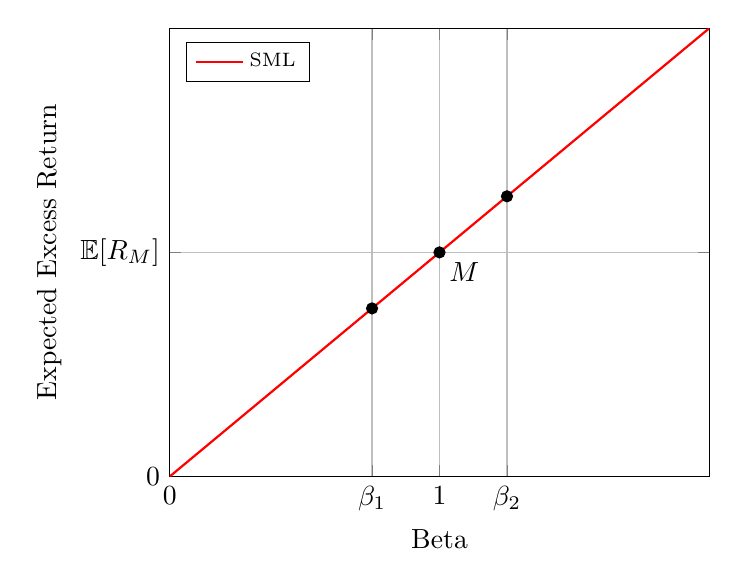
\begin{tikzpicture}
    \begin{axis}[ytick={0,1},yticklabels={0,$\mathbb{E}[R_{M}]$}, xtick={0,0.75,1,1.25}, xticklabels={0,$\beta_1$,1,$\beta_2$}, xlabel={Beta}, ylabel={Expected Excess Return}, legend pos=north west,enlargelimits=false,disabledatascaling,grid=major, legend cell align={left}]
    \addplot [domain=0:2, samples=100,red, thick]{x};
    \addlegendentry{\scriptsize SML};


    \addplot[ mark = *]coordinates {(1,1)};
    \node[below right] at (1,1) {$M$};
    \addplot[color = black, mark = *]coordinates {(0.75,0.75)};
    \addplot[color = black, mark = *]coordinates {(1.25,1.25)};

    \end{axis}
    \end{tikzpicture}
    \end{adjustbox}
    \end{frame}

\begin{frame}
    \frametitle{Tests of the CAPM}
An important question is whether the CAPM is successful in pricing assets. Empirical tests of the Sharpe-Lintner CAPM have focused on three implications:\vspace{0.25cm}\\
\begin{itemize}
    \item The intercept is zero.
    \item Beta completely captures the cross-sectional variation of expected excess returns.
    \item The market risk premium  $\mathbb{E}[z_{m,t}]$ is positive.
\end{itemize}
\end{frame}

\begin{frame}
    \frametitle{Univariate Time Series Tests}
A first strategy to test the CAPM is based on the univariate time-series regression of \cite{Black1972}:
    \begin{align}
    z_{it} = \alpha_i + \beta_iz_{m,t} + \epsilon_{i,t}, \hspace{0.5cm} \forall t \label{unitestreg}
    \end{align}
    for each asset separately, where:\vspace{0.25cm}\\
\begin{itemize}
    \item  $z$ are excess returns, i.e., $r-r_f$
    \item  the time-series behaviour of the error term, $\epsilon_{i,t}$, is assumed to be i.i.d.\vspace{0.25cm}\\
\end{itemize}
We first focus on the first implication of the model, i.e. that the intercept is zero, or to be more precise, that it is not significantly different from zero.
\end{frame}

\begin{frame}
    \frametitle{Univariate Time Series Tests}
    A first test of the CAPM may be based on the null hypothesis $H_0: \alpha_i = 0$ for all assets
    using a standard t-statistic:
    \begin{align}
        t[\hat{\alpha}_i] = \frac{\hat{\alpha}_i}{\sqrt{\hat{\mathbb{V}}[\hat{\alpha}_i]}} \hspace{1cm} 
      \end{align}
      with:      
        \begin{align}    
         \mathbb{V}[\hat{\alpha}_i] = \frac{1}{T}\left(1+\frac{\mathbb{E}[z_m]^2}{\sigma_{z_m}^2} \right)\hat{\sigma}_{\epsilon_i}^2 = \frac{1}{T}\left( 1+SR_m^2\right)\hat{\sigma}_{\epsilon_i}^2
    \end{align}
Under the null hypothesis, $t[\hat{\alpha}_i]$ is distributed as a $t(T-2)$. An equivalent test is the chi-square test based on:
\begin{align}
\frac{\alpha_i^2}{\mathbb{V}[\hat{\alpha}_i]} = \frac{\alpha_i^2}{(1+SR_m^2)\sigma_{\epsilon_i}^2/T} \label{chitest1}
\end{align}
which is distributed as a $\chi^2(1)$.
\end{frame}

\begin{frame}
    \frametitle{Multivariate Time Series Tests}
The CAPM is actually {\color{ubRed} more restrictive: all the $\alpha_i$ should be jointly equal to zero}. The null hypothesis is therefore $H_0: \alpha_1 = \hdots = \alpha_N = 0$, while the alternative hypothesis is $H_a:\exists i$ so that $\alpha_i \neq 0$. Testing $H_0$ involves the joint distribution of $\boldgreek{\alpha} = (\alpha_1,\hdots,\alpha_N)'$.\vspace{0.5cm}\\

The test of $H_0:\boldgreek{\alpha} = 0$ is the multivariate form of equation \eqref{chitest1}:
\begin{align}
    \hat{\boldgreek{\alpha}}'(\mathbb{V}[\hat{\boldgreek{\alpha}}])^{-1}\hat{\boldgreek{\alpha}} \sim \chi^2(N),
\end{align}
where $N$ is the number of assets and $\mathbb{V}[\hat{\boldgreek{\alpha}}]$ is the $N\times N$ covariance matrix of $\hat{\boldgreek{\alpha}}$. This maps to a basic Wald test.
\vfill
\begin{exampleblock}{{\small{Command}}}
In  \texttt{STATA} the relevant command for \emph{basic} Wald tests is \href{https://www.stata.com/manuals13/rtest.pdf}{\color{Purple}test}, in  \texttt{MATLAB} it is \href{https://ch.mathworks.com/help/econ/waldtest.html\#bt6pw5o-EstCov}{\color{Purple}waldtest}, and in \texttt{Python} it is statsmodels.regression.linear\_model.RegressionResults.\href{https://www.statsmodels.org/stable/generated/statsmodels.regression.linear_model.RegressionResults.wald_test.html}{\color{Purple}wald\_test}
\end{exampleblock}
\end{frame}

\begin{frame}
    \frametitle{Multivariate Time Series Tests}
    It turns out that, since the regressor $z_{m,t}$ is the same in all regressions, the covariance
    between $\hat{\alpha_i}$ and $\hat{\alpha_j}$ is:
    \begin{align}
        \mathbb{COV}[\hat{\alpha_i},\hat{\alpha_j}] = \frac{1}{T}\left(1+\frac{\mathbb{E}[z_m]^2}{\sigma_{z_m}^2} \right) \mathbb{COV}[\epsilon_{i,t},\epsilon_{j,t}]
    \end{align}
    such that the covariance matrix of $\hat{\boldgreek{\alpha}}$ maps to:
    \begin{align}
        \mathbb{V}[\hat{\boldgreek{\alpha}}] =  \frac{1}{T}\left(1+\frac{\mathbb{E}[z_m]^2}{\sigma_{z_m}^2} \right) \boldgreek{\Sigma}
    \end{align}
    where $\boldgreek{\Sigma} = \mathbb{E}[\epsilon_t\epsilon']$, i.e., the covariance matrix of the residuals from the regression in equation \eqref{unitestreg}.
\end{frame}

\begin{frame}[label=Wald]
    \frametitle{Multivariate Time Series Tests}
    In general,$\mathbb{V}[\hat{\alpha}]$  is not known and hence, this expression cannot be used directly. We have
    to preliminary estimate the covariance matrix $ \hat{\boldgreek{\Sigma}} = \frac{1}{T}\sum_{t=1}^T \hat{\epsilon}_t'\hat{\epsilon}_t$
    and then compute:
    \begin{align}
    \mathbb{\hat{V}}[\hat{\boldgreek{\alpha}}] =  \frac{1}{T}\left(1+\frac{\mathbb{E}[z_m]^2}{\sigma_{z_m}^2} \right) \hat{\boldgreek{\Sigma}}
    \end{align}
    Because $\hat{\boldgreek{\Sigma}}$ has been preliminarily estimated, the $\chi^2$ distribution only holds asymptotically under the null hypothesis. We then have the following {\color{ubRed}Wald test} statistic:
    \begin{align}
        J_0 = T\left(1+\frac{\mathbb{E}[z_m]^2}{\sigma_{z_m}^2} \right)^{-1} \hat{\boldgreek{\alpha}}' \hat{\boldgreek{\Sigma}}^{-1}\hat{\boldgreek{\alpha}} =T(1+SR_m^2)^{-1}  \hat{\boldgreek{\alpha}}' \hat{\boldgreek{\Sigma}}^{-1}\hat{\boldgreek{\alpha}} \overset{a}{\sim} \chi^2(N)
    \end{align}
The {\color{ubRed}Wald test} is based only on the estimators from an {\color{ubRed}unconstrained model}, i.e. the
intercepts are not restricted to zero. We may also consider a {\color{ubRed}Likelihood Ratio test}, which is based on the
estimators of the constrained model, i.e. the intercepts are forced to be zero. The LR test would then test for a significant difference in the covariance matrix of the residuals of the restricted and unrestricted models.\vspace{0.25cm}\\

\textbf{Note:} A multivariate version of the Wald test for multiple factors will be discussed later: \vspace{0.25cm}\\
\hyperlink{MVWald}{\beamergotobutton{Multivariate Wald Test}}


\end{frame}

\begin{frame}
    \frametitle{The GRS Test}
    The normal version of the Wald test does not recognize sampling variation in $\hat{\boldgreek{\Sigma}}$. The Gibbons, Ross, and Shanken (1989) or {\color{ubRed}GRS} test statistic can account for that and takes the form:

    \begin{align}
        J_{GRS} = {\color{ubRed}\frac{T-N-1}{N}}(1+SR_m^2)^{-1}  \hat{\boldgreek{\alpha}}' \hat{\boldgreek{\Sigma}}^{-1}\hat{\boldgreek{\alpha}} \overset{a}{\sim} {\color{ubRed}F(N,T-N-1)}
    \end{align}
    as opposed to:
    \begin{align}
        J_0 = T(1+SR_m^2)^{-1}  \hat{\boldgreek{\alpha}}' \hat{\boldgreek{\Sigma}}^{-1}\hat{\boldgreek{\alpha}} \overset{a}{\sim} \chi^2(N)
    \end{align}
    The {\color{ubRed} GRS} test is generally preferable.


\end{frame}

\begin{frame}
    \frametitle{The GRS Test}
    \begin{center}
        \includegraphics[scale=0.5]{GRS}
    \end{center}


\end{frame}

\begin{frame}
    \frametitle{Cross-Sectional Tests}
    A second approach for testing the Sharpe-Lintner version of the CAPM is based on a {\color{ubRed}two-stage procedure}\vspace{0.5cm}\\

    {\color{ubRed} The first-pass time series regression} consists of estimating the $\beta_i$ for each asset using {\color{ubRed}the time-series dimension}. Under the assumption that $\beta_i$ is constant over time, the first-pass regression is, for each asset separately:
    \begin{align}
        z_{i,t} = \alpha_i + \beta_i z_{m,t} + \epsilon_{i,t}
    \end{align}
    and yields $ \hat{\beta}_i$ as the estimate for $\beta_i$. We also expect $\alpha_i = 0$ for each asset $i$.
\end{frame}

\begin{frame}
    \frametitle{Cross-Sectional Tests}
{\color{ubRed}The second-pass cross-sectional regression} consists of regressing excess returns on betas. For each asset $i$, we compute the sample average excess return $\bar{z}_i = \bar{r}_i - \bar{r}_f$. Then, we estimate the following {\color{ubRed} cross-sectional regression}:
\begin{align}
    \bar{z}_i = \psi_0 + \psi_1\hat{\beta_i}+ v_i, \forall i
\end{align}
where $\hat{\beta_i}$ is the estimate obtained from the first-pass regression. If the CAPM is valid, then $\psi_0 = 0$, i.e. the intercept is zero, and $\psi_1 = \bar{z}_i = \bar{r}_i - \bar{r}_f$, the sample average market portfolio excess return. For instance, the test of the null hypothesis $H_0:\psi_0 = 0$ can be based on the t-statistic:
\begin{align}
    t(\hat{\psi}_0) = \frac{\hat{\psi}_0}{\hat{se}_{\hat{\psi}_0}}
\end{align}
This expression does not take into account that the regressor $\hat{\beta_i}$ has been preliminarily estimated. This introduces a {\color{ubRed} bias in the estimation of the variance} of $\hat{\psi_0}$ and $\hat{\psi_1}$.
\end{frame}

\begin{frame}
    \frametitle{Cross-Sectional Tests}
\begin{center}
    Cross-sectional results in \cite{Black1972}:\vspace{0.5cm}\\
    \includegraphics[scale=0.5]{BJS1}
\end{center}
\end{frame}

\begin{frame}
    \frametitle{Error-in-Variables in Beta}

Another econometric problem is that, in the first-pass time-series regression, the estimate $\hat{\beta_i}$ may be unbiased but it is measured with error. Hence, in the second-pass regression, there is a classic {\color{ubRed} error in variables problem}, which means that the OLS estimate of $\psi_1$ is downward biased and the estimate of $\psi_0$ is upward biased.  \vspace{0.5cm}\\
\begin{itemize}
    \item The betas used in the cross-section regression are $\hat{\beta_i} = \beta_i + u_i$
    \item The relation estimated is of the form $\bar{z}_i = \psi_0 + \psi_1\hat{\beta_i}+ v_i$
    \item While the true relation is $\bar{z}_i = \psi_0^{*} + \psi_1^{*}\beta_i+ v_i^{*}$
    \item The bias amounts to:
    \begin{align*}
        \psi_1 &=  \frac{\psi_1^{*}}{1 + \frac{\mathbb{VAR}[u_i]}{\mathbb{VAR}[\beta_i]}} \leq \psi_1^{*} \hspace{7cm}\vspace{0.5cm}\\
    \end{align*}
\end{itemize}
\cite{FAMA1973} have proposed to {\color{ubRed}group stocks into portfolios} to minimize the error in measurement in betas. In this regard, the best portfolios are those formed on the basis of past betas.
\end{frame}

\begin{frame}[label=FMB]
    \frametitle{Fama-MacBeth Procedure}

    The basic idea of \cite{FAMA1973} is, for each cross section, to project the returns on the betas and then aggregate the estimates in the time-series dimension. The estimation is performed in three steps: \vspace{0.5cm}\\
    \textbf{1.} {\color{ubRed} The first step consists of estimating betas with time-series regressions for each stock} using rolling regressions for $S$ subsamples, e.g., yearly:\vspace{0.25cm}\\
    \begin{itemize}
        \item $r_{i,t} = \alpha_i + \beta_i r_{m,t} + \epsilon_{i,t}$ within each of the $S$ subsamples for every stock $i$, where $r_i$ and $r_m$ are excess returns.
        \item $N$ portfolios are formed on the basis of ranked $\hat{\beta_i}$ of individual stocks in every subsample $S$, e.g. deciles.
        \item For each portfolio $p$ you get $S$ betas in total (here one beta for every sample year, $S$, for each portfolio $p$). The portfolio beta is a weighted beta of its constituents. \vspace{0.25cm}\\
    \end{itemize}
\textbf{2.} {\color{ubRed} Then, we run a cross-sectional regression for each subset $S$} (on portfolio level):\vspace{0.25cm}\\
\begin{itemize}
    \item $\bar{r}_{p,s} = \psi_{0,s} + \psi_{1,s}\hat{\beta}_{p,s} + u_{p,s}$, $\forall S$
    \item where $\hat{\beta}_{p,s} = K^{-1} \sum_{i=1}^{K} \hat{\beta}_{i,s}$ denotes the equally weighted portfolio beta of portfolio $p$  (of $K$ stocks) and $\bar{r}_{p,s}$ is the average portfolio excess return in susbample (year) $S$ of portfolio $p$.
\end{itemize}


\end{frame}

\begin{frame}
    \frametitle{Fama-MacBeth Procedure}

    \textbf{3.} {\color{ubRed} Then we estimate $\hat{\psi}_0$ and $\hat{\psi}_1$ as the average of the $S$ cross-sectional regressions} in step 2:\vspace{0.25cm}\\
    \begin{itemize}
        \item $\hat{\psi}_0 = S^{-1} \sum_{s=1}^S \hat{\psi}_{0,S}$ and $\hat{\psi}_1 = S^{-1} \sum_{s=1}^S \hat{\psi}_{1,s}$\vspace{0.25cm}\\
    \end{itemize}
It turns out that the standard error of the cross-sectional average is simply the standard deviation of the cross-sectional estimates divided by the square root of $S$: \vspace{0.25cm}\\
\begin{itemize}
    \item $\hat{se}(\hat{\psi}_0) = \frac{\hat{\sigma}(\hat{\psi}_0)}{\sqrt{S}}$ and $se(\hat{\psi}_1) = \frac{\hat{\sigma}(\hat{\psi}_1)}{\sqrt{S}}$ \vspace{0.25cm}\\
\end{itemize}
The test of the null hypothesis $H_0: \psi_i = x$ is based on the t-statistic:
\begin{align}
    t(\hat{\psi}_i) = \frac{\hat{\psi}_i - x}{\hat{se}(\hat{\psi}_i)} \overset{a}{\sim} t_{(S-1)}
\end{align}
One problem often found in time series data is that the error terms might be correlated over time. To that end, one is better off using {\color{ubRed}Newey–West standard errors} (\cite{Newey1987a}) for time series coefficients estimated by OLS regression, similar to robust standard errors to account for heteroskedasticity in panel data.
\end{frame}

\begin{frame}
    \frametitle{Fama-MacBeth Procedure}

An even stronger implication of the CAPM is that only $\beta_p$ should explain $r_{p,t}$. To that end, \cite{FAMA1973} also consider the following second-pass cross-sectional regression:
\begin{align}
 r_{p,t} = \psi_{0,t} + \psi_{1,t}\hat{\beta}_{p,t} + \psi_{2,t}\hat{\beta}_{p,t}^2 + \psi_{3,t}\hat{s}_{p,t}(\hat{\epsilon}_i)+ u_{p,t},
\end{align}
where $\hat{s}_{p,t}(\hat{\epsilon}_i)$ denotes the portfolio's idiosyncratic risk in period $t$. This gives raise to the following testable implications:\vspace{0.25cm}\\
\begin{itemize}
    \item If $\psi_2 \neq 0$, then there are non-linearities in the CAPM relation.
    \item If $\psi_3 \neq 0$, then non-systematic risk affects the expected portfolio return.\vspace{0.5cm}\\
\end{itemize}


\textbf{Note:} Myriad papers use Fama-MacBeth regressions. What they actually mean is that they adopt the second stage. i.e., period-by-period cross-sectional regressions and then average coefficients. This is also often used to evaluate the performance of portfolios: \hyperlink{pfAnalysis}{\beamergotobutton{Potfolio analysis}}
\vfill
\begin{exampleblock}{{\small{Command}}}
In  \texttt{STATA} the second stage of the Fama-MacBeth procedure is facilitated via ssc install \href{http://fmwww.bc.edu/repec/bocode/x/xtfmb.html}{\color{Purple}xtfmb}, including an option to implement Newey-West corrected standard errors, and in \texttt{Python} the second stage procedure is estimated using linearmodels.panel.model.\href{https://bashtage.github.io/linearmodels/panel/panel/linearmodels.panel.model.FamaMacBeth.html\#linearmodels.panel.model.FamaMacBeth}{\color{Purple}FamaMacBeth}
\end{exampleblock}
\end{frame}

%\begin{frame}
%    \frametitle{Fama-MacBeth Procedure}
%\begin{center}
%    Cross-sectional results in \cite{FAMA1973}:\vspace{0.5cm}\\
%    \includegraphics[scale=0.325]{FMB1}
%\end{center}
%\end{frame}
%
%\begin{frame}
%    \frametitle{Fama-MacBeth Procedure}
%\begin{center}
%    Cross-sectional results in \cite{FAMA1973}:\vspace{0.5cm}\\
%    \includegraphics[scale=0.325]{FMB2}
%\end{center}
%\end{frame}

\begin{frame}
    \frametitle{Empirical Issues of the CAPM}

The CAPM is an empirical failure (\cite{Black1972} and the literature that follows):\vspace{0.25cm}\\
        \begin{itemize}
        \item The econometrician does not observe the market portfolio (\cite{Roll1977}), the so-called ``Roll Critique''
        \item Suppose we could measure $\beta_n$ on each individual asset $n$ without error (this is actually a major practical issue). Then we could regress betas cross-sectionally onto unconditional expected excess returns:\begin{align}
        \begin{array}{c c}\bar{z}_i = \psi_0 + \psi_1\hat{\beta_i}+ v_i, \forall i, & n=1,...,N\end{array}
        \end{align}
        \item The CAPM directly implies that the intercept of this regression is zero, $\psi_0\equiv 0$, and the slope is the market risk premium, $\psi_1=\mathbb{E}[r_{m,t} -  r_{f,t}]$.
        \item When running this regression empirically, we typically find that $\psi_0$ is statistically different from zero and the CAPM is way too flat (its slope is much less than $\approx 6\%$).
        \item Beta simply cannot explain variations in expected returns.
    \end{itemize}
\end{frame}

\begin{frame}
\frametitle{Empirical Issues of the CAPM}
\centering
\begin{adjustbox}{width=\textwidth,height=0.7\textheight,keepaspectratio}
\begin{tikzpicture}
\only<1-2>{\begin{axis}[ytick={0,1},yticklabels={0,$\mathbb{E}[R_{M}]$}, xtick={0,0.25,0.75,1,1.25,1.75}, xticklabels={0,$\widehat{\beta}_1$,$\beta_1$,1,$\beta_2$,$\widehat{\beta}_2$}, xlabel={Beta}, ylabel={Expected Excess Return}, legend pos=north west,enlargelimits=false,disabledatascaling,grid=major, legend cell align={left}]
\addplot [domain=0:2, samples=100,dashed, thick]{x};
    \addlegendentry{\scriptsize Theoretical SML};

\addplot[ mark = *]coordinates {(1,1)};
\node[below right] at (1,1) {$M$};
\addplot[color = black, mark = *]coordinates {(0.75,0.75)};
\addplot[color = black, mark = *]coordinates {(1.25,1.25)};

\only<2->{\addplot[color = red, mark = *]coordinates {(0.25,0.75)};
\addplot[color = red, mark = *]coordinates {(1.75,1.25)};}
\only<2->{\draw[latex-] (0.28,0.75) -- (0.75,0.75);
\draw[-latex] (1.25,1.25) -- (1.72,1.25);}

\end{axis}}

\only<3>{\begin{axis}[ytick={0,0.67,1},yticklabels={0,$\alpha$,$\mathbb{E}[R_{M}]$}, xtick={0,0.25,0.75,1,1.25,1.75}, xticklabels={0,$\widehat{\beta}_1$,$\beta_1$,1,$\beta_2$,$\widehat{\beta}_2$}, xlabel={Beta}, ylabel={Expected Excess Return}, legend pos=north west,enlargelimits=false,disabledatascaling,grid=major, legend cell align={left}]
\addplot [domain=0:2, samples=100,dashed, thick]{x};
    \addlegendentry{\scriptsize Theoretical SML};
\addplot [domain=0:2, samples=100,red, thick]{0.666+0.333*x};
    \addlegendentry{\scriptsize Observed SML};
\addplot[color=blue, thick] coordinates {(0,0) (0,0.67)};
    \addlegendentry{\scriptsize Intercept};
\addplot[color = blue, mark = *]coordinates {(0,0.67)};

\addplot[ mark = *]coordinates {(1,1)};
\node[below right] at (1,1) {$M$};
\addplot[color = black, mark = *]coordinates {(0.75,0.75)};
\addplot[color = black, mark = *]coordinates {(1.25,1.25)};

\addplot[color = red, mark = *]coordinates {(0.25,0.75)};
\addplot[color = red, mark = *]coordinates {(1.75,1.25)};
\draw[latex-] (0.28,0.75) -- (0.75,0.75);
\draw[-latex] (1.25,1.25) -- (1.72,1.25);

\end{axis}}

\end{tikzpicture}
\end{adjustbox}

\end{frame}


\begin{frame}
    \frametitle{Empirical Issues of the CAPM}
    \begin{itemize}
		\item Yet the CAPM remains to this day the model most widely used by practitioners to make investment decisions and compute the cost of capital.
		\item Furthermore, the CAPM does sometimes work:\vspace{0.25cm}\\
		\begin{center}
		\begin{adjustbox}{width=0.8\textwidth,height=0.8\textheight,keepaspectratio}
		\begin{tikzpicture}
		\begin{groupplot}[group style={group size=2 by 1, horizontal sep=2.5cm}, height=0.55\textwidth, width=0.7\textwidth]
		\nextgroupplot[title={\textcolor{blue}{\cite{Savor2014a}}}, grid=major, xmin=0.4, xmax=1.8, ymin=-2, ymax=18, xlabel={Beta}, ylabel={Expected return (bps)}, legend pos=north west, legend cell align={left}]
			\addplot[thick,red] {-0.89+10.24*x};
			\addlegendentry{\scriptsize Announcement days};
			\addplot[thick,blue,densely dashed] {2.49-1.53*x};
			\addlegendentry{\scriptsize Non-announcement days};
			\addplot[only marks,red,mark size=2.5,mark=triangle*] file {SWup.dat};
			\addplot[only marks,blue,mark size=2,mark=square*] file {SWdown.dat};
			\addplot[very thick,densely dotted, black] {2+1*x};
		\nextgroupplot[title={\textcolor{blue}{\cite{Hendershott2018a}}}, grid=major, xmin=0.4, xmax=1.9, ymin=-10, ymax=22, xlabel={Beta}, ylabel={}, legend pos=north west, legend cell align={left}]
			\addplot[thick,red] {-6.7+14.1*x};
			\addlegendentry{\scriptsize Close-to-Open (Night)};
			\addplot[thick,blue,densely dashed] {18.6-15.3*x};
			\addlegendentry{\scriptsize Open-to-Close (Day)};
			\addplot[only marks,red,mark size=2.5,mark=triangle*] file {HLRup.dat};
			\addplot[only marks,blue,mark size=2,mark=square*] file {HLRdown.dat};
			\addplot[very thick,densely dotted, black] {3.5+1*x};
		\end{groupplot}
		\end{tikzpicture}
		\end{adjustbox}
		\end{center}
	\end{itemize}
%    Why do we keep rejecting it?
\end{frame}

%\begin{frame}
%    \frametitle{Empirical Issues of the CAPM}
%To derive the CAPM literature has made several assumptions:\vspace{0.25cm}\\
%\begin{enumerate}
%		\item Investors have homogeneous beliefs regarding end-of-period returns.
%		\item Returns follow an elliptic distribution.
%		\item Investors choose portfolios to maximize their end-of-period expected utility of wealth, and exhibit concave and increasing utility.
%		\item Investors can take long or short position of any size in any asset, and may borrow or lend any amount at the riskless rate.\vspace{0.25cm}\\
%		\end{enumerate}
%	Lintner (JFQA, 1969) has shown that removing assumption (1) does not change the structure of capital asset prices in any significant way, and assumptions (2) and (3) are usually regarded as acceptable approximations to reality. Assumption (4), however, is not a very good approximation for many investors, and one feels that the model would be changed substantially if this assumption were dropped (Black, 1972).
%\end{frame}




\begin{frame}
    \frametitle{Multi-Factor Models}

    To summarize, the CAPM (or single-factor model) is often rejected by the data, because of its overly
    simplistic implications, first and foremost:\vspace{0.25cm}\\
    \begin{itemize}
        \item The market beta is enough to capture all the dispersion in expected returns across assets.\vspace{0.25cm}
    \end{itemize}

    Multi-factor models try to model the various types of systematic risk on top of the market risk and how these
    risks are priced.

\end{frame}

\begin{frame}
    \frametitle{Multi-Factor Models}

The basic idea of multi-factor models is that the expected return of the investor for holding a given stock is a linear combination of the
various sources of risk of the stock times the prices of the respective risk:
\begin{align}
    \E[r_{i,t}] &= \mu_i = \lambda_0 + \lambda_1\beta_{1,i}+\hdots+\lambda_K\beta_{K,i} = \lambda_0 + \sum\limits_{k=1}^K \lambda_k\beta_{k,i} 
 \end{align}   
 or in matrix notation:
  \begin{align}  
    \E[\boldgreek{r}_t] &=\boldgreek{\mu} = \bm{1}\lambda_0 + \bm{B}\boldgreek{\lambda}
\end{align}
where $\lambda_0$ is the risk-free rate, $\lambda_k$ is the risk premium on risk factor $k$, $\bm{1} $ is a vector of ones, and $\boldgreek{\lambda}$ is the vector of the $K$ risk premia. We generally distinguish between three different types of factors:\vspace{0.25cm}\\
\begin{itemize}
    \item {\color{ubRed}Factors are observed portfolios of traded assets}
    \item {\color{ubRed}Statistical factors}
    \item Factors are observed macroeconomic variables but not traded assets
\end{itemize}
\end{frame}

\begin{frame}
    \frametitle{Factors are observed portfolios}
$N$ excess returns are linearly related to $K$ factors such that we have:
\begin{align}
    \bm{Z}_t = \boldgreek{\alpha} + \bm{B}\bm{F}_{K,t} + \boldgreek{\epsilon}_t
\end{align}
where $\bm{B}$ is a $(N\times K)$ sensitivity matrix and with: \vspace{0.25cm}\\
\begin{itemize}
    \item $\E [\boldgreek{\epsilon}_t]=0$
    \item $\E[\boldgreek{\epsilon}_t \boldgreek{\epsilon}_t']=\boldgreek{\Sigma}$
    \item $\E[\bm{F}_{K,t}]=\boldgreek{\mu}_K$
    \item $\E[(\bm{F}_{K,t} - \boldgreek{\mu}_K)' (\bm{F}_{K,t} - \boldgreek{\mu}_K)] = \boldgreek{\Omega}_K$
    \item $\mathbb{COV}[\bm{F}_{K,t}, \boldgreek{\epsilon}_t] = 0$ \vspace{0.25cm}\\
\end{itemize}

We assume that the $K$ factors capture the entire cross covariance between asset returns
so that the variance of $\boldgreek{\epsilon}_t$ is diagonal. Then the covariance matrix of returns is the sum
of two components:
\begin{align}
    \boldgreek{\Omega} = \bm{B}\boldgreek{\Omega}_K \bm{B}' + \boldgreek{\Sigma}
\end{align}
\end{frame}

\begin{frame}[label=MVWald]
    \frametitle{Factors are observed portfolios}
Similar to testing the CAPM we can test for constrained models whether the intercepts are jointly zero, i.e., $H_0= \alpha_1 =\hdots= \alpha_N$, where:
\begin{align}
    \boldgreek{\alpha} = \boldgreek{\mu} - \bm{B}\boldgreek{\mu}_K
\end{align}
The asymptotic test of $H_0: \boldgreek{\alpha} = 0$ is based on the {\color{ubRed}multivariate Wald test} statistic:
\begin{align}
    J_0 = T(1+\hat{\boldgreek{\mu}}_K' \hat{\boldgreek{\Omega}}_K^{-1} \hat{\boldgreek{\mu}}_K)^{-1} \hat{\boldgreek{\alpha}}' \hat{\boldgreek{\Sigma}}^{-1}\hat{\boldgreek{\alpha}} \overset{a}{\sim} \chi^2(N)
\end{align}
with:
\begin{align}
    \hat{\boldgreek{\Omega}}_K = T^{-1} \sum\limits_{t=1}^T (\bm{F}_{K,t} - \boldgreek{\mu}_K)' (\bm{F}_{K,t} - \boldgreek{\mu}_K)        
\end{align}
The multivariate GRS test statistic takes the form:
\begin{align}
    J_{GRS} = \frac{T-N-K}{N}(1+\hat{\boldgreek{\mu}}_K' \hat{\boldgreek{\Omega}}_K^{-1} \hat{\boldgreek{\mu}}_K)^{-1} \hat{\boldgreek{\alpha}}' \hat{\boldgreek{\Sigma}}^{-1}\hat{\boldgreek{\alpha}} \overset{a}{\sim} F(N,T-N-K)
\end{align}

The univariate Wald test can be re-examined here: \hyperlink{Wald}{\beamergotobutton{Wald test}}
\end{frame}

\begin{frame}
    \frametitle{Factors are observed portfolios}
\textbf{Examples:} \cite{Fama1992} propose the seminal {\color{ubRed} three-factor model}:\vspace{0.25cm}\\
\begin{itemize}
    \item Expected return of the market portfolio –  {\color{ubRed}market risk premium (MRP)}
    \item Difference between the return on a portfolio of firms with a low market value of
equity (small cap) and the return on a portfolio of firms with a high market
value of equity (large cap) – {\color{ubRed}small minus big (SMB) factor}
\item Difference between the return on a portfolio of firms with a high book-to-market
value (value stocks) and the return on a portfolio of firms with a low book-to market
value (growth stocks) – {\color{ubRed} high minus low (HML) factor}\vspace{0.25cm}\\
\end{itemize}
Another important factor is the  {\color{ubRed}momentum factor} by \cite{Carhart1997} : difference between the return on
a portfolio of firms with a low prior return (between months $t-13$ and $t-2$) (losers) and
the return on a portfolio of firms with a high prior return (between months $t-13$ and $t-2$)
(winners).
\end{frame}

\begin{frame}
    \frametitle{Statistical Factors}
    The idea of the statistical approaches is to reduce the dimension of the cross-sectional
    dimension. We have a large number of stock returns that we try to summarize with a
    small number of factors.\vspace{0.25cm}\\

    \begin{itemize}
        \item In this approach, the factors are not known, so that we need to generate the factors. There are different ways to estimate the factors among correlated financial series.
        \item Factor models are also extremely useful in the context of large portfolios.
        When we have a lot of assets in the portfolio, a complete model for all the assets
        simultaneously is not possible. In this case, we summarize the information contained in
        all the assets through a factor model (with a small number of factors) and we model the
        factors instead of the assets.
    \end{itemize}
\end{frame}

\begin{frame}
    \frametitle{Principal Component Analysis}
    One of the most widely used techniques is the principal component analysis (PCA). The main goal of PCA is to reduce the dimensionality of correlated data by identifying a small number of uncorrelated linear combinations that explain most of the variability in the original data.\vspace{0.25cm}\\
    \begin{itemize}
        \item PCA is a data-reduction technique. It determines what the drivers of a data sample are
However, it does not explain why they are the drivers of the data or what they are in the first place.
        \item PCA is based on the spectral decomposition of the covariance (or correlation) matrix.
        \item PCA is often used to summarize the information in the term structure of
interest rates.
    \end{itemize}
\end{frame}



\begin{frame}
    \frametitle{Principal Component Analysis}
\begin{center}
    \includegraphics[scale=0.35]{PCA}
\end{center}
\end{frame}


\begin{frame}
    \frametitle{Principal Component Analysis}

    \begin{block}{Spectral Decomposition Theorem}
Any symmetric matrix $\boldgreek{\Sigma} \in \mathbb{R}^{N\times N}$ can be written as
\begin{align}
    \boldgreek{\Sigma} = \boldgreek{\Gamma} \boldgreek{\Lambda} \boldgreek{\Gamma}^{-1} = \boldgreek{\Gamma} \boldgreek{\Lambda} \boldgreek{\Gamma}'
\end{align}
where \vspace{0.25cm}\\
\begin{itemize}
    \item $\boldgreek{\Lambda} = diag(\lambda_1,\hdots,\lambda_N)$ is the diagonal matrix of {\color{ubRed} eigenvalues} of $\boldgreek{\Sigma}$. The eigenvalues are ordered so that $\lambda_1 \geq \hdots \geq \lambda_N$
    \item $\boldgreek{\Gamma}$ is an orthogonal matrix satisfying $\boldgreek{\Gamma}\boldgreek{\Gamma}'=\boldgreek{\Gamma}'\boldgreek{\Gamma}=\bm{I}_N$, whose columns are the standardized {\color{ubRed} eigenvectors} of $\boldgreek{\Sigma}$ or, put differently, factor loadings.
\end{itemize}
\end{block}
{\color{ubRed}Properties} when $\boldgreek{\Sigma}$ is the covariance matrix of $\bm{r}_t$:\vspace{0.25cm}\\
\begin{itemize}
    \item The first principal component explains the greatest amount of the total variation of
$\bm{r}_t$ , the second component explains the greatest amount of the remaining variation,
and so on.
\item The principal components are orthogonal to one another.
\end{itemize}
\end{frame}

\begin{frame}
    \frametitle{Principal Component Analysis}
The dimensions of $\boldgreek{\Lambda}$ are:\vspace{0.25cm}\\
\begin{center}
    $\boldgreek{\Lambda} =
    \begin{bmatrix}
    \lambda_1 & 0 &  \hdots &0\\
    0 & \lambda_2 &  \hdots &0\\
    \vdots & \vdots & \ddots & \vdots\\
    0 & 0 & \hdots & \lambda_N
\end{bmatrix}_{N\times N}$ \vspace{0.5cm}\\
\end{center}
and the dimensions of $\boldgreek{\Gamma}$ are:\vspace{0.25cm}\\
\begin{center}
    $\boldgreek{\Gamma} = \left[\boldgreek{\Gamma}_1 \hspace{0.2cm} \boldgreek{\Gamma}_2 \hspace{0.2cm} \hdots \hspace{0.2cm} \boldgreek{\Gamma}_N \right] =
    \begin{bmatrix}
    \gamma_{1,1} & \gamma_{2,1} &  \hdots &\gamma_{N,1}\\
    \gamma_{1,2} & \gamma_{2,2} &  \hdots &\gamma_{N,2}\\
    \vdots & \vdots & \ddots & \vdots\\
    \gamma_{1,N} & \gamma_{2,N} & \hdots & \gamma_{N,N}
\end{bmatrix}_{N\times N}$
\end{center}


\end{frame}


\begin{frame}
    \frametitle{Principal Component Analysis}
    Once we have obtained the eigenvalues
    $\boldgreek{\Lambda}$ and the eigenvectors $\boldgreek{\Gamma}$, we can deduce the {\color{ubRed}principal components}:
    \begin{align}
        \boldgreek{P}_t = \boldgreek{\Gamma}'(\bm{r}_t - \boldgreek{\mu}) \text{,     with     } \boldgreek{\mu} = \E[\bm{r}_t]
    \end{align}
    In particular, the first principal component is defined as:
    \begin{align}
        \bm{P}_{1,t} = \boldgreek{\Gamma}_1'(\bm{r}_t - \boldgreek{\mu}) = \gamma_{1,1}(r_{1,t}-\mu_1)+\hdots+ \gamma_{1,N}(r_{N,t}-\mu_N)
    \end{align}
    It satisfies $\max\{\mathbb{VAR}[\boldgreek{\Gamma}_n'(\bm{r}_t - \boldgreek{\mu})]\}$, for $n=\{1,\hdots,N\}$\vspace{0.25cm}\\
    The second principal component is the standardized linear combination of $\bm{r}_t$ with
maximal variance among all linear combinations that are orthogonal to the first
principal component, and so on. We also have:\vspace{0.25cm}\\
\begin{itemize}
    \item $\E[\bm{P}_t] = 0$
    \item $\mathbb{COV} [\bm{P}_t] =\boldgreek{\Gamma}'\boldgreek{\Sigma}\boldgreek{\Gamma} = \boldgreek{\Gamma}'\boldgreek{\Gamma}\boldgreek{\Lambda}\boldgreek{\Gamma}'\boldgreek{\Gamma} = \boldgreek{\Lambda}$, i.e., the principal components are uncorrelated
\end{itemize}
\end{frame}

\begin{frame}
    \frametitle{Principal Component Analysis}
    To measure the ability of the first few principal components to explain the variability in $\bm{r}_t$, we notice that:
    \begin{align}
        \sum\limits_{i=1}^N \V[\bm{P}_{i,t}] = \sum\limits_{i=1}^N \lambda_i = trace(\boldgreek{\Sigma}) = \sum\limits_{i=1}^N \V[\bm{r}_{i,t}]
    \end{align}
    Then, for $K \leq N$, the ratio $\sum_{i=1}^K \lambda_i / \sum_{i=1}^N \lambda_i$ represents the amount of the variability
explained by the first K principal components.\vspace{0.25cm}\\
{\color{ubRed} Remark:} If the data $\bm{r}_t$ have very different sample variances (with different scales),
applying the PCA to the covariance matrix may raise some issues, because the
variables with the highest variance will dominate the first principal component. In these
situations, it is recommended to standardize the data and use the correlation matrix
instead.
\vfill
\begin{exampleblock}{{\small{Command}}}
In \texttt{STATA} the relevant command for the PCA is \href{https://www.stata.com/manuals13/mvpca.pdf}{\color{Purple}pca} or \href{https://www.stata.com/manuals13/mvpca.pdf}{\color{Purple}pcamat}, in \texttt{MATLAB} it is \href{https://ch.mathworks.com/help/stats/pca.html}{\color{Purple}pca}, and in \texttt{Python} it is  sklearn.decomposition.\href{https://scikit-learn.org/stable/modules/generated/sklearn.decomposition.PCA.html}{\color{Purple}PCA}
\end{exampleblock}
\end{frame}

\begin{frame}
    \frametitle{Principal Component Analysis}
    Finally, the principal component transform:
    \begin{align}
        \bm{P}_t = \boldgreek{\Gamma}'(\bm{r}_t - \boldgreek{\mu})
    \end{align}
can be inverted to the following equation:
\begin{align}\label{eqn:PCA_prediction}
    \bm{r}_t = \boldgreek{\mu} +  \boldgreek{\Gamma}\bm{P}_t
\end{align}
If we think the first $K$ factors are enough to explain most of the variability in $\bm{r}_t$, we
obtain the following factor representation:
\begin{align}
    \bm{r}_t = \boldgreek{\mu} + \boldgreek{\gamma}_1 \bm{P}_{1,t} +\hdots+  \boldgreek{\gamma}_K \bm{P}_{K,t} + \boldgreek{\epsilon}_t
\end{align}
where the $\boldgreek{\epsilon}_t$ capture the effect of the remaining $N-K$ principal components and are
orthogonal to the first $K$ components.
\end{frame}

\begin{frame}
    \frametitle{Principal Component Analysis}
\textbf{Example 1:} PCA of yield curve change\vspace{0.25cm}\\
    A major problem in estimating the term structure (or change thereof) is the high dimensionality of the yield curve. Using a PCA, the first three principal components map to {\color{Cerulean}level}, {\color{RedOrange}slope}, and {\color{Peach}curvature} of yield curves (Swiss data):
\begin{center}

    \includegraphics[scale=0.15]{tsPCA}
\end{center}
\end{frame}

\begin{frame}
    \frametitle{Principal Component Analysis}
\textbf{Example 1:} PCA of yield curve change\vspace{0.25cm}\\
First three yield curve loadings:
\begin{itemize}
    \item First loading is roughly flat: parallel shifts of the yield curve ({\color{ubRed}level})
    \item Second loading is upward sloping: tilting of the yield curve ({\color{ubRed}slope})
    \item Third loading is hump-shaped: flexing of the yield curve ({\color{ubRed}curvature})
\end{itemize}
\end{frame}


\begin{frame}
    \frametitle{Principal Component Analysis}
\textbf{Example 2:} Jondeau, Jurczenko, and Rockinger (2016) conduct a PCA for 44 international stock markets between July 1994 and December 2014 (1068 weekly observations). The data are log-returns in US dollar.\vspace{0.25cm}\\
\begin{center}
    \includegraphics[scale=0.4]{PCA1}
\end{center}
\end{frame}

\begin{frame}
    \frametitle{Principal Component Analysis}

\begin{center}
    \includegraphics[scale=0.4]{PCA2}
\end{center}
\end{frame}

\begin{frame}
    \frametitle{Principal Component Analysis}
\textbf{Example 3:} \cite{Baker2006} study how investor sentiment affects the cross-section of stock returns. To that end, they conduct a PCA to construct a market sentiment index to capture investors' attitude regarding the stock market. They choose a set of variables of which each is supposed to proxy for market sentiment, such as the number of IPOs, first-day returns, etc. In order to filter out and aggregate common factors underlying different sentiment variables they conduct a PCA and construct a sentiment index using the first principal component.\\

\end{frame}


\begin{frame}
    \frametitle{Reading Tip}
Campbell, John Y., A. W. Lo, and A. C. MacKinlay (1997), The Econometrics of Financial Markets, Princeton\vspace{0.35cm}\\
\begin{center}

    \includegraphics[scale=0.35]{Campbell}
\end{center}
\end{frame}

\begin{frame}[label={end_curriculum}]
    \frametitle{Practice Session - Beat the clock}
    If any one successfully completes the tasks before class is over, all students will receive 5 bonus points in the second assignment. You can work together, alone (diversification!), or split into groups (optimization!). The best solution is relevant.\vspace{1cm}\\
    
Using the Swiss government bonds data on ILIAS, complete the following tasks:
\begin{enumerate}[1)]
	\item Run a PCA on the time series of Swiss government bonds. For the entire exercise, keep in mind that Stata automatically standardizes variables in the PCA, i.e $z = \frac{r-\mu}{\sigma}$. How much variation do the first three principal components explain?
	\item Plot the the factor loadings for the first three principal components (Hint: ssc install eofplot). Are the loadings (more or less) equivalent to the ones on slide 109?
	\item Generate the time series for the first principal component (Hint: predict)
	\item Compute the fitted time series for the 10 Year government bond using the first principal component and plot it together with the actual time series (Hint: Use equation \eqref{eqn:PCA_prediction} but keep in mind that factor loadings pertain to standardized variables, $z$.)
\end{enumerate}


\vfill

As time passes, I will display code snippets that should help you deal with certain aspects of the tasks!

\end{frame}


\begin{frame}
    \begin{center}
        {\color{ubRed} \Huge{Additional Topics}}
    \end{center}
\end{frame}


\begin{frame}[label=TS]
    \begin{center}
        {\color{ubRed} \Huge{Time Series Models}}
    \end{center}
\end{frame}

\begin{frame}
    \frametitle{Time Series Models}
    The objectives of this chapter are the following:\vspace{0.25cm}\\
    \begin{itemize}
        \item General idea of predictive time series models
        \item Understanding the autoregressive model (AR)
        \item Understanding the moving average model (MA)
        \item Understanding the autoregressive moving average model (ARMA/ARIMA)
        \item Maximum Likelihood Estimation
    \end{itemize}
\end{frame}

\begin{frame}
    \frametitle{General Idea of Time Series Models}
So far, we have mostly dealt with the question of how to test whether asset returns fulfil the assumptions imposed by literature, how to test whether fundamental asset pricing models hold, and how to test whether markets are efficient. We will now shift the scope of the course towards the predictability of financial time series using time series models. \vspace{0.25cm}\\

The general idea of time series models is that {\color{ubRed}time series are governed by some underlying dynamics}. To that end, {\color{ubRed}time series models aim at capturing and representing these dynamics} in order to make predictions about its future path. Most models require that the time series be:\vspace{0.25cm}\\
\begin{itemize}
    \item weakly (covariance) stationary
    \item ergodic
\end{itemize}
\end{frame}

\begin{frame}
    \frametitle{Autoregressive Model}

A straight forward model is the autoregressive model (AR). It describes the dynamics of a time series as a function of its past realizations. For instance, if we expect that the current realization is a function of the prior realization only, i.e., one lag, we have the following first-order AR(1) process:
\begin{align}
    X_t = c + \phi X_{t-1} + \epsilon_t
\end{align}
where $c$ is a constant (intercept) and $\epsilon_t$ is white noise, i.e., an error term with zero mean and finite variance, often referred to as shock or innovation. More generally, we can write the p$^{th}$ order AR($p$) process as follows:
\begin{align}
    X_t = \mu + \sum\limits_{i=1}^p\phi_i X_{t-i} + \epsilon_t
\end{align}
What we essentially have, is a regression of a variable on $p$ lags of itself. Instead of OLS, one can also use maximum likelihood estimation.

\end{frame}

\begin{frame}
    \frametitle{Moving Average Model}

    Another essential representation of time series dynamics is the moving average model (MA). It represents the time series as a linear combination of contemporaneous and past realizations of shocks $\epsilon$, i.e., error terms. For instance, if we expect that the current realization is a function of the current and prior realization of the shock only, i.e., one lag, we have the following first-order MA(1) process:
\begin{align}
    X_t = c + \epsilon_t +\theta \epsilon_{t-1}
\end{align}
 The name moving average comes from the fact that $X_t$ is a weighted average of contemporaneous and past shocks. More generally  we can write the q$^{th}$ order MA(1) process as follows:
 \begin{align}
     X_t = \mu +\epsilon_{t}+ \sum\limits_{i=1}^q\theta_i \epsilon_{t-i}
 \end{align}
 Note that fitting the MA estimates is more complicated than it is in AR models, because the {\color{red}lagged error terms are not observable}. This means that iterative non-linear fitting procedures need to be used in place of linear least squares.
\end{frame}

\begin{frame}
    \frametitle{AR($p$) Model vs. MA($q$) Model}
    Some important differences between the AR and MA models are:\vspace{0.25cm}\\
    \begin{itemize}
        \item The primary difference between an AR and MA model is based on the correlation between time series observations at different points in time. The covariance between $X_t$ and $X_{t-1}$ is zero for MA models. However, the correlation of $X_t$ and $X_{t-1}$ gradually declines with $p$ becoming larger in AR models.
        \item The AR($p$) model uses the past forecasts to predict future values.
        \item The moving average model specifies that the output variable depends linearly on the current and various past values of a stochastic (imperfectly predictable) term. Rather than using the past values of the forecast variable in a regression, a moving average model uses past forecast errors in a regression-like model.
    \end{itemize}

\end{frame}

\begin{frame}
    \frametitle{Autoregressive Moving Average Model}
The autoregressive moving average model (ARMA) describes weakly stationary stochastic time series in terms of two polynomials:\vspace{0.25cm}\\
\begin{itemize}
    \item An autoregressive polynomial of order $p$ to capture autocorrelation.
    \item An moving average polynomial of order $q$ to account for the persistence in shocks.\vspace{0.25cm}\\
\end{itemize}
In essence, it is a model with $p$ autoregressive terms and $q$ moving average terms such that it maps to nothing different than a combination of an AR($p$) model and a MA($q$) model. In general, a  ARMA($p$,$q$) model has the following form:
\begin{align}
    X_t = c + \epsilon_t +  \sum\limits_{i=1}^p\phi X_{t-i} +  \sum\limits_{i=1}^q\theta \epsilon_{t-i}
\end{align}
An extension of the ARMA($p$,$q$) model is the ARIMA($p$,$d$,$q$) model where $d$ specifies the order of integration $I$ of a time series.
\vfill
\begin{exampleblock}{{\small{Command}}}
In  \texttt{STATA} the relevant command for the AR(I)MA family is \href{https://www.stata.com/manuals13/tsarima.pdf}{\color{Purple}arima}, in \texttt{MATLAB} it is also \href{https://ch.mathworks.com/help/econ/arima.html;jsessionid=8072254506805dd340ee28abd6fb}{\color{Purple}arima}, and in \texttt{Python} it is statsmodels.tsa.arima\_model.\href{https://www.statsmodels.org/stable/generated/statsmodels.tsa.arima_model.ARIMA.html}{\color{Purple}ARIMA}
\end{exampleblock}
\end{frame}



\begin{frame}
    \frametitle{Estimating Time Series Models}
Technically, one can resort to any fitting methodology that minimizes some error term. However, convention suggests one of the following two:\vspace{0.25cm}\\
\begin{itemize}
    \item {\color{ubRed}Maximum likelihood}
    \item Least squares family, if feasible\vspace{0.25cm}\\
\end{itemize}

The procedure to estimate the model parameters looks as follows:\vspace{0.25cm}\\
\begin{enumerate}[1.]
    \item Choose some (arbitrary) initial model parameters and predict the model outcome for each period in your data sample.
    \item Compare the predicted values (fit) with the actual outcome in all periods $t$ and assess the most effective parameter changes to improve your fit.
    \item Change the model parameters and repeat step 2 until the fit can no longer be improved, i.e., the model converged to the optimum.
\end{enumerate}
\end{frame}

\begin{frame}
    \frametitle{Maximum Likelihood Estimation}
    The MLE principle provides a means of estimating a parameter or set of parameters, $\boldgreek{\Theta}$, by maximizing a likelihood function, so that under the assumed statistical model the observed data is most \emph{likely}.\vspace{0.25cm}\\
    \begin{block}{Maximum Likelihood Estimation}
        Given some PDF of error terms and observations $X_t \in \{X_1,\hdots,X_T\}$
    \begin{align}
        L_T(\boldgreek{\Theta}) = \prod\limits_{t=1}^T f(X_t;\boldgreek{\Theta})
    \end{align}
is known as the {\color{ubRed}likelihood function}. The likelihood equation for the {\color{ubRed}maximum} is
\begin{align}
    \nabla \ln(L_T(\boldgreek{\Theta})) = \frac{\partial \ln(L_T(\boldgreek{\Theta}))}{\partial \boldgreek{\Theta}} = 0
\end{align}
\end{block}
\end{frame}

\begin{frame}
    \frametitle{Maximum Likelihood Estimation}
\begin{center}
    \begin{tikzpicture}[ % Define Normal Probability Function
declare function={
            normal(\x,\m,\s) = 1/(2*\s*sqrt(pi))*exp(-(\x-\m)^2/(2*\s^2));
        }
       ]
\begin{axis}[
    no markers,
    domain=0:12,
    zmin=0, zmax=1,
    xmin=0, xmax=3,
    samples=200,
   samples y=0,
    axis lines=middle,
    xtick={0.5,1.5,2.5},
    xmajorgrids,
    xticklabels={},
    ytick=\empty,
    xticklabels={$x_1$, $x_2$, $x_3$},
    ztick=\empty,
    xlabel=$x$, xlabel style={at={(rel axis cs:1,0,0)}, anchor=west},
    ylabel=$y$, ylabel style={at={(rel axis cs:0,1,0)}, anchor=south west},
    zlabel=Likelihood, zlabel style={at={(rel axis cs:0,0,0.5)}, rotate=90, anchor=south},
    set layers,
    scale=1.5
  ]

\addplot3 [samples=2, samples y=0, domain=0:3] (x, {1.5*(x-0.5)+3}, 0);
\only<1>{\addplot3 [cyan!0!black!0, thin, dotted] (2.5, x, {normal(x, 3, 1)});}


%\only<2->{\addplot3 [cyan!0!black!0, thick] (0.5, x, {normal(x, 3, 1)});}
\only<2->{\addplot3 [cyan!50!black, thick] (0.5, x, {normal(x, 3, 1)});}
\only<2->{\addplot3 [cyan!50!black, thick] (1.5, x, {normal(x, 4.5, 1)});}
\only<2->{\addplot3 [cyan!50!black, thick] (2.5, x, {normal(x, 6, 1)});}

\pgfplotsextra{
\begin{pgfonlayer}{axis background}
    \node at (0.5, 3.5, 0)[circle,fill,inner sep=1pt]{};
    \node at (1.5, 3.5, 0)[circle,fill,inner sep=1pt]{};
    \node at (2.5, 6.5, 0)[circle,fill,inner sep=1pt]{};

\only<3->{\draw [on layer=axis background,red,thick] (0.5, 3.5, 0) -- (0.5, 3.5, {normal(0,0,1.15)});}
\only<2->{\draw [thick, dotted] (0.5, 3, 0) -- (0.5, 3, {normal(0,0,1)});}
\only<2->{\draw (0.5,0,0) -- (0.5,12,0);}

\only<3->{\draw [red,thick] (1.5, 3.5, 0) -- (1.5, 3.5, {normal(0,0,1.65)});}
\only<2->{\draw [thick, dotted] (1.5, 4.5, 0) -- (1.5, 4.5, {normal(0,0,1)});}
\only<2->{\draw (1.5,0,0) -- (1.5,12,0);}

\only<3->{\draw [red,thick] (2.5, 6.5, 0) -- (2.5, 6.5, {normal(0,0,1.15)});}
\only<2->{\draw [thick, dotted] (2.5, 6, 0) -- (2.5, 6, {normal(0,0,1)});}
\only<2->{\draw (2.5,0,0) -- (2.5,12,0);}


\end{pgfonlayer}
}
\end{axis}
\end{tikzpicture}
\end{center}
\end{frame}


\begin{frame}
    \frametitle{Maximum Likelihood Estimation}
    The ML estimator is obtained by maximizing the likelihood. Since logarithmic functions are injective on the domain $(0,\infty]$, this is equivalent to
maximizing the {\color{ubRed}log-likelihood function}:
\begin{align}
    \argmax_{\boldgreek{\Theta}} \hspace{0.25cm} \ln(L_T(\boldgreek{\Theta})) = \ell_T(\boldgreek{\Theta}) = \sum\limits_{t=1}^T  \ell_t(\boldgreek{\Theta})
\end{align}
where:
\begin{align}
    \ell_t(\boldgreek{\Theta}) = -\frac{1}{2}\left( \ln(2\pi)+\ln(\sigma_t^2)+\frac{\epsilon_t^2}{\sigma_t^2} \right)\label{eq:loglikelihood}
\end{align}
is the log-likelihood of the observation in period $t$, assuming {\color{ubRed} a normal distribution} for the error terms. The first-order derivative vector gradient maps to
\begin{align}
    \nabla \ell_T(\boldgreek{\Theta})  = \frac{\partial \ell_T(\boldgreek{\Theta})}{\partial \boldgreek{\Theta}} = \sum\limits_{t=1}^T  \frac{\partial \ell_t(\boldgreek{\Theta})}{\partial \boldgreek{\Theta}} = \sum\limits_{t=1}^T \nabla \ell_t(\boldgreek{\Theta})
\end{align}
\vfill
\begin{exampleblock}{{\small{Command}}}
In  \texttt{STATA} the relevant command for maximum likelihood estimation is \href{https://www.stata.com/manuals13/rml.pdf}{\color{Purple}ml}, in  \texttt{MATLAB} it is \href{https://ch.mathworks.com/help/stats/mle.html}{\color{Purple}mle}, and in \texttt{Python} MLE is facilitated via the \href{https://www.statsmodels.org/dev/examples/notebooks/generated/generic_mle.html}{\color{Purple}GenericLikelihoodModel} class in statsmodels.base.model
\end{exampleblock}
\end{frame}

\begin{frame}
    \frametitle{MLE - Gradient Descent}
    \begin{center}
        \includegraphics[scale=0.2]{GD}
    \end{center}

\end{frame}

\begin{frame}
    \frametitle{Choosing $p$ and $q$}
    Generally, the optimal lag order $p$ and $q$ can be determined using some information criterion based on the models' likelihood functions:\vspace{0.25cm}\\
    \begin{itemize}
        \item {\color{ubRed} Akaike information criterion (AIC)}: Given a collection of models for the data, AIC estimates the quality of each model, relative to each of the other models, i.e., different $p$ and $q$, using penalties for additional parameters.
        \item {\color{ubRed} Bayesian information criterion (BIC)}: does essentially the same but has a different penalty function.\vspace{0.25cm}\\
    \end{itemize}
    It turns out that for most financial time series a lag of one is often sufficient and including higher order terms has no or not much marginal benefit.
    \vfill
    \begin{exampleblock}{{\small{Command}}}
    In  \texttt{STATA} the relevant command for computing the AIC and BIC is \href{https://www.stata.com/manuals13/restatic.pdf}{\color{Purple}estat ic} (only
works after commands that report the log likelihood), in \texttt{MATLAB} both are obtainable in \href{https://ch.mathworks.com/help/econ/aicbic.html}{\color{Purple}aicbic} using log likelihoods or in \href{https://ch.mathworks.com/help/ident/ref/aic.html}{\color{Purple}aic} for models in general, and in python AIC and BIC are obtained with  statsmodels.tools.eval\_measures.\href{https://www.statsmodels.org/stable/generated/statsmodels.tools.eval_measures.aic.html}{\color{Purple}aic} and  statsmodels.tools.eval\_measures.\href{https://www.statsmodels.org/stable/generated/statsmodels.tools.eval_measures.bic.html}{\color{Purple}bic}, respectively.
    \end{exampleblock}
\end{frame}

\begin{frame}[label=vola]
    \begin{center}
        {\color{ubRed} \Huge{Volatility Models}}
    \end{center}
\end{frame}

\begin{frame}
    \frametitle{Volatility Models}
    The objectives of this chapter are the following:\vspace{0.25cm}\\
    \begin{itemize}
        \item Understanding the role of volatility
        \item Structure of a volatility model
        \item (G)ARCH models
        \item Estimation of (G)ARCH models
        \item Testing for (G)ARCH effects
        \item Forecasting

    \end{itemize}
\end{frame}

\begin{frame}
    \frametitle{The Role of Volatility}
    Old view of financial returns: returns are approximately uncorrelated (efficient
market hypothesis) and have constant variance ({\color{ubRed}homoskedasticity}). However:\vspace{0.25cm}\\
\begin{itemize}
    \item constant volatility hypothesis is clearly rejected by the data as volatility tends to {\color{ubRed} cluster} over time (Mandelbrot (1963)).
\item Volatility clustering suggests that the {\color{ubRed} conditional} return distributions are time-varying.\vspace{0.5cm}\\
\end{itemize}
\begin{center}
    \includegraphics[scale=0.5]{VOLA1}
\end{center}
\end{frame}

\begin{frame}
    \frametitle{The Role of Volatility}
Volatility is of paramount importance in finance because it is a {\color{ubRed}proxy for risk}:\vspace{0.25cm}\\
\begin{itemize}
    \item for the {\color{ubRed}pricing of derivatives} such as options
    \item for {\color{ubRed}asset allocation} (trade-off between return and risk)
    \item for {\color{ubRed}risk management} (evaluation of the risk of a portfolio)\vspace{0.5cm}\\
\end{itemize}
Volatility is {\color{ubRed}not directly observable} from returns and it is not constant through time, i.e., we have {\color{ubRed}\textbf{heteroskedasticity}}.
Therefore, we are interested in measuring the {\color{ubRed}conditional volatility} at time $t$. Common approaches are:\vspace{0.25cm}\\
\begin{itemize}
    \item squared returns
    \item absolute returns
    \item  {\color{ubRed} historical volatility}
    \item  {\color{ubRed} volatility models}
\end{itemize}
\end{frame}

\begin{frame}
    \frametitle{Historical Volatility}
A very simple measure of conditional historical volatility is the moving average:
\begin{align}
    \sigma_t^2 = \frac{1}{N} \sum\limits_{i=1}^N(r_{t-i} - \E[r_{t}])^2
\end{align}
There are, however, a few drawbacks:\vspace{0.25cm}\\
\begin{itemize}
    \item this definition gives the same weight to old and new information.
    \item it generates ghost features such that after an extreme event, there is a huge increase in the historical volatility that stays at that level for as long as the averaging period .\vspace{0.25cm}\\
\end{itemize}
Historical volatility can be useful to measure {\color{ubRed}expected long-term volatility}, but is {\color{ubRed}not successful
in measuring expected short-term volatility}. To that end, we need better models to assess the {\color{ubRed}variability in short-term volatility}.
\end{frame}

\begin{frame}
    \frametitle{Structure of a Volatility Model}
    Let $r_t$ be the log-return of an asset at time $t$ and assume that it is characterized by the following model:
    \begin{align*}
        r_t &= \mu_t+\epsilon_t\\
        \epsilon_t &= \sigma_t z_t, \hspace{2cm} \text{with }z_t \sim iid(0,1)
    \end{align*}
    where:\vspace{0.25cm}\\
    \begin{itemize}
        \item $\mu_t = \E\left[r_t \mid \mathscr{F}_{t-1}\right]$ is the conditional mean of $r_t$
        \item $\sigma_t^2 = \E\left[(r_t-\mu_t)^2 \mid \mathscr{F}_{t-1}\right] = \E\left[\epsilon_t^2 \mid \mathscr{F}_{t-1}\right]$ is the conditional variance of $r_t$\vspace{0.5cm}\\
    \end{itemize}
    A volatility model is a model that describes the evolution of $\sigma_t^2$. There are essentially
    two types of models for describing the dynamics of volatility:\vspace{0.25cm}\\
    \begin{itemize}
        \item Models that describe volatility as an {\color{ubRed}exact function} of a given set of variables. This category includes {\color{ubRed}(G)ARCH models}: $\sigma_t^2 = \E\left[\epsilon_t^2 \mid \mathscr{F}_{t-1}\right]$
        \item  Models that describe volatility as {\color{ubRed}stochastic function} such as {\color{ubRed}stochastic volatility models}: $\sigma_t^2 = \E\left[\epsilon_t^2 \mid \mathscr{F}_{t-1}\right] + {\color{ubRed}u_t}$
    \end{itemize}
\end{frame}

\begin{frame}
    \frametitle{ARCH Model}
    The ARCH ({\color{ubRed}Autoregressive Conditional Heteroskedasticity}) model was introduced by \cite{Engle1982},\vspace{0.25cm}\\

    {\color{ubRed} Basic idea}: unexpected returns $\epsilon_t$ are serially uncorrelated but dependent. The
dependency in $\epsilon_t$ is described by a quadratic function of its lagged values:
\begin{align}
    \epsilon_t &= \sigma_t z_t \\
    \sigma_t^2 &= \omega + \alpha_1 \epsilon_{t-1}^2 + \hdots + \alpha_p \epsilon_{t-p}^2 = \omega + \sum\limits_{i=1}^p \alpha_i  \epsilon_{t-i}^2 \hspace{0.5cm} \text{\color{ubRed}ARCH(p)}
\end{align}
We also have:
\begin{align}
    \epsilon_t^2 = \sigma_t^2z_t^2 = \sigma_t^2 + \sigma_t^2(z_t^2 -1) =  \sigma_t^2 + v_t = \E_t[\epsilon_t^2] + v_t
\end{align}
where $v_t$ is the shock in the $\epsilon_t^2$ process, with $\E_t[v_t]=0$. Therefore, we have:
\begin{align}
    \epsilon_t^2 = \sigma_t^2 + v_t = \omega + \alpha_1 \epsilon_{t-1}^2 + \hdots + \alpha_p \epsilon_{t-p}^2 + v_t
\end{align}
and $\epsilon_t^2$ is therefore an {\color{ubRed}AR($p$) process}.
\end{frame}

\begin{frame}
    \frametitle{ARCH Model}
    \textbf{Example:} Estimation of an ARCH(10) for the S\&P500 daily returns between January 1980 and
December 2015.
\begin{center}
    \includegraphics[scale=0.4]{ARCH1}
\end{center}
It turns out that the shocks, $\epsilon_t$, are very persistent and using an AR($p$) process fails to capture the dynamics in the volatility efficiently.
\end{frame}

\begin{frame}
    \frametitle{GARCH Model}
    Due to the large persistence in volatility, the ARCH model often requires a large $p$ to
fit the data. In such cases, it is more parsimonious to use the GARCH ({\color{ubRed}Generalized
Autoregressive Conditional Heteroskedasticity}) model proposed by \cite{Bollerslev1986}.\vspace{0.25cm}\\
\begin{block}{Generalized Autoregressive Conditional Heteroskedasticity}
 The {\color{ubRed}GARCH($p$,$q$)}
model is defined as:
\begin{align}
    \epsilon_t &= \sigma_t z_t\\
    \sigma_t^2 &= \omega +\sum\limits_{i=1}^p \alpha_i  \epsilon_{t-i}^2 + \sum\limits_{j=1}^q \beta_j  \sigma_{t-j}^2
\end{align}
\end{block}
Since $\sigma_t^2 = \E\left[\epsilon_t^2 \mid \mathscr{F}_{t-1}\right]$, the GARCH($1$,$1$) model writes:
\begin{align}
    \epsilon_t^2 = \sigma_t^2 + v_t = \omega + \alpha_1 \epsilon_{t-1}^2 + \beta_1\sigma_{t-1}^2 + v_t
\end{align}
and $\epsilon_t^2$ is therefore an ARMA($p$,$q$) process meaning that variance is a combination of past volatilities and past shocks.
\end{frame}

\begin{frame}
    \frametitle{GARCH Model}
    \textbf{Example:} Estimation of a GARCH(1,1) for the S\&P500 daily returns between January 1980 and
December 2015.
\begin{center}
    \includegraphics[scale=0.4]{GARCH1}
\end{center}
Although the model specification contains first order lags only, its log-likelihood is better than that of the ARCH(10) model (-12484 vs. -12545 for the ARCH(10))
\end{frame}


\begin{frame}
    \frametitle{Estimation of a GARCH(p,q)}
    Manual estimation procedure for the volatility (variance) process of unexpected returns $\epsilon$, $\sigma_{\epsilon,t}^2$:\vspace{0.25cm}\\
\begin{enumerate}[1.]
    \item Estimate the mean equation $r_t = \mu_t + \epsilon_t$. Deduce $\hat{\epsilon}_t = r_t - \hat{\mu}_t$, $\hat{\epsilon}_t^2$,  and the unconditional volatility $\hat{\sigma}_{\epsilon}^2 = \frac{1}{T}\sum_{t=1}^T \hat{\epsilon}_t^2$
    \item Select initial arbitrary values for $\boldgreek{\Theta}^{(0)}$ = $[\omega^{(0)}, \alpha_1^{(0)},\hdots,  \alpha_p^{(0)}, \beta_1^{(0)},\hdots,\beta_q^{(0)}]'$ and set the first $q$ conditional volatilities to $\hat{\sigma}_{\epsilon,1}^2,\hdots,\hat{\sigma}_{\epsilon,q}^2 = \hat{\sigma}_{\epsilon}^2$
    \item Compute the conditional volatility $\hat{\sigma}_{\epsilon,t}^2 = \omega^{(0)} +\sum\limits_{i=1}^p \alpha_i^{(0)}  \hat{\epsilon}_{t-i}^2 + \sum\limits_{j=1}^q \beta_j^{(0)}  \hat{\sigma}_{\epsilon,t-j}^2, \forall t>\max[p,q]$
    \item Compute the log-likelihood in equation \ref{eq:loglikelihood}
    \item Change the parameter vector to, say  $\boldgreek{\Theta}^{(1)}$ such that the log-likelihood increases
    \item Iterate step 3-5 until the log-likelihood converges to a fixed value\vspace{0.5cm}\\
\end{enumerate}

\vfill
\begin{exampleblock}{{\small{Command}}}
In  \texttt{STATA} the relevant command to fit models from the (G)ARCH family is \href{https://www.stata.com/manuals13/tsarch.pdf}{\color{Purple}arch}, in  \texttt{MATLAB} it is available via the \href{https://www.kevinsheppard.com/code/matlab/mfe-toolbox/}{\color{Purple}MFE Toolbox} using the \href{https://www.kevinsheppard.com/files/code/matlab/mfe-toolbox-documentation.pdf}{\color{Purple}tarch} command, and in \texttt{Python} it is arch.univariate.\href{https://arch.readthedocs.io/en/latest/univariate/generated/arch.univariate.GARCH.html\#arch.univariate.GARCH}{\color{Purple}GARCH}
\end{exampleblock}
\end{frame}



\begin{frame}
    \frametitle{Testing for (G)ARCH Effects}
    Assume we want to test the null hypothesis that the variance is homoskedastic against
    the alternative that the variance is heteroskedastic and is characterized by a (G)ARCH(1,1) process. It turns out that the test is the same for ARCH and GARCH effects. \cite{Engle1982} proposes a {\color{ubRed}Lagrange-multiplier (LM) test} for ARCH effects:\vspace{0.25cm}\\
    \begin{itemize}
        \item $H_0:\epsilon_t \mid \mathscr{F}_{t-1} \sim N(0,\sigma^2)$
        \item $H_a:\epsilon_t \mid \mathscr{F}_{t-1} \sim ARCH(p)$\vspace{0.25cm}\\
    \end{itemize}
    The LM test statistic is equivalent to the $T \times R^2$ test statistic, where $T$ is the sample size
and $R^2$ is computed from the regression:
\begin{align}
    \hat{\epsilon}_t^2 = \gamma_0 + \gamma_1 \hat{\epsilon}_{t-1}^2 + \hdots + \gamma_p \hat{\epsilon}_{t-p}^2 + u_t, \forall t
\end{align}
Under the null of no ARCH effects, the $T \times R^2$ statistic is asymptotically distributed as a $\chi^2(p)$. Alternatively, we could also use the Ljung-Box statistic for $\hat{\epsilon}_t^2$ with $p$ lags, which is also asymptotically distributed as a $\chi^2(p)$.
\end{frame}

\begin{frame}
    \frametitle{Forecasting Conditional Volatility}
    Forecasts of the GARCH model are obtained recursively. Let $t$ be the starting date for forecasting. The {\color{ubRed}1-step ahead forecast} for $\sigma_{t+1}^2$ is:
    \begin{align}
        \sigma_t^2(1) = \hat{\omega} + \hat{\alpha}_1 \hat{\epsilon}_t^2 +\hat{\beta}_1 \hat{\sigma}_t^2
    \end{align}
Since $\epsilon_t^2 = \sigma_t^2z_t^2$, the GARCH(1,1) can be rewritten:
\begin{align}
    \sigma_t^2 = \omega + \alpha_1 \epsilon_{t-1}^2 +\beta_1 \sigma_{t-1}^2 = \omega+(\alpha_1 + \beta_1) \sigma_{t-1}^2 + \alpha_1 \sigma_t^2(z_t^2 -1)
\end{align}
such that at time $t+2$ we have:
\begin{align}
    \sigma_{t+2}^2  = \omega+(\alpha_1 + \beta_1) \sigma_{t+1}^2 + \overbrace{\alpha_1 \sigma_{t+1}^2(z_{t+1}^2 -1)}^{{\color{ubRed}\E_t[(z_{t+1}^2-1)\mid \mathscr{F}_t]=0}}
\end{align}
The {\color{ubRed}2-step ahead forecast} for $\sigma_{t+2}^2$ is then:
\begin{align}
    \sigma_t^2(2) = \hat{\omega} + (\hat{\alpha}_1 + \hat{\beta}_1) \sigma_t^2(1)
\end{align}
and so on: $\sigma_t^2(K) = \hat{\omega} + (\hat{\alpha}_1 + \hat{\beta}_1) \sigma_t^2(K-1)$
\end{frame}

\begin{frame}
    \frametitle{Multivariate Time Series Extensions}
    (G)ARCH models are univariate models and are fitted to a single time series. In effect, (G)ARCH models are limited to forecasting variances of univariate time series. In order to forecast covariance matrices and account for effects across time series it is necessary that the (G)ARCH models be augmented to a multivariate time series setting. To that end, various multivariate generalizations of the univariate (G)ARCH models have been established, among others:\vspace{0.25cm}\\
    \begin{itemize}
        \item Constant conditional correlation GARCH (CCC-GARCH, \cite{Bollerslev1990})
        \item Dynamic conditional correlation GARCH (DCC-GARCH, \cite{Engle2002})
    \end{itemize}

\end{frame}

\begin{frame}
    \frametitle{Reading Tip}
Hamilton, J. (1994), Time Series Analysis, Princeton\vspace{0.35cm}\\
\begin{center}

    \includegraphics[scale=0.075]{Hamilton}
\end{center}
\end{frame}





\begin{frame}[label=ML]
    \begin{center}
        {\color{ubRed} \Huge{Introduction to Financial Machine Learning}}
    \end{center}
\end{frame}

\begin{frame}
    \frametitle{Financial ML}
    The objectives of this chapter are the following:\vspace{0.25cm}\\
    \begin{itemize}
        \item Understanding what ML is
        \item How to use it
        \item Applications of ML in Finance
        \item Neural networks
        \item Reinforcement learning
        \item Data preprocessing
        \item Cross-validation and overfitting
    \end{itemize}
\end{frame}



\begin{frame}
    \frametitle{ML Definition}
\emph{"Machine learning (ML) is the scientific study of {\color{ubRed}algorithms and statistical models} that  {\color{ubRed}computer systems} use to  {\color{ubRed}perform a specific task without using explicit instructions}, relying on  {\color{ubRed}patterns} and inference instead. It is seen as a subset of artificial intelligence. Machine learning algorithms  {\color{ubRed}build a mathematical model based on sample data}, known as "training data", in order to  {\color{ubRed}make predictions or decisions} without being explicitly programmed to perform the task."} \tiny{(Source: Wikipedia)}
\end{frame}

\begin{frame}
    \frametitle{ML Definition}
There are at least four distinct features in this definition:\vspace{0.25cm}\\
\begin{itemize}
    \item Task
    \item Sample Data ({\color{ubRed}input})
    \item Algorithms and statistical models to recognize patterns ({\color{ubRed}learning process})
    \item Predictions and decisions ({\color{ubRed}output})
\end{itemize}
\end{frame}


\begin{frame}
    \frametitle{Input}
The input denominates the data from which you want to learn something and can literally be of any type:\vspace{0.25cm}\\
\begin{itemize}
    \item Textual data
    \item Numerical data
    \item Cross-sectional data
    \item Time series
    \item Images
    \item Motion pictures
    \item etc. \vspace{0.25cm}\\
\end{itemize}
However, it is important that the data be {\color{ubRed} pre-processed} such as to fit the input requirements of your ML technique/algorithm.
\end{frame}

\begin{frame}
    \frametitle{Output}
The ouput denominates the "knowledge" you obtained from your data. This insight most likely belongs to one of the three following types:\vspace{0.25cm}\\
\begin{itemize}
    \item {\color{ubRed}Prediction} of a single numerical output value
    \item {\color{ubRed}Classification} into a finite set of at least two distinct categories
    \begin{itemize}
        \item binary (yes/no)
        \item discrete set of categories (cat/dog/horse/...)
        \item decision to achieve optimal terminal state(move up/down/sideward)
    \end{itemize}

    \item {\color{ubRed}Insight} into your Data
    \begin{itemize}
        \item Importance of individual variables
        \item Dependencies in your data
        \item Outlier detection\vspace{0.25cm}\\
    \end{itemize}
\end{itemize}

\end{frame}


\begin{frame}
    \frametitle{ML Algorithms}
ML techniques that seem reasonable for financial applications include:\vspace{0.25cm}\\
\begin{itemize}
    \item Recurrent {\color{ubRed}neural networks} (predictions)
    \item {\color{ubRed} Reinforcement learning} (decisions)
    \item Support Vector Machines
    \item Restricted Boltzmann machines
    \item XGboost
    \item ...
\end{itemize}

\end{frame}

\begin{frame}
    \frametitle{Applications in finance}
The goal of ML is to {\color{ubRed}maximize the precision of the out-of-sample prediction or classification}. As such, ML is a {\color{ubRed}poor choice when one intends to gain true economic insight such as causal effects}. However, whenever the goal is to improve predictability, ML may excel as it is capable of {\color{ubRed}accounting for complex non-linear structures and dependencies} in the data. For instance, good applications for ML in finance might be:\vspace{0.25cm}\\
\begin{itemize}
    \item Prediction of financial time series
    \item Market-timing and trading rules
    \item Dynamic optimization
    \begin{itemize}
    \item improve asset management decisions
    \item improve corporate decisions
\end{itemize}
    \item Detect anomalies in the data, including outlier detection
    \item Risk management
\end{itemize}

\end{frame}

\begin{frame}
    \frametitle{Implementation}
    Python offers readily available libraries that let you implement state of the art ML techniques:\vspace{0.25cm}\\
    \begin{itemize}
        \item {\color{ubRed}Tensoflow 2.0} together with {\color{ubRed}Keras} (pip install Tensorflow, pip install Keras)
        \item {\color{ubRed}Scikit-learn} (pip install sklearn)
        \item Prophet (pip install fbprophet)
        \item Gym (pip install gym)
        \item PyTorch (pip install pytorch)
    \end{itemize}
\end{frame}


\begin{frame}
    \Background
     \frametitle{Neural Networks}
     \begin{center}
         \animategraphics[loop,autoplay,width=7.15cm]{15}{Brain/brain-}{0}{149}
     \end{center}


\end{frame}

\begin{frame}
    \frametitle{Artificial Neural Networks}
An Artificial Neural Network (ANN) is an information processing model that is inspired by the way the human brain processes information. An ANN is a network of connected nodes called artificial neurons where each neuron is able to transmit a signal to other connected neurons. The signal which is transmitted is a real number, and the signal output of each neuron is computed by some non-linear function of the sum of its weighted inputs. Signals travel from the first layer, {\color{green!50}the input layer}, to the last layer, {\color{red!50}the output layer}, passing through  {\color{blue!50} hidden layers}.
\end{frame}

\begin{frame}
    \frametitle{Components of a ANN}
A neural network is essentially a {\color{ubRed}directed} and {\color{ubRed}weighted} graph. Its major components are:\vspace{0.25cm}\\
\begin{itemize}
    \item \textbf{\color{ubRed}Neurons}: Nodes which receive input, $x$, combine the input, and produce the output, $\hat{y}$.
    \item \textbf{\color{ubRed}Connections and weights}: The connections that link neurons along which the signal is transmitted. Each connection is assigned a weight that represents its relative importance. A neuron can have multiple input and output connections. \vspace{0.25cm}\\
    \end{itemize}
with additional components specifically pertaining to {\color{blue!50} hidden layers}:\vspace{0.25cm}\\
\begin{itemize}
    \item \textbf{\color{ubRed}Propagation function}: The propagation function, $\Sigma$, computes the input to a neuron from the outputs of its predecessor neurons and their connections as a weighted sum and passes it on to an activation function. A {\color{violet!50} bias term} can be added to the result of the propagation.
    \item \textbf{\color{ubRed}Activation function}: A non-linear function, $f$, that a neuron uses to produce an output from its propagated input. Usually, a neuron is only {\color{blue}activated} if the propagated input value exceeds a specified threshold value.
\end{itemize}

\end{frame}

\begin{frame}
    \frametitle{Network Architecture}
    \def\layersep{2.5cm}
\begin{center}
    \begin{tikzpicture}[shorten >=1pt,->,draw=black!50, node distance=\layersep]
        \tikzstyle{every pin edge}=[<-,shorten <=1pt]
        \tikzstyle{neuron}=[circle,fill=black!25,minimum size=17pt,inner sep=0pt]
        \tikzstyle{input neuron}=[neuron, fill=green!50,draw];
        \tikzstyle{output neuron}=[neuron, fill=red!50,draw];
        \tikzstyle{hidden neuron}=[neuron, fill=blue!50,draw];
        \tikzstyle{annot} = [text width=4em, text centered]

        % Draw the input layer nodes
        \foreach \name / \y in {1,...,4}
        % This is the same as writing \foreach \name / \y in {1/1,2/2,3/3,4/4}
            \node[input neuron, pin=left:$I_{\y}$] (I-\name) at (0,-\y) {};

        % Draw the hidden layer nodes
        \foreach \name / \y in {1,...,5}
            \path[yshift=0.5cm]
                node[hidden neuron] (H-\name) at (\layersep,-\y cm) {};

        % Draw the output layer node
        \node[output neuron,pin={[pin edge={->}]right:Output}, right of=H-3] (O) {};

        % Connect every node in the input layer with every node in the
        % hidden layer.
        \foreach \source in {1,...,4}
            \foreach \dest in {1,...,5}
                \path (I-\source) edge (H-\dest);

        % Connect every node in the hidden layer with the output layer
        \foreach \source in {1,...,5}
            \path (H-\source) edge (O);

        % Annotate the layers
        \node[annot,above of=H-1, node distance=1cm] (hl) {Hidden layer};
        \node[annot,left of=hl] {Input layer};
        \node[annot,right of=hl] {Output layer};
    \end{tikzpicture}

\end{center}
\end{frame}



\begin{frame}
    \frametitle{Network Architecture}
    The number of layers and the number of neurons in each layer are model {\color{ubRed}hyperparameters} that one must specify. The architecture for the {\color{green!50}input} and {\color{red!50}output} layers are determined by your input data and output variable, respectively:\vspace{0.25cm}\\
    \begin{itemize}
        \item {\color{green!50}\textbf{Input layer}}: The number of neurons in the input layer must match the number of input variables.
        \item {\color{red!50}\textbf{Output layer}}: The number of neurons in the final output layer depends on the type of task your network is supposed to perform. In a classification problem the number of neurons must match the number of different classes. When predicting a numerical value the output layer consists of a single neuron. If the output is a binary decision, the final output layer consists of two neurons.\vspace{0.25cm}\\
    \end{itemize}
\end{frame}

\begin{frame}
    \frametitle{Network Depth}
    In general, there is no analytical way to determine the number of {\color{blue!50}hidden layers} or the number of nodes to use per {\color{blue!50}hidden layer} in an artificial neural network. Generally:\vspace{0.25cm}\\
    \begin{itemize}
        \item first-order hidden layers capture linear effects (shallow neural network).
        \item second-order and deeper hidden layers capture non-linear effects and other higher-order dependencies (deep neural network).
        \item the deeper the network the more the level of abstraction increases from the space of the input variables to the output variables.
        \item the number of neurons decreases from one hidden layer to another.
\vspace{0.25cm}\\
    \end{itemize}
At the end of the day one has to configure the hyperparameters for the specific task via {\color{ubRed}systematic experimentation} such as {\color{ubRed}grid-search}.
\end{frame}

\begin{frame}
    \frametitle{Financial Applications}
    Neural networks are a natural candidate for predicting or classifying financial time series:\vspace{0.25cm}\\
    \begin{itemize}
        \item predicting the sign of next period's return
        \item predicting the magnitude of next period's return
        \item classifying next period's return (strongly negative, negative, neutral, positive, strongly positive)
        \item predicting next period's volatility
        \item ...\vspace{0.25cm}\\

    \end{itemize}

    Generally, it is recommended to work with {\color{ubRed}stationary time series} and {\color{ubRed}not absolute price levels}. With absolute price levels, neural networks will learn very quickly that taking the current price level as a forecast for next period's price level leads to high accuracy due to a low absolute error and the forecasted result is simply a {\color{ubRed}lagged time series}.
\end{frame}

\begin{frame}
    \frametitle{Neuron Activation}
    \begin{center}
    \begin{tikzpicture}[>=latex]
        \path
        (0,0)     node[circle,draw,scale=0,inner sep=2pt,fill=blue!50] (S) {}
        +(90:3) node[circle,draw,scale=0,inner sep=2.5pt,fill=violet!50] (b) {}
                  node[above=1mm] { }
        +(-3.5,1.5)  node[circle,fill=green!50,draw]  (x1) {$x_1$}
        +(-3.5,0)    node[circle,fill=green!50,draw]  (x2) {$x_2$}
        +(-3.5,-1.5) node[circle,fill=green!50,draw]  (x3) {$x_3$}
        (2,0)    node[draw,scale=0, fill=lightgray!50] (g) {} node[above=3mm]{}
        +(0:3)  node[circle,fill=red!50,scale=2,inner sep=2pt,draw]  (y1) {$\hat{y}$};


        \only<2->{\path
        (0,0)     node[circle,draw,scale=2,inner sep=2pt,fill=blue!50] (S) {$\Sigma$}
        +(90:3) node[circle,draw,scale=0,inner sep=2.5pt,fill=violet!50] (b) {$ $}
                  node[above=1mm] {$ $ }
        +(-3.5,1.5)  node[circle,fill=green!50,draw]  (x1) {$x_1$}
        +(-3.5,0)    node[circle,fill=green!50,draw]  (x2) {$x_2$}
        +(-3.5,-1.5) node[circle,fill=green!50,draw]  (x3) {$x_3$}
        (2,0)    node[draw,scale=0, fill=lightgray!50] (g) {} node[above=3mm]{}
        +(0:3)  node[circle,fill=red!50,scale=2,inner sep=2pt,draw]  (y1) {$\hat{y}$};}

        \only<3->{\path
        (0,0)     node[circle,draw,scale=2,inner sep=2pt,fill=blue!50] (S) {$\Sigma$}
        +(90:2.5) node[circle,draw,inner sep=2.5pt,fill=violet!50] (b) {}
                  node[above=1mm] {$B_1^{(2)}$}
        +(-3.5,1.5)  node[circle,fill=green!50,draw]  (x1) {$x_1$}
        +(-3.5,0)    node[circle,fill=green!50,draw]  (x2) {$x_2$}
        +(-3.5,-1.5) node[circle,fill=green!50,draw]  (x3) {$x_3$}
        (2,0)    node[draw,scale=0, fill=lightgray!50] (g) {} node[above=3mm]{}
        +(0:3)  node[circle,fill=red!50,scale=2,inner sep=2pt,draw]  (y1) {$\hat{y}$};}

        \only<4->{\path
        (0,0)     node[circle,draw,scale=2,inner sep=2pt,fill=blue!50] (S) {$\Sigma$}
        +(90:2.5) node[circle,draw,inner sep=2.5pt,fill=violet!50] (b) {}
                  node[above=1mm] {}
        +(-3.5,1.5)  node[circle,fill=green!50,draw]  (x1) {$x_1$}
        +(-3.5,0)    node[circle,fill=green!50,draw]  (x2) {$x_2$}
        +(-3.5,-1.5) node[circle,fill=green!50,draw]  (x3) {$x_3$}
        (2,0)    node[draw,fill=lightgray!50,scale=1.75] (g) {$f$} node[above=4mm]{Activation}
        +(0:3)  node[circle,fill=red!50,scale=2,inner sep=2pt,draw]  (y1) {$\hat{y}$};}

        \only<5->{\path
        (0,0)     node[circle,draw,scale=2,inner sep=2pt,fill=blue!50] (S) {$\Sigma$}
        +(90:2.5) node[circle,draw,inner sep=2.5pt,fill=violet!50] (b) {}
                  node[above=1mm] {}
        +(-3.5,1.5)  node[circle,fill=green!50,draw]  (x1) {$x_1$}
        +(-3.5,0)    node[circle,fill=green!50,draw]  (x2) {$x_2$}
        +(-3.5,-1.5) node[circle,fill=green!50,draw]  (x3) {$x_3$}
        (2,0)    node[draw,fill=lightgray!50,scale=1.75] (g) {$f$} node[above=4mm]{{\color{blue}Activation}}
        +(0:3)  node[circle,fill=red!50,scale=2,inner sep=2pt,draw]  (y1) {$\hat{y}$};}


\only<4->{\draw[->] (S)--(g);}
\only<3->{\draw[->] (b)--(S);}
\only<6->{\draw[->,blue] (g)--(y1) node[pos=.6,above]{{\color{black}$w_{1,1}^{(3)}$}};}
\only<2->{\draw[->] (x1)--(S) node[pos=.4,above]{$w_{1,1}^{(2)}$};}
\only<2->{\draw[->] (x2)--(S) node[pos=.4,above]{$w_{1,2}^{(2)}$};}
\only<2->{\draw[->] (x3)--(S) node[pos=.4,above]{$w_{1,3}^{(2)}$};}
\only<5->{\draw[blue] (1,0) circle(1.8);}
\end{tikzpicture}
\end{center}
\end{frame}

\begin{frame}
    \frametitle{Activation Function}
    Some prevalent activation functions are:\vspace{0.25cm}\\
    \begin{itemize}
        \item \textbf{\color{ubRed}Identity activation function}: $f(z) = z$
        \item \textbf{\color{ubRed}Rectified linear unit (ReLU)}: $f(z) = \max\{z,0\}$; the activation function will return whatever propagated input value, $z$, is given to it, so long as it is above 0
        \item \textbf{\color{ubRed}Sigmoid}: $f(z) = \frac{1}{1+e^{-z}}$; non-linear function which has a maximum that approaches 1 and a minimum that approaches 0. Natural candidate for cases in which the classification is false (0) or true (1)
        \item \textbf{\color{ubRed}Softmax}: $f(z_i) = \frac{e^{z_i}}{\sum_{j=1}^{K}e^{-z}}$; A function that takes as input a vector of $K$ real numbers and normalizes it into a probability distribution consisting of $K$ probabilities for the $K$ inputs.
        \vspace{0.25cm}\\
    \end{itemize}
    The activation function of your final output should be able to reflect the possible values the final output can take! For instance, standardized returns can be both positive and negative. Hence, activation functions that are truncated at zero are a bad fit and an identity activation function is preferable. In hidden layers, this is not a problem
\end{frame}


\begin{frame}
    \frametitle{Training Neural Networks}
    The training of an ANN is the process in which the network {\color{ubRed}learns through iteration} to better handle the objective at hand by considering sample observations. Learning involves {\color{ubRed}adjusting the weights} (and in effect, activation) of the network to {\color{ubRed}improve the accuracy of the result}. This is done by minimizing the observed errors, $\hat{\epsilon} = \hat{y}-y$, or in some cases, a cost function (reinforcement learning). Learning is complete when the error, $\epsilon$ cannot be reduced any further. Important concepts pertaining to the learning process are: \vspace{0.25cm}\\
    \begin{itemize}
        \item \textbf{\color{ubRed}Backpropagation}:  A method to adjust the connection weights in order to reduce the error, $\epsilon$, in the next training iteration.
        \item \textbf{\color{ubRed}Learning rate}:  Defines the size of the corrective steps that the model takes on weights in order to reduce the error, $\epsilon$. A high learning rate shortens the training time, but lowers accuracy, while a lower learning rate takes longer, but potentially increased accuracy.
    \end{itemize}
\end{frame}

\begin{frame}
    \frametitle{Backpropagation}
    \only<1>{During backpropagation the error is "fired" back through the network in order to asses which nodes and weights contributed the most to the error and, in effect, where a change of weights reduces the error most effectively.}

    \begin{center}
    \begin{tikzpicture}[>=latex]

        \only<2>{
        \path
        (0,0)     node[circle,draw,scale=0,inner sep=2pt,fill=blue!50] (S) {}
        +(90:2.5) node[circle,draw,scale=0,inner sep=2.5pt,fill=violet!50] (b) {}
                  node[above=1mm] {}
        +(-3.5,1.5)  node[circle,fill=green!50,draw,scale=0]  (x1) {}
        +(-3.5,0)    node[circle,fill=green!50,draw,scale=0]  (x2) {}
        +(-3.5,-1.5) node[circle,fill=green!50,draw,scale=0]  (x3) {}
        +(0:3.25)  node[circle,fill=red!50,scale=2,inner sep=2pt,draw]  (y1) {$\hat{\epsilon}$};
        \draw[white] (-3.5,3) circle(0.1);
        \draw[white] (-3.5,-3) circle(0.1);
        \draw[white] (4,3) circle(0.1);
        \draw[white] (4,-3) circle(0.1);}

        \only<3>{
        \path
        (0,0)     node[circle,draw,scale=2,inner sep=2pt,fill=blue!50] (S) {$\Sigma \mid f$}
        +(90:2.5) node[circle,draw,scale=0,inner sep=2.5pt,fill=violet!50] (b) {}
                  node[above=1mm] {}
        +(-3.5,1.5)  node[circle,fill=green!50,draw,scale=0]  (x1) {}
        +(-3.5,0)    node[circle,fill=green!50,draw,scale=0]  (x2) {}
        +(-3.5,-1.5) node[circle,fill=green!50,draw,scale=0]  (x3) {}
        +(0:3)  node[circle,fill=red!50,scale=2,inner sep=2pt,draw]  (y1) {$\hat{\epsilon}$};
        \draw[->,red] (y1)--(S) node[pos=.6,above]{{\color{black}$\frac{\partial \hat{\epsilon}}{\partial w_{2,1}}$}};
        \draw[white] (-4.5,3) circle(0.1);
        \draw[white] (-4.5,-3) circle(0.1);
        \draw[white] (4.5,3) circle(0.1);
        \draw[white] (4.5,-3) circle(0.1);}

        \only<4>{
        \path
        (0,0)     node[circle,draw,scale=2,inner sep=2pt,fill=blue!50] (S) {$\Sigma \mid f$}
        +(90:2.5) node[circle,draw,scale=0,inner sep=2.5pt,fill=violet!50] (b) {}
                  node[above=1mm] {}
        +(-3.5,1.5)  node[circle,fill=green!50,draw]  (x1) {$x_1$}
        +(-3.5,0)    node[circle,fill=green!50,draw,scale=0]  (x2) {}
        +(-3.5,-1.5) node[circle,fill=white!50]  (x3) {}
        +(0:3)  node[circle,fill=red!50,scale=2,inner sep=2pt,draw]  (y1) {$\hat{\epsilon}$};
        \draw[->,red] (y1)--(S) node[pos=.6,above]{{\color{black}$\frac{\partial \hat{\epsilon}}{\partial w_{2,1}}$}};
        \draw[->,red] (S)--(x1) node[pos=.4,above]{{\color{black}$\frac{\partial \hat{\epsilon}}{\partial w_{1,1}}$}};
        \draw[white] (-4.5,3) circle(0.1);
        \draw[white] (-4.5,-3) circle(0.1);
        \draw[white] (4.5,3) circle(0.1);
        \draw[white] (4.5,-3) circle(0.1);}

        \only<5>{
        \path
        (0,0)     node[circle,draw,scale=2,inner sep=2pt,fill=blue!50] (S) {$\Sigma \mid f$}
        +(90:2.5) node[circle,draw,scale=0,inner sep=2.5pt,fill=violet!50] (b) {}
                  node[above=1mm] {}
        +(-3.5,1.5)  node[circle,fill=green!50,draw]  (x1) {$x_1$}
        +(-3.5,0)    node[circle,fill=green!50,draw]  (x2) {$x_2$}
        +(-3.5,-1.5) node[circle,fill=green!50,draw,scale=0]  (x3) {}
        +(0:3)  node[circle,fill=red!50,scale=2,inner sep=2pt,draw]  (y1) {$\hat{\epsilon}$};
        \draw[->,red] (y1)--(S) node[pos=.6,above]{{\color{black}$\frac{\partial \hat{\epsilon}}{\partial w_{2,1}}$}};
        \draw[->] (S)--(x1) node[pos=.4,above]{{\color{black}$\frac{\partial \hat{\epsilon}}{\partial w_{1,1}}$}};
        \draw[->,red] (S)--(x2) node[pos=.4,above]{{\color{black}$\frac{\partial \hat{\epsilon}}{\partial w_{1,2}}$}};
        \draw[white] (-4.5,3) circle(0.1);
        \draw[white] (-4.5,-3) circle(0.1);
        \draw[white] (4.5,3) circle(0.1);
        \draw[white] (4.5,-3) circle(0.1);}

        \only<6>{
        \path
        (0,0)     node[circle,draw,scale=2,inner sep=2pt,fill=blue!50] (S) {$\Sigma \mid f$}
        +(90:2.5) node[circle,draw,scale=0,inner sep=2.5pt,fill=violet!50] (b) {}
                  node[above=1mm] {}
        +(-3.5,1.5)  node[circle,fill=green!50,draw]  (x1) {$x_1$}
        +(-3.5,0)    node[circle,fill=green!50,draw]  (x2) {$x_2$}
        +(-3.5,-1.5) node[circle,fill=green!50,draw]  (x3) {$x_3$}
        +(0:3)  node[circle,fill=red!50,scale=2,inner sep=2pt,draw]  (y1) {$\hat{\epsilon}$};
        \draw[->,red] (y1)--(S) node[pos=.6,above]{{\color{black}$\frac{\partial \hat{\epsilon}}{\partial w_{2,1}}$}};
        \draw[->] (S)--(x1) node[pos=.4,above]{{\color{black}$\frac{\partial \hat{\epsilon}}{\partial w_{1,1}}$}};
        \draw[->] (S)--(x2) node[pos=.4,above]{{\color{black}$\frac{\partial \hat{\epsilon}}{\partial w_{1,2}}$}};
        \draw[->,red] (S)--(x3) node[pos=.4,above]{{\color{black}$\frac{\partial \hat{\epsilon}}{\partial w_{1,3}}$}};
        \draw[white] (-4.5,3) circle(0.1);
        \draw[white] (-4.5,-3) circle(0.1);
        \draw[white] (4.5,3) circle(0.1);
        \draw[white] (4.5,-3) circle(0.1);}


        \only<7>{
        \path
        (0,0)     node[circle,draw,scale=2,inner sep=2pt,fill=blue!50] (S) {$\Sigma \mid f$}
        +(90:2.5) node[circle,draw,inner sep=2.5pt,fill=violet!50] (b) {}
                  node[above=1mm] {$B_1$}
        +(-3.5,1.5)  node[circle,fill=green!50,draw]  (x1) {$x_1$}
        +(-3.5,0)    node[circle,fill=green!50,draw]  (x2) {$x_2$}
        +(-3.5,-1.5) node[circle,fill=green!50,draw]  (x3) {$x_3$}
        +(0:3)  node[circle,fill=red!50,scale=2,inner sep=2pt,draw]  (y1) {$\hat{\epsilon}$};


    \draw[->,red] (S)--(b)node[pos=.6,right]{{\color{black}$\frac{\partial \hat{\epsilon}}{\partial B_{1}}$}};
    \draw[->,red] (y1)--(S) node[pos=.6,above]{{\color{black}$\frac{\partial \hat{\epsilon}}{\partial w_{2,1}}$}};
    \draw[->] (S)--(x1) node[pos=.4,above]{{\color{black}$\frac{\partial \hat{\epsilon}}{\partial w_{1,1}}$}};
    \draw[->] (S)--(x2) node[pos=.4,above]{{\color{black}$\frac{\partial \hat{\epsilon}}{\partial w_{1,2}}$}};
    \draw[->] (S)--(x3) node[pos=.4,above]{{\color{black}$\frac{\partial \hat{\epsilon}}{\partial w_{1,3}}$}};
    \draw[white] (-4.5,3) circle(0.1);
    \draw[white] (-4.5,-3) circle(0.1);
    \draw[white] (4.5,3) circle(0.1);
    \draw[white] (4.5,-3) circle(0.1);}

    \only<8>{
    \path
    (0,0)     node[circle,draw,scale=2,inner sep=2pt,fill=blue!50] (S) {$\Sigma \mid f$}
    +(90:2.5) node[circle,draw,inner sep=2.5pt,fill=violet!50] (b) {}
              node[above=1mm] {$B_1$}
    +(-3.5,1.5)  node[circle,fill=green!50,draw]  (x1) {$x_1$}
    +(-3.5,0)    node[circle,fill=green!50,draw]  (x2) {$x_2$}
    +(-3.5,-1.5) node[circle,fill=green!50,draw]  (x3) {$x_3$}
    +(0:3)  node[circle,fill=red!50,scale=2,inner sep=2pt,draw]  (y1) {$\hat{\epsilon}$};


\draw[->] (S)--(b)node[pos=.6,right]{{\color{black}$\frac{\partial \hat{\epsilon}}{\partial B_{1}}$}};
\draw[->] (y1)--(S) node[pos=.6,above]{{\color{black}$\frac{\partial \hat{\epsilon}}{\partial w_{2,1}}$}};
\draw[->] (S)--(x1) node[pos=.4,above]{{\color{black}$\frac{\partial \hat{\epsilon}}{\partial w_{1,1}}$}};
\draw[->] (S)--(x2) node[pos=.4,above]{{\color{black}$\frac{\partial \hat{\epsilon}}{\partial w_{1,2}}$}};
\draw[->] (S)--(x3) node[pos=.4,above]{{\color{black}$\frac{\partial \hat{\epsilon}}{\partial w_{1,3}}$}};
\draw[white] (-4.5,3) circle(0.1);
\draw[white] (-4.5,-3) circle(0.1);
\draw[white] (4.5,3) circle(0.1);
\draw[white] (4.5,-3) circle(0.1);}

\end{tikzpicture}
\end{center}
\end{frame}

\begin{frame}
    \frametitle{Vanishing Gradient Problem}

The degree to which a parameter, for instance weight, affects the final output is dictated by the number of layers there are between the parameter and the output. With every additional layer the effect decreases. This is called the {\color{ubRed} vanishing gradient problem}. The reason therefore is, that a parameter change affects all other parameters towards the output and the sensitivity (gradient) is, simplified, the result of a chain rule:
\begin{align}
    \frac{\partial \hat{\epsilon}}{\partial w_{1,2}}= \frac{\partial \hat{\epsilon}}{\partial w_{2,1}} \hdots \frac{\partial w_{2,1}}{\partial w_{1,2}}\vspace{0.5cm}\\
\end{align}

    \begin{center}
    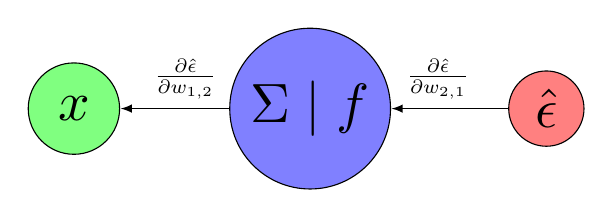
\begin{tikzpicture}[>=latex]

    \path
    (0,0)     node[circle,draw,scale=2,inner sep=2pt,fill=blue!50] (S) {$\Sigma \mid f$}
    +(-3,0)    node[circle,fill=green!50,draw,scale=2]  (x2) {$x$}
    +(0:3)  node[circle,fill=red!50,scale=2,inner sep=2pt,draw]  (y1) {$\hat{\epsilon}$};

\draw[->] (y1)--(S) node[pos=.6,above]{{\color{black}$\frac{\partial \hat{\epsilon}}{\partial w_{2,1}}$}};
\draw[->] (S)--(x2) node[pos=.4,above]{{\color{black}$\frac{\partial \hat{\epsilon}}{\partial w_{1,2}}$}};

\end{tikzpicture}
\end{center}

\end{frame}

\begin{frame}
    \frametitle{Recurrent Neural Network}
    A specific family of ANNs are Recurrent Neural Networks. RNNs are widely used for data with sequential structure. For instance, financial time series data have an intrinsic ordering based along the time dimension. RNNs are endowed with a sequential architecture. This property makes them a good fit for time structured data because the sequential architecture:\vspace{0.25cm}\\
    \begin{itemize}
        \item facilitates sequential signal flow through the neural network.
        \item enables the network to have artificial "memory".
    \end{itemize}
\end{frame}

\begin{frame}
    \frametitle{Recurrent Neural Network}
    \only<1>{RNNs can build up sequential memory due to loops in their architecture. Neurons in hidden layers are not only connected with other neurons but are also connected with themselves, allowing them to loop and store the signal sequentially:\vspace{0.5cm}\\}
    \begin{center}
    \begin{tikzpicture}[>=latex]


        \only<1>{\path
        (0,0)     node[circle,fill=blue!50,draw,scale=1.5] (h1) {$\Sigma \mid f$}
        +(-3,0)    node[circle,fill=green!50,draw,scale=2.1]  (i1) {$x$}
        +(3,0)  node[circle,fill=red!10,draw,scale=1.75]  (y1) {$\hat{y}$};
        \draw[->] (i1)--(h1){};
        \draw[->, dashed] (h1)--(y1){};
        \draw[->, blue] (h1) edge [loop above] node {{\color{black}$\boldsymbol{s_i \rightarrow s_{i+1}}$}} ();}

        \only<2>{\path
        (0,0)     node[circle,fill=blue!50,scale=0,inner sep=1.5pt,draw] (h2) {$f$}
        +(3,0)     node[circle,fill=blue!50,scale=0,inner sep=1.5pt,draw] (h3) {$f$}
        +(-3,0)     node[circle,fill=blue!50,draw] (h1) {$\Sigma \mid f$}
        +(-3,-2.5)    node[circle,fill=green!50,draw]  (i1) {$x_{t-2}$}
        +(0,-2.5)    node[circle,fill=green!50,draw]  (i2) {$x_{t-1}$}
        +(-3,2.5)  node[circle,fill=red!10,draw]  (y1) {$\hat{y}_{1}$}
        +(3,-2.5)    node[circle,fill=green!50,draw,scale=1.4]  (i3) {$x_{t}$};
        \draw[->,red] (i1)--(h1)node[pos=0.5,right]{{\color{black}$\boldsymbol{s_1}$}};
        \draw[->, dashed] (h1)--(y1){};
        \draw[white, thick] (3,2.5) circle(0.5);}



        \only<3>{
        \path
        (0,0)     node[circle,fill=blue!50,draw] (h2) {$\Sigma \mid f$}
        +(3,0)     node[circle,fill=blue!50,scale=0,inner sep=1.5pt,draw] (h3) {$\Sigma \mid f$}
        +(-3,0)     node[circle,fill=blue!50,draw] (h1) {$\Sigma \mid f$}
        +(-3,-2.5)    node[circle,fill=green!50,draw] (i1) {$x_{t-2}$}
        +(-3,2.5)  node[circle,fill=red!10,draw]  (y1) {$\hat{y}_{1}$}
        +(0,-2.5)    node[circle,fill=green!50,draw]  (i2) {$x_{t-1}$}
        +(0,2.5)  node[circle,fill=red!10,draw]  (y2) {$\hat{y}_{2}$}
        +(3,-2.5)    node[circle,fill=green!50,draw,scale=1.4]  (i3) {$x_{t}$};

        \draw[->] (i1)--(h1){};
        \draw[->, dashed] (h1)--(y1){};
        \draw[->,red] (i2)--(h2) node[pos=0.5,right]{{\color{black}$\boldsymbol{s_2}$}}{};
        \draw[->, dashed] (h2)--(y2){};
        \draw[->,blue] (h1)--(h2) node[pos=0.5,above]{{\color{black}$\boldsymbol{s_1 \rightarrow s_2}$}};
        \draw[white, thick] (3,2.5) circle(0.5);

        }

        \only<4>{
        \path
        (0,0)     node[circle,fill=blue!50,draw] (h2) {$\Sigma \mid f$}
        +(3,0)     node[circle,fill=blue!50,draw] (h3) {$\Sigma \mid f$}
        +(-3,0)     node[circle,fill=blue!50,draw] (h1) {$\Sigma \mid f$}
        +(-3,-2.5)    node[circle,fill=green!50,draw]  (i1) {$x_{t-2}$}
        +(-3,2.5)  node[circle,fill=red!10,draw]  (y1) {$\hat{y}_{1}$}
        +(0,-2.5)    node[circle,fill=green!50,draw]  (i2) {$x_{t-1}$}
        +(0,2.5)  node[circle,fill=red!10,draw]  (y2) {$\hat{y}_{2}$}
        +(3,-2.5)    node[circle,fill=green!50,draw,scale=1.4]  (i3) {$x_{t}$}
        +(3,2.5)  node[circle,fill=red!50,draw]  (y3) {$\hat{y}_{3}$};

        \draw[->] (i1)--(h1){};
        \draw[->, dashed] (h1)--(y1){};
        \draw[->] (i2)--(h2){};
        \draw[->, dashed] (h2)--(y2){};
        \draw[->,red] (i3)--(h3)node[pos=0.5,right]{{\color{black}$\boldsymbol{s_3}$}};
        \draw[->] (h3)--(y3){};
        \draw[->] (h1)--(h2){};
        \draw[->,blue] (h2)--(h3)node[pos=0.5,above]{{\color{black}$\boldsymbol{s_2 \rightarrow s_3}$}};
        \draw[white, thick] (3,2.5) circle(0.5);
        }

        \only<5>{
        \path
        (0,0)     node[circle,fill=blue!50,draw] (h2) {$\Sigma \mid f$}
        +(3,0)     node[circle,fill=blue!50,draw] (h3) {$\Sigma \mid f$}
        +(-3,0)     node[circle,fill=blue!50,draw] (h1) {$\Sigma \mid f$}
        +(-3,-2.5)    node[circle,fill=green!50,draw]  (i1) {$x_{t-2}$}
        +(-3,2.5)  node[circle,fill=red!10,draw]  (y1) {$\hat{y}_{1}$}
        +(0,-2.5)    node[circle,fill=green!50,draw]  (i2) {$x_{t-1}$}
        +(0,2.5)  node[circle,fill=red!10,draw]  (y2) {$\hat{y}_{2}$}
        +(3,-2.5)    node[circle,fill=green!50,draw,scale=1.4]  (i3) {$x_{t}$}
        +(3,2.5)  node[circle,fill=red!50,draw]  (y3) {$\hat{y}_{3}$};

        \draw[->] (i1)--(h1){};
        \draw[->, dashed] (h1)--(y1){};
        \draw[->] (i2)--(h2){};
        \draw[->, dashed] (h2)--(y2){};
        \draw[->] (i3)--(h3){};
        \draw[->,blue] (h3)--(y3){};
        \draw[->] (h1)--(h2){};
        \draw[->] (h2)--(h3){};
        \draw[red, thick] (3,2.5) circle(0.5);
        }

        \only<6>{
        \path
        (0,0)       node[circle,fill=blue!50,scale=0,inner sep=1.5pt,draw] (hf) {$\Sigma \mid f$}
        +(-4,0)     node[circle,fill=red!50,scale=0.01,inner sep=2.5pt,draw]  (v) {}
        +(-2,0)     node[circle,fill=red!50,scale=1.5,inner sep=2.5pt,draw]  (y3) {$\hat{y}_{3}$}
        +(4.5,0)      node[circle,fill=red!50,scale=0,inner sep=2.5pt,draw]  (yf) {$\hat{y}$};

        \draw[->,dashed] (v)--(y3){};
        \draw[red, thick] (-2,0) circle(0.8);
            \draw[white, thick] (4.5,0) circle(0.1);
        }

        \only<7>{
        \path
        (0,0)       node[circle,fill=blue!50,scale=1.5,inner sep=1.5pt,draw] (hf) {$\Sigma \mid f$}
        +(-4,0)     node[circle,fill=red!50,scale=0.01,inner sep=2.5pt,draw]  (v) {}
        +(-2,0)     node[circle,fill=red!50,scale=1.5,inner sep=2.5pt,draw]  (y3) {$\hat{y}_{3}$}
        +(4.5,0)      node[circle,fill=red!50,scale=0,inner sep=2.5pt,draw]  (yf) {$\hat{y}$};

        \draw[->,dashed] (v)--(y3){};
        \draw[->] (y3)--(hf){};
        \draw[red, thick] (-2,0) circle(0.8);
        \draw[white, thick] (4.5,0) circle(0.1);
        }

        \only<8>{
        \path
        (0,0)       node[circle,fill=blue!50,scale=1.5,inner sep=1.5pt,draw] (hf) {$\Sigma \mid f$}
        +(-4,0)     node[circle,fill=red!50,scale=0.01,inner sep=2.5pt,draw]  (v) {}
        +(-2,0)     node[circle,fill=red!50,scale=1.5,inner sep=2.5pt,draw]  (y3) {$\hat{y}_{3}$}
        +(3.5,0)      node[circle,fill=red!50,scale=2,draw]  (yf) {$\hat{y}_{t+1}$};

        \draw[->,dashed] (v)--(y3){};
        \draw[->] (y3)--(hf){};
        \draw[->,thick, color=blue] (hf)--(yf)node[pos=.5,above]{final activation};
        \draw[red, thick] (-2,0) circle(0.8);
        \draw[white, thick] (4.5,0) circle(0.1);

        }

\end{tikzpicture}
\end{center}
\end{frame}

\begin{frame}
    \frametitle{RNN Vanishing Gradient Problem}
    In RNNs information is looped sequentially and mixed up with new input information. The amount of initial information quickly diminishes such that after only a few sequences not much of the initial information is left and has little impact on the final output (vanishing gradient problem). In effect, standard RNNs have {\color{ubRed}short memory} and can only take limited advantage of time series' intrinsic structures. There are augmented RNNs that overcome this issue, most prominently:\vspace{0.25cm}\\
    \begin{itemize}
        \item {\color{ubRed}LSTM} (Long Short-Term Memory)
        \item {\color{ubRed}GRU} (Gated Recurrent Unit)

    \end{itemize}

\end{frame}

\begin{frame}
    \frametitle{Reinforcement Learning}

\begin{center}
    \animategraphics[loop,autoplay,width=10cm]{10}{Mario/mario-}{0}{99}
\end{center}
\end{frame}

\begin{frame}
    \frametitle{Reinforcement Learning}
Reinforcement Learning (RL) is a framework to model the {\color{ubRed}decision making process}:\vspace{0.25cm}\\
\begin{itemize}

\item of an {\color{ubRed}agent},
\item in a {\color{ubRed}environment} with a sequence of possible {\color{ubRed}states}, $s_t$,
\item in order to maxmize a sequence of {\color{ubRed}rewards}, $r$.\vspace{0.25cm}\\
\end{itemize}

 Reinforcement learning does not necessarily need labelled input and output variables. Rather, a RL problem is typically stated in the form of a {\color{ubRed}Markov decision process} (MDP) and uses {\color{ubRed}dynamic programming} techniques:\vspace{0.25cm}\\
 \begin{itemize}

 \item  to find the {\color{ubRed}optimal action}, $a$, to be taken,
 \item given some state, $s_t$,
 \item in order to {\color{ubRed}maximize some notion of cumulative reward} (final value), $V$.\vspace{0.25cm}\\
 \end{itemize}  The rule that assigns a given state to the best possible action is called {\color{ubRed}policy}, $\Pi(\theta, a)$, and is learned using some ML technique such as neural networks.
\end{frame}

\begin{frame}[fragile]
    \frametitle{Deep Reinforcement Learning}
    \begin{center}
        \tikzset{
           neuron missing/.style={
            draw=none,
            scale=0.5,
            text height=0.333cm,
            execute at begin node=\color{black}$\vdots$
          },
        }

        \newcommand{\DrawNeuronalNetwork}[2][]{
        \xdef\Xmax{0}
        \foreach \Layer/\X/\Col/\Miss/\Lab/\Count/\Content [count=\Y] in {#2}
        {\pgfmathsetmacro{\Xmax}{max(\X,\Xmax)}
         \xdef\Xmax{\Xmax}
         \xdef\Ymax{\Y}
        }
        \foreach \Layer/\X/\Col/\Miss/\Lab/\Count/\Content [count=\Y] in {#2}
        {\node[anchor=south] at ({2*\Y},{\Xmax/2+0.1}) {\Layer};
         \foreach \m in {1,...,\X}
         {
          \ifnum\m=\Miss
           \node [neuron missing] (neuron-\Y-\m) at ({2*\Y},{\X/2-\m}) {};
          \else
           \node [circle,fill=\Col!50,minimum size=0.4cm,draw] (neuron-\Y-\m) at
          ({2*\Y},{\X/2-\m}) {\Content};
         \ifnum\Y=1
          \else
           \pgfmathtruncatemacro{\LastY}{\Y-1}
           \foreach \Z in {1,...,\LastX}
           {
            \ifnum\Z=\LastMiss
            \else
             \draw[->] (neuron-\LastY-\Z) -- (neuron-\Y-\m);
            \fi
            }
          \fi
         \fi
         \ifnum\Y=1
          \ifnum\m=\X
           \draw [overlay] (neuron-\Y-\m) -- (state);
          \else
           \ifnum\m=\Miss
           \else
            \draw [overlay] (neuron-\Y-\m) -- (state);
           \fi
          \fi
         \else
         \fi
         }
         \xdef\LastMiss{\Miss}
         \xdef\LastX{\X}
        }
        }
        \begin{tikzpicture}[x=0.75cm, y=0.5cm,
        >=stealth,font=\sffamily,nodes={align=center}]
         \begin{scope}[local bounding box=T]
          \path  node[draw,minimum width=6em,minimum height=4em] (state) {State};
          \begin{scope}[local bounding box=NN]
           \DrawNeuronalNetwork{\scriptsize{Input Layer}/5/green/4///,
             \scriptsize{Hidden Layer}/5/blue/4//11/,
             \scriptsize{Output Layer}/4/red/3//11/}
          \end{scope}
          \path (NN.south) node[below]{Estimated parameter\\ $\theta$};
          \path(NN.east) -- node[above]{Policy\\ $\Pi(\theta,a)$}++ (4em,0);
         \end{scope}
         \node[fit=(T),label={[anchor=north west]north west:Agent},inner sep=1em,draw]
          (TF){};
         \node[below=3em of TF,draw,inner sep=1em] (Env) {Environment};
         \draw[<-] (TF.200) -- ++ (-1em,0) |- (Env.160) node[pos=0.45,right]{$r_t$};
         \draw[<-] (TF.180) -- ++ (-2em,0) |- (Env.180) node[pos=0.45,left]{$s_t$};
         \draw[->] (NN.east) -- ++ (7em,0)node[right]{$a_t$} |- (Env);
        \end{tikzpicture}
\end{center}
\end{frame}

\begin{frame}

    \frametitle{Optimal Managerial Decision}
    \textbf{Example 1: Optimal managerial decision}\vspace{0.5cm}\\
    Assume that the firm value for shareholders is the amount of all future cash flows which are distributed to them. The distributions are defined using following accounting identity (a simplified model of \cite{Nikolov2014}):
    \begin{align}
    d(k,k',\epsilon) \equiv (1-\tau)\epsilon k^{\theta} + \delta k \tau - I - \Psi(I,k) + f(1-\phi),
\end{align}
    where the first two terms represent after-tax operating profits, the second and third term account for cash outflows due to an investment and its cost, and the last term captures any outside financing that can be used to distribute value to shareholders. Furthermore, assume that the manager acts in the shareholder's best interest.
\end{frame}

\begin{frame}
    \frametitle{Optimal Managerial Decision}
    The manager {\color{ubRed}chooses the capital stock}, $k$, through investment, $i$,  each period to maximize the present value of the firm, that is, all future distribution to shareholders. The corresponding Bellman equation for the problem is then:
    \begin{align}
    V(k,\epsilon) ={\max\limits_{k'}} \Bigl\{ d(k,k',\epsilon)  + \frac{1}{1+r} \int  V(k,'\epsilon')   dq(\epsilon',\epsilon)      \Bigr\}
\end{align}
The policy assigns the optimal investment behaviour to a given state of the environment (characterized by innovations/shocks, $\epsilon$) in order to maximise the capital stock in the long term.
\end{frame}

\begin{frame}
    \frametitle{Intertemporal Asset Allocation}
    \textbf{Example 2: Intertemporal asset allocation}\vspace{0.5cm}\\
    Assume that investors seek to maximize expected ``lifetime'' utility over consumption $C_t$ and bequest $W_T$:
    \begin{align}
      \mathbb{E}\left[\sum_{t=0}^{T-1}u(C_t,t)+F(W_T)\right]
  \end{align}
      Where:\vspace{0.25cm}\\
      \begin{itemize}
      \item $F$ is increasing and concave
      \item $u$ is continuous in $c$ and $t$ and increasing and concave in $c$. Further assume that either $u$ or $F$ is strictly concave\vspace{0.25cm}\\
      \end{itemize}
Furthermore, the investors' information set is generated by a vector $\mathbf{X}_t$ of $K$ state variables.
\end{frame}

\begin{frame}
    \frametitle{Intertemporal Asset Allocation}

  	Suppose that at date $t$ an investor has wealth $W_t$. She can choose to consume $C_t$ out of it, which leaves her with $W_t-C_t$ to invest. She can invest fractions $\mathbf{w}_t$ of this amount in the $N$ risky assets and the remaining fraction $1-\mathbf{w}_t'\mathbf{1}$ in the riskless account at rate $r_{f,t}$. Hence, her wealth next period will be:
    \begin{align}
  	W_{t+1}&=(W_t-C_t)\underbrace{(\mathbf{w}_t'(\mathbf{r}_{t+1}-r_{f,t+1}\mathbf{1})+r_{f,t+1})}_{\equiv r_{p,t+1}}
\end{align}

For convenience, denote the set of budget-feasible strategies by $\mathscr{S}(\mathbf{X}_t)$. Putting everything together the investor's problem is to {\color{ubRed} find the policy, i.e., choose a sequence of vectors of weights} $\{\mathbf{w}_t\}_{t=0}^{T-1}$ and a {\color{ubRed}sequence of consumptions} $\{C_t\}_{t=0}^{T-1}$, to maximize her lifetime expected utility:\begin{align}
  	&\max_{\{\mathbf{w}_t\}_{t=0}^{T-1},\{C_t\}_{t=0}^{T-1}}\mathbb{E}\left[\sum_{t=0}^{T-1}u(C_t,t)+F(W_T)\right]\\
  	&\text{subject to }\begin{array}{c c c}(\mathbf{w}_t,C_t)\in\mathscr{S}(\mathbf{X}_t), & \mathbf{X}_{t+1}=L(\mathbf{X}_{t}) & \forall t\in\{0,...,T-1\}\notag\end{array}
\end{align}
\end{frame}

\begin{frame}
    \frametitle{Finding the Optimal Policy}
    In both of the above settings one could use reinforcement learning to obtain the {\color{ubRed}optimal policy}:\vspace{0.25cm}\\
    \begin{itemize}
        \item the manager who chooses how much to invest each period in order to maximize firm value, depending on the state of the environment (investment opportunities).
        \item the investor choosing the optimal trading/investment strategy in order to maximize her wealth, for instance, by rotating between value, size, and momentum strategies, or by switching between active and passive investing, depending on the state of the market environment.
    \end{itemize}
\end{frame}


\begin{frame}
    \frametitle{Preprocessing - Data Samples}
    The performance of a neural network can only be evaluated when cast on data it has never seen before. Therefore, it is required that the data be split into two sets:\vspace{0.25cm}\\
    \begin{itemize}
        \item {\textbf{\color{ubRed}Taining set}:} A subset, $A$, of the original data from which the neural network learns (in-sample).
        \item {\textbf{\color{ubRed}Validation set}:} A subset, $B$, of the original data to asses whether the neural network produces a good fit for data it has not seen before (out-of-sample).
        \item The two subsets have no common observations, i.e., $\{A\} \cap \{B\} = \emptyset$ \vspace{0.25cm}\\
    \end{itemize}
    For time series data one must additionally specify a:\vspace{0.25cm}\\
    \begin{itemize}
        \item {\textbf{\color{ubRed}Data window}:} A chronological sequence of input variables from which one future observation is predicted. \vspace{0.25cm}\\
    \end{itemize}
 Most observations of the original data should be assigned to the training set while only a minority of observations should be assigned to the validation set, for instance, 90\%/10\%. A good neural network produces a good fit, i.e., a small error, for both sets. Partitioning your data into a training and validation set is the simplest form of {\color{ubRed} cross-validation}.\\
\end{frame}



\begin{frame}
    \frametitle{Preprocessing - Input Variables}
Most of the times, your dataset will contain input variables highly varying in magnitudes, units and range. But since, many machine learning algorithms use a distance based error measure, this is a problem. Hence, it is of towering importance that the input data be standardized in some way:\vspace{0.25cm}\\
\begin{itemize}
    \item {\textbf{\color{ubRed}Standardization}:} Standardize the values to have a zero mean and unit variance
    \item {\textbf{\color{ubRed}Normalization}:} Rescale the values to a domain of $[0,1]$
    \item The data is naturally homogeneous
\end{itemize}
\vfill
\begin{exampleblock}{{\small{Command}}}
In \texttt{Python} standardizing variables is facilitated using sklearn.preprocessing.\href{https://scikit-learn.org/stable/modules/generated/sklearn.preprocessing.StandardScaler.html}{\color{Purple}StandardScaler}, while normalizing variables is facilitated using sklearn.preprocessing.\href{https://scikit-learn.org/stable/modules/generated/sklearn.preprocessing.normalize.html}{\color{Purple}normalize}
\end{exampleblock}

\end{frame}


\begin{frame}
    \frametitle{Preprocessing - Labelling}
    In some cases one might be interested into classifying time series observations into classes and assign {\color{ubRed}labels}. Following \cite{DePrado2018}, the following labelling schemes are especially suited for returns:\vspace{0.25cm}\\
    \begin{itemize}
        \item {\textbf{\color{ubRed}Binary encoding}:} Assigning a value of 1 to positive returns, and 0 otherwise.
        \item {\textbf{\color{ubRed}Quantile encoding}:} Assigning return observations to a specified number of quantiles.
        \item {\textbf{\color{ubRed}Sigma encoding}:} Rather than prespecifying the number of possible quantiles, sigma encoding lets the return stream decide the set of values and uses the standard deviation to discretize the return sequence. The number of values in the set is defined by $\left\lceil \frac{max\{r\} - min\{r\}}{\sigma}\right\rceil$ and each return is assigned to a value according to $\left\lfloor \frac{r_t - min\{r\}}{\sigma}\right\rfloor$. In effect, we assign 0 to $r_t \in \left[min\{r\},min\{r\}+\sigma\right)$, 1 to $r_t \in \left[min\{r\}+\sigma,min\{r\}+2\sigma\right)$, and so on.
    \end{itemize}
\end{frame}

\begin{frame}
    \frametitle{Preprocessing - Data Shuffling}
It is important that the training data is shuffled, i.e., it comes in a non-specific, random order. Elsewise, the neural network is subject to learning an order that does not arise from the data itself (ascending order, alphabetical, etc.) This even pertains to time series with intrinsic ordering. However, this does not mean that the time series observations itself should be shuffled. Rather, it means that one should feed the {\color{ubRed}data windows} in a random pattern:\vspace{0.5cm}\\

\begin{table}[t]
\centering
\textbf{1.} \begin{tabular}{|c|c|c|c|}
\hline
25.03 & 26.03 & 27.03 & 28.03\\
\hline
 {\color{green!50}$x_{t-2}$} & {\color{green!50}$x_{t-1}$} & {\color{green!50}$x_{t}$} & {\color{red!50}$\hat{y}_{t+1}$}\\
\hline
\end{tabular}
\hspace{0.25cm}$\longrightarrow$\hspace{0.25cm}
\textbf{1.} \begin{tabular}{|c|c|c|c|}
\hline
25.03 & 26.03 & 27.03 & 28.03\\
\hline
 {\color{green!50}$x_{t-2}$} & {\color{green!50}$x_{t-1}$} & {\color{green!50}$x_{t}$} & {\color{red!50}$\hat{y}_{t+1}$}\\
\hline
\end{tabular}
\end{table}

\begin{table}[t]
\centering
\textbf{2.} \begin{tabular}{|c|c|c|c|}
\hline
 26.03 & 27.03 & 28.03 & 29.03\\
\hline
 {\color{green!50}$x_{t-2}$} & {\color{green!50}$x_{t-1}$} & {\color{green!50}$x_{t}$} & {\color{red!50}$\hat{y}_{t+1}$}\\
\hline
\end{tabular}
\hspace{0.25cm}$\longrightarrow$\hspace{0.25cm}
\textbf{2.} \begin{tabular}{|c|c|c|c|}
\hline
11.08 & 12.08 & 13.08 & 14.08\\
\hline
 {\color{green!50}$x_{t-2}$} & {\color{green!50}$x_{t-1}$} & {\color{green!50}$x_{t}$} & {\color{red!50}$\hat{y}_{t+1}$}\\
\hline
\end{tabular}
\end{table}



\begin{table}[t]
\centering
\textbf{3.} \begin{tabular}{|c|c|c|c|}
\hline
 27.03 & 28.03 & 29.03 & 30.03\\
\hline
 {\color{green!50}$x_{t-2}$} & {\color{green!50}$x_{t-1}$} & {\color{green!50}$x_{t}$} & {\color{red!50}$\hat{y}_{t+1}$}\\
\hline
\end{tabular}
\hspace{0.25cm}$\longrightarrow$\hspace{0.25cm}
\textbf{3.} \begin{tabular}{|c|c|c|c|}
\hline
05.05 & 06.05 & 07.05 & 08.05\\
\hline
 {\color{green!50}$x_{t-2}$} & {\color{green!50}$x_{t-1}$} & {\color{green!50}$x_{t}$} & {\color{red!50}$\hat{y}_{t+1}$}\\
\hline
\end{tabular}
\end{table}
\begin{center}
    $\vdots$
\end{center}

\end{frame}

\begin{frame}
    \frametitle{Preprocessing - Class Weights}
    Another issue often encountered in machine learning are {\color{ubRed}imbalanced datasets}. This means that a certain value of a variable is represented much more often in the data sample than other values of the same variable. Depending on the question at hand, this can become a substantial issue. One remedy are {\color{ubRed} class weights}.\vspace{0.25cm}\\
    \begin{itemize}
    \item Class weights specify that a certain realization of a variable should have more weight when training neural networks than other variables.
    \item  This is achieved by giving them more weighted impact on the fitting error such that they cannot be neglected just because they are rare.\vspace{0.25cm}\\
\end{itemize}
    For instance, if $x_1$ is represented twice as much as $x_2$, then $x_2$ should have a class weight of $2/3$ and $x_1$ a class weight of $1/3$.
    \vfill
    \begin{exampleblock}{{\small{Command}}}
    In \texttt{Python}  adding class weights is an option in the model fitter command in Tensorflow and Keras. It is implemented using model.fit(...,\href{https://keras.io/models/model/\#fit}{\color{Purple}class\_weight}=$\{$class\_weight\_dictionary$\}$,...).
    \end{exampleblock}
\end{frame}

\begin{frame}
    \frametitle{Preprocessing - Stationarity vs. Memory}
    What makes time series non-stationary is {\color{ubRed}memory}, the presence of a long history of previous levels that shift the series mean over time.\vspace{0.25cm}\\
    \begin{itemize}
        \item Taking returns undoubtedly renders a time series stationary.
        \item This happens at the cost of erasing all its memory.
        \item Being able to exploit memory in time series is a powerful ability found in some ML algorithms .\vspace{0.25cm}\\
    \end{itemize}

 Hence, one should desire to give up only so much memory such that the time series becomes stationary while keeping as much memory as possible at the same time. To that end, \cite{DePrado2018} suggests {\color{ubRed}fractional differencing}, which allows the order of integration to take on any real positive number and not only integers, and idea that dates back at least to \cite{Hosking1981}.
\end{frame}


\begin{frame}
    \frametitle{Preprocessing - Stationarity vs. Memory}
    Formally, using a lag operator $L$ applied to a time series $\{x_t\}$ we have that $x_{t-k} = L^kx_t$ for any integer satisfying $k\geq 0$, where $k$ denotes the order of lag. For example, $(1-L)^2 = 1-2L + L^2$, so that $(1-L)^2x_t = x_t - 2x_{t-1} + x_{t-2}$. From the fact that:
    \begin{align}
    (a + b)^n = \sum\limits_{k=0}^n \binom{n}{k} a^{n-k}b^k,
    \end{align}
    it follows that for any real number $d$ we have:
    \begin{align}
    (1 + b)^d = \sum\limits_{k=0}^{\infty} \binom{d}{k} b^k, \label{binomialcoeff}
    \end{align}
    the binomial series.
\end{frame}

\begin{frame}
    \frametitle{Preprocessing - Stationarity vs. Memory}
     In order to achieve a fractional model we map \eqref{binomialcoeff} onto our lag operator and allow for $d$ to be any real number and use the following binomial series expansion:
    \begin{align}
    	(1-L)^d = \sum\limits_{k=0}^{\infty} \binom{d}{k} (-L)^k &= \sum\limits_{k=0}^{\infty} (-L)^k \prod\limits_{i=0}^{k-1}\frac{d-i}{k-i} \notag \\
    	&=  \sum\limits_{k=0}^{\infty} (-L)^k \frac{\prod_{i=0}^{k-1}(d-i)}{k!} \notag \\
    	&= 1 -dL + \frac{d(d-1)}{2!}L^2 - \frac{d(d-1)(d-2)}{3!}L^3 + \hdots \label{getweights}
    \end{align}
\end{frame}
\begin{frame}
    \frametitle{Preprocessing - Stationarity vs. Memory}
    If we have a time series $\{x_t\}$ we can transform it into a fractionally differentiated time series of order $d$ by defining it as a dot product of realizations of $\{x_t\}$ and weights $w_k$ obtained from the binomial series expansion in equation \eqref{getweights} such that:
    \begin{align}
     \{\tilde{x}_t^d\} &= \left\{\sum\limits_{k=0}^{\infty}w_kx_{t-k}, \sum\limits_{k=0}^{\infty}w_kx_{t-1-k}, \hdots, \sum\limits_{k=0}^{\infty}w_kx_{t-l-k}\right\}
 \end{align}
    where $\{\tilde{x}_t^d\}$ denotes the fractionally differentiated time series of $\{x_t\}$ with order $d$ and where the weight vector correspond to:
    \begin{align}
    	\boldsymbol{w} = \left\{ 1, -d, \frac{d(d-1)}{2!}, -\frac{d(d-1)(d-2)}{3!}, \hdots, (-1)^k\prod\limits_{i=0}^{k-1}\frac{d-i}{k!} \right\} \label{fracweights}
    \end{align}
    \end{frame}

    \begin{frame}
        \frametitle{Preprocessing - Stationarity vs. Memory}
    When $d$ is a positive integer, the memory beyond that point is purged since $\prod_{i=0}^{k-1}\frac{d-i}{k!} =0, \forall k > d$. If the time series $\{x_t\}$ are log prices, when setting $d$ to one it becomes obvious from equation \eqref{fracweights} that the resulting weights are $w = \{1,-1,0,0,\hdots\}$ and in effect, the time series maps to a series of log returns, $(1-L)x_t = x_t - Lx_t = x_t - x_{t-1}$, where all memory beyond a lag of one vanishes. In order to find the {\color{ubRed}optimal order of differencing}, one can gradually increase the order until the augmented Dickey-Fuller test rejects the null hypothesis of non-stationarity.\vspace{0.25cm}\\

\begin{itemize}
    \item \cite{DePrado2018} finds that  {\color{ubRed}many securities are stationary when $d$ is between 0.3 and 0.6} which seems to imply that taking standard returns casts away valuable memory of the time series.
\end{itemize}
\vfill
The augmented Dickey-Fuller test can be revisited here:  \hyperlink{Dickey}{\beamergotobutton{Augmented Dickey-Fuller test}}
        \end{frame}

       \begin{frame}
            \frametitle{Overfitting and Cross-validation}
              A model is said to be {\color{ubRed}overfit} when it performs well in-sample but performs poorly out-of-sample. The discrepancy between in-sample and out-of-sample performance is known as generalization error. Specifically, an error estimation, $\hat{\epsilon}$, is made for the model when training. However, this only gives us an idea about how well our model does on data used to train it. The problem with evaluating this training error is that it does not give an indication of how well the model will generalize to an independent and unseen data set. Evaluating whether the model performs well on unseen data is known as {\color{ubRed}cross-validation}. Popular cross-validation approaches are:\vspace{0.25cm}\\
             \begin{itemize}
                     \item {\textbf{\color{ubRed}Holdout method}:} Splitting the data into a training and validation set.
                     \item {\textbf{\color{ubRed}K-Fold cross-validation}:} The data is divided into $K$ equally sized subsets. Now, the holdout method is repeated $K$ times, such that each time, one of the $K$ subsets is used as the validation set and the other $K-1$ subsets form the training set.
                     \item {\textbf{\color{ubRed}Repeated random sub-sampling}:} Similar to K-fold cross-validation, but this time in each training iteration a random fraction of observations in the dataset are randomly set aside for training. \vspace{0.25cm}\\
             \end{itemize}
        \end{frame}

        \begin{frame}
            \frametitle{Reading Tip}
        López de Prado, M. (2018), Advances in Financial Machine Learning, Wiley\vspace{0.35cm}\\
        \begin{center}

            \includegraphics[scale=0.85]{DePrado}
        \end{center}
        \end{frame}

%         \begin{frame}[label=Crypto]
%             \begin{center}
%                 {\color{ubRed} \Huge{Cryptocurrencies and Mathematics for Cryptos}}
%             \end{center}
%         \end{frame}
%
%
%         \begin{frame}
%             \frametitle{Centralized System of Payment}
%             Usual system of payment:
%             \begin{itemize}
%                 \item centralized
%                 \item clearing at the end of the day: internally transfer amounts between accounts
%
%             \end{itemize}
%             \begin{center}
%             \includegraphics[scale=0.2]{centralized.png}
%         \end{center}
%         \end{frame}
%
%         \begin{frame}
%             \frametitle{Centralized System of Payment}
%             Interbank setting:
%             \begin{itemize}
%                 \item centralized
%                 \item clearing at the end of the day: first internally transfer amounts between accounts at the same bank then net interbank
%
%             \end{itemize}
%             \begin{center}
%             \includegraphics[scale=0.2]{interbank.png}
%         \end{center}
%         \end{frame}
%
%         \begin{frame}
%             \frametitle{Centralized System of Payment: Example}
%             Interbank setting:
%             \begin{itemize}
%                 \item Clearing at the end of day:
%                 \begin{itemize}
%                     \item internally transfer amounts between accounts
%                     \item amount UBS owes to CS; ex: 10
%                     \item amount CS owes to UBS; ex: 11
%                 \end{itemize}
%                 \item CS can borrow 1 from UBS in interbank market overnight
%                 \item CS can borrow 1 from central bank
%                 \item CS can transfer 1 to UBS using its deposit at central Bank
%                 \item One party could default
%             \end{itemize}
%
%         \end{frame}
%
%         \begin{frame}
%             \frametitle{Mistrust in the System}
%
%             \begin{itemize}
%                 \item Mistrust in government authorities, monetary policy, and financial markets
%                 \item Banks where money is deposited may default
%                 \item Corruption, disappropriation
%                 \item Payment system (SWIFT) may be taken hostage
%                 \item need a way to launder and hide money of criminal origin :)
%             \end{itemize}
%
%         \end{frame}
%
%         \begin{frame}
%             \frametitle{Decentralized Network}
%             Potentially every node can be connected with each other
%
%             \begin{center}
%             \includegraphics[scale=0.25]{decentralized.png}
%         \end{center}
%         \end{frame}
%
%         \begin{frame}
%             \frametitle{Decentralized Network}
%             Some characteristics of a decentralized payment system are:
%             \begin{itemize}
%                 \item Transactions are transparent such that everybody can verify
%                 \item Everybody can hold a copy of the entire network history
%                 \item If a part of the network disappears the remaining network can continue
%                 \item A transactions an never be cancelled as long as ledger exists
%                 \item A committee decides on future
%                 \item Minimal frontiers: worldwide currency
%             \end{itemize}
%         \end{frame}
%
%         \begin{frame}
%             \frametitle{Transaction: Theory}
%             This is a rough sketch of what a Bitcoin transaction in a decentzralized network looks like:
%             \begin{itemize}
%                 \item Suppose Alice wants to send some BTC to Bob. She asks Bob for an address in his wallet which he will convey by EMail or some application
%                 \item Alice will use her \textbf{client}, i.e. program on her computer to take some units of bitcoin from her own \textbf{electronic wallet} and send them to Bob
%                 \item Alice's client takes information about where money comes from and where it goes and broadcasts to network
%                 \item Electronic wallet can be on home computer or located with an exchange
%                 \item Transactions specifies how remaining bitcoins (like small change) should be split between miner and herself
%                 \item Miners then grab transaction (or not) and start mining
%             \end{itemize}
%         \end{frame}
%
%         \begin{frame}
%             \frametitle{Transaction: Illustration}
%             \begin{center}
%                 \includegraphics[scale=0.4]{transaction.png}
%             \end{center}
%             \begin{itemize}
%                 \item A transaction where Alice pays 7 BTC to Bob using various sources
%                 \item Alice uses previous transactions where a total to 8 BTC were sent to her
%                 \item The remainder of 0.5 is the fee of the miner
%                 \item Unlike bank, there is no balance of Alice's account
%             \end{itemize}
%         \end{frame}
%
%         \begin{frame}
%             \frametitle{Mining: Theory}
%             Each time a transaction gets broadcast all miners in the network can:
%             \begin{itemize}
%                 \item Verify the validity of the transaction:
%                 \begin{itemize}
%                 \item Did Alice receive the coins she claims to have?
%                 \item From which block/transaction Alice got the coins
%                 \item Did Alice already spend those coins? Double spending problem
%                 \item Info on spent transactions is available from the net
%                 \end{itemize}
% 				\item Include the transaction in a new block
% 				\item Solve a mathematical puzzle which can be easily verified but which is taking time and is \textbf{costly}
%             \end{itemize}
%             Mining results in {\color{ubRed} Proof of Work}
%         \end{frame}
%
%
%         \begin{frame}
%             \frametitle{Mining: Limitations}
%             Some problems/limitations of Bitcoin mining are:
%             \begin{itemize}
%                 \item Block size is limited to 1MB (one mega byte)
%                 \item Expect miner to grab most interesting transactions (low validation cost, high fee)
%                 \item The solution of the puzzle has a difficulty level so that on average a
% block can be mined (validated) every 10 minutes
%                 \item It results that in 10 minutes, Bitcoin processes transactions at an average rate of 7/sec (Visa 10'000/sec)
%                 \item The difficulty of the puzzle is adjusted every 2016 blocks based on the time it took to find the previous 2016 blocks
%                 \item Since a hostile miner could incorporate invalid transactions, only after
% successful mining of 6 blocks there is consensus and the miner can get his fee and additional Bitcoins (as long as new Bitcoins will be generated).
%
%             \end{itemize}
%         \end{frame}
%
%  \begin{frame}
%  \frametitle{Problems with Bitcoin}
%  \begin{itemize}
%  \item Speed by which transactions are incorporated (if they are) in blocks is too slow. 10 minutes before a transaction is validated for the first time. It may take up to an hour before consensus (6 consecutive blocks are validated). And blocksize is limited to 1MB
%  \item Bitcoin processes transactions at an average rate of 7/sec vs. 10'000/sec processed by credit cards
%  \item Bitcoin transactions cannot be taken back. The only way to undo a transaction is to convince counterpart to create a new reversing transaction. There is no authority to enforce this
%  \item Exchange FIAT money against Bitcoins and vice-versa.
%  \begin{itemize}
%  \item Interface is potentially unsecured and wallet may get erased or credentials are lost
%  \item Exchanges have been broken in
%  \end{itemize}
%
%  \item Bitcoin does not allow storage of notary documents, other currencies allow storage/exchange of any information.
%  \item Bitcoin encourages speculation. Naive (Stupid) individuals may want to participate in Bitcoin and lose their wealth.
%  \item More than 4000 crypto currencies available (January 2021) . Which one will survive?
%  \item {\color{ubRed} Economic foundations?}
%  \end{itemize}
% \end{frame}
%
% \begin{frame}
% \frametitle{Bitcoin's Biggest Problem}
% Economic foundation:
% \begin{itemize}
% \item {\color{ubRed} Someone actually needs to keep the network running!} The network operates as long as there are miners that profit from validating transactions: \begin{align}
% \text{Profit} = \underbrace{\text{Bitcoins mined}}_{\rightarrow 0 }  + \text{transaction fees} - \text{energy cost} - \text{infrastructure costs}
% \end{align}
% \begin{itemize}
% \item Bitcoin emission is limited to 21 million. Then only incentive in the long term is fee
% \item Bitcoin premiss is that {\color{ubRed} there will be a sufficiently large pool of individuals willing to pay transactions}
% \end{itemize}
% \item Why should such a pool of individuals exist?
% \item Bitcoin is inefficient (few transactions/sec). Only those transaction with highest fees will be selected by miners.
% \end{itemize}
% \textbf{Conclusion:} Bitcoin in its present form is not sustainable and in a rational expectation model its value in the long term is zero
% \end{frame}
%
%
% \begin{frame}
% \frametitle{Rational Expectations Equilibrium}
%
% In a Rational Expectations Equilibrium, if BTC has zero value at some point, yet current prices are positive, this must mean that:
% \begin{itemize}
% \item There will be a hard fork in the future where a part of the Bitcoin network splits into something better
% \item or we need to appeal to behavioural  economics
% \end{itemize}
% If the rational expectation is that Bitcoin will fork into something better at some point, then why not  pick up a better and more sustainable crypto-currency now? Behavioural economics more likely to explain the positive price
% \end{frame}
%
% \begin{frame}
% \frametitle{Behavioural Economic Model}
% Bitcoin price is likely driven by behavioural patterns:\vspace{0.25cm}\\
% \begin{itemize}
% \item Bitcoin has become a {\color{ubRed} religion}. People blindly follow recommendations of high profile individuals
% \item Individuals try to mobilize as many other people as possible to invest into Bitcoin highlighting some potential future value, e.g., through social media while flaunting some crazy lifestyle.
% \item Many financially illiterate investors invest due to {\color{ubRed} FOMO} creating buying pressure
% \item Rallies are fuelled by incredibly high - and maybe absurd - price targets from random sources: \emph{"If all people store their wealth in Bitcoin one Bitcoin coud be worth X million"}. This can lead to severe confirmation bias and increase FOMO and buying pressure even further.
% \item Eventually institutional investors try to game the market by applying momentum strategies and increase buying pressure even further.\vspace{0.25cm}\\
% \end{itemize}
% This speculative game can have severe downward consequences for those who are at the bottom of that "pyramid"
% \end{frame}


        \begin{frame}
            \begin{center}
                {\Huge{{\color{ubRed}Bibliography}}}
            \end{center}
        \end{frame}

        \begin{frame}[allowframebreaks]
        \frametitle{References}
        \bibliography{Buybacks}
\end{frame}

\appendix
        \begin{frame}
            \begin{center}
                {\Huge{{\color{ubRed}Appendix}}}
            \end{center}
        \end{frame}



\begin{frame}[label=Event_studies]
    \frametitle{Event-Studies}
    An event study measures the effect of some company-specific information (usually the
announcement of a corporate decision) on the prices of stocks of the company.\vspace{0.25cm}\\
Event studies are tests of market efficiency. If abnormal returns after the
announcement are significantly different from zero, markets are not semi strong
efficient. Hence, through event studies, we can check for profitable trading strategies.\vspace{0.25cm}\\
If the market is efficient, event studies allow estimating the economic impact of
corporate decisions. We care about the “average” response to announcements, not the
response to some specific company’s announcement.\vspace{0.25cm}\\
Corporate decisions have been the focus of lots of event studies (mainly in the US):\vspace{0.25cm}\\
\begin{itemize}
    \item earnings announcement
    \item IPOs
    \item share repurchases
    \item M\&A
    \item etc.
\end{itemize}
\end{frame}

\begin{frame}
    \frametitle{Event-Studies}
    \textbf{General procedure}\vspace{0.25cm}\\
    \begin{enumerate}[1.]
        \item Find a sample of firms that have announced the same news (event) in the past
        \item Define time $\tau = 0$ as the {\color{ubRed} event date}, i.e. the announcement in a widely disseminated
publication
\item Define the windows useful for the analysis\vspace{0.25cm} around the event date\\
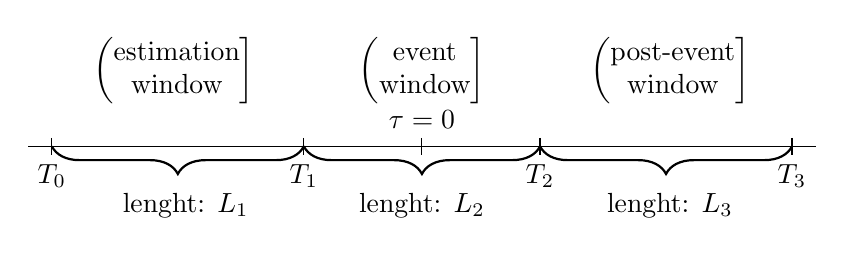
\begin{tikzpicture}
    \draw (0.5,0) -- (10.5,0);
    \foreach \x in {0.8,4,5.5,7,10.2}
    \draw(\x cm,3pt) -- (\x cm, -3pt);
    \draw (0.8,0) node[below=3pt] {$T_0$};
    \node[align=center] at (2.5,-0.75) {lenght: $L_1$};
    \draw [thick,decorate,decoration={brace,amplitude=10pt,raise=0pt,mirror}] (0.8,0) -- (4,0);
    \draw (4,0) node[below=3pt] {$T_1$};
    \draw (5.5,0) node[above=3pt] {$\tau = 0$};
    \node[align=center] at (5.5,-0.75) {lenght: $L_2$};
    \draw [thick,decorate,decoration={brace,amplitude=10pt,raise=0pt,mirror}] (4,0) -- (7,0);
    \draw (7,0) node[below=3pt] {$T_2$};
    \node[align=center] at (8.65,-0.75) {lenght: $L_3$};
    \draw [thick,decorate,decoration={brace,amplitude=10pt,raise=0pt,mirror}] (7,0) -- (10.2,0);
    \draw (10.2,0) node[below=3pt] {$T_3$};
    \draw (2.35,0) node[above=12pt, align=center] {
                            $\left(\mytab{estimation \\ window}\right]$};
                            \draw (5.5,0) node[above=12pt, align=center]{
                            $\left(\mytab{event \\ window}\right]$};
                            \draw(8.65,0) node[above=12pt, align=center]{
                            $\left(\mytab{post-event \\ window}\right]$};
    \end{tikzpicture}

    \item Over the {\color{ubRed}estimation window}, estimate the parameters of the normal return model. $\E[r_{i,t}]$ is the normal return that the stock would experienced if there were no event
    \end{enumerate}

\end{frame}

\begin{frame}[label=event_studies_main]
    \frametitle{Event-Studies}
    \begin{enumerate}[5.]
        \item Over the  {\color{ubRed}event window}, estimate the series of abnormal returns $\forall i, i\in N$:
        \begin{align}
            AR_{i,t} = r_{i,t} - \E[r_{i,t}] \text{, \hspace{1cm} for } t=T_1+1, \hdots, T_2
        \end{align}
        \item[6.] Compute, on each day in the event window, the average abnormal return across all
N firms in the sample
\begin{align}
    AAR_{t} = \frac{1}{N}\sum\limits_{i=1}^N AR_{i,t} \text{, \hspace{1cm} for } t=T_1+1, \hdots, T_2
\end{align}
\item[7.] Compute the  {\color{ubRed} Cumulative Average Abnormal Return} (CAAR)
\begin{align}
    CAAR_{t} = \sum\limits_{t=T_1+1}^{T_{2}} AAR_t \text{, \hspace{1cm} for } t=T_1+1, \hdots, T_2
\end{align}
\item[8.] Test for statistical significance and interpret the results\vspace{0.25cm}\\
    \end{enumerate}
       \end{frame}


\begin{frame}
    \frametitle{Event-Studies}

\textbf{Example:} Impact of earnings announcements on stocks constituting the Dow Jones index, \cite{Campbell1997}\vspace{0.25cm}\\
Announcement of quarterly results of 30 firms over 1988-93 (600 announcements). 4 types of information have been brought together for the study:\vspace{0.25cm}\\
\begin{itemize}
    \item date of announcement
    \item security prices
    \item announced earnings
    \item forecasted earnings\vspace{0.5cm}\\
\end{itemize}
To examine the impact of the announcement on prices, three groups are constructed:\vspace{0.25cm}\\
\begin{itemize}
    \item \textbf{Good news:} $Result>1.025 \E[Resullt]$ (189)
    \item \textbf{No news:} $0.975\E[Resullt] <Result< 1.025\E[Resullt]$ (173)
    \item \textbf{Bad news:} $ 0.975\E[Resullt] <Result$ (238)
\end{itemize}

\end{frame}

\begin{frame}
    \frametitle{Event-Studies}


Other specifications:\vspace{0.25cm}\\
\begin{itemize}
    \item Frequency of observations: daily
    \item Event window: (-20,+20)
    \item Estimation period: 250 trading days
    \item Model for normal returns: market and constant mean return model\vspace{0.25cm}\\
\end{itemize}
\textbf{{\color{ubRed}Main results}:} Earnings announcements convey information for the valuation of firms
\begin{itemize}
    \item The market gradually learns about the forthcoming announcement
    \item The sample average abnormal return is 0.965\% (with t-stat = 9.28) for good news
firms and –0.679\% (with t-stat = 6.93) for bad-news firms. The null
hypothesis that the event has no impact is strongly rejected. The day after the
event, we also have a slightly significant abnormal return, because some
earnings are announced after the market close
    \item Beyond the day after the event, there is no abnormal return, implying semi strong
efficiency
\end{itemize}
\end{frame}

\begin{frame}
    \frametitle{Event-Studies}
    \begin{center}
        \includegraphics[scale=0.35]{ES1}
    \end{center}
\end{frame}


        \begin{frame}
            \frametitle{Event-Studies}
            To measure abnormal returns, we need a model of “normal” returns. The {\color{ubRed}parameters
            are estimated over the estimation window} ($T_0+1,T1$). Hence, two decisions have to be made:
            \begin{itemize}
                \item The choice of the market equilibrium model
                \item The relevant estimation window to estimate the parameters of the equilibrium model, i.e., $L_1$ \vspace{0.25cm}\\
            \end{itemize}
            Here, we look at two different normal return models:
            \begin{itemize}
                \item The constant mean return model
                \item The market model
            \end{itemize}
        \end{frame}

        \begin{frame}
            \frametitle{Event-Studies}
        \textbf{\color{ubRed}Constant mean return model}\vspace{0.25cm}\\
        Assume that $\E[r_{i,t}] = c_i$, the average return on stock $i$ over the estimation window. Hence, the abnormal return is:
        \begin{align}
            AR_{i,t} = r_{i,t}-c_i
        \end{align}
        and assume that the expected rate of return is constant over time. One drawback is that this type of model {\color{ubRed} does not incorporate contemporaneous market information}.
        \end{frame}

        \begin{frame}
            \frametitle{Event-Studies}
        \textbf{\color{ubRed}Market model}\vspace{0.25cm}\\
        Assume that returns are generated by the following model:
        \begin{align}
            r_{i,t} = \alpha_i + \beta_i r_{m,t} + \epsilon_{i,t} \text{, \hspace{1cm} with } \E[\epsilon_{i,t}] =0 \text{ and } \V[\epsilon_{i,t}]=\sigma_i^2
        \end{align}
        where $r_{m,t}$ denotes the market return. We estimate $\hat{\alpha_i}$ and $\hat{\beta_i}$ over the {\color{ubRed} estimation window} ($T_0+1,T1$) with lenght $L_1$. Then, we estimate abnormal returns over the {\color{ubRed} event window}, i.e., for each $t\in\{T_1+1,\hdots,T_2\}$
        \begin{align}
            AR_{i,t} = r_{i,t} - \hat{\alpha_i} - \hat{\beta_i} r_{m,t}
        \end{align}
        This approach  {\color{ubRed} does incorporate contemporaneous market information}. Furthermore, it is assumed that the parameters of the return generating process are not affected by the event.\vspace{0.5cm}\\

        \textbf{\color{ubRed}Note}: This is not the CAPM since we do not have any restriction on the intercept. One could use the CAPM as the normal return model theoretically, but the additional constraint of a zero-intercept (or risk-free rate) leads to a higher error term $\epsilon_{i,t}$ and thus a higher variance.
        \end{frame}

        \begin{frame}
            \frametitle{Event-Studies}
        \textbf{Model Precision}\vspace{0.15cm}\\
        The variance of the constant mean return model is
        \begin{align}
            \tilde{\sigma}_i^2 = \V[r_{i,t} - c_i] = \V[r_{i,t}]
        \end{align}
        The variance of the market model is
        \begin{align}
            \sigma_i^2 = \V[r_{i,t} -\hat{\alpha_i} - \hat{\beta_i} r_{m,t}] = \V[r_{i,t}] -  \hat{\beta_i}^2 \V[r_{m,t}]
        \end{align}
        From the fact that
        \begin{align}
            R^2 = \frac{\V[\hat{r}_{i,t}]}{\V[r_{i,t}]} = \frac{\hat{\beta_i}^2 \V[r_{m,t}}{\V[r_{i,t}]}
        \end{align}
        it follows that
        \begin{align}
            \sigma_i^2 &= \V[r_{i,t}] - R^2\V[r_{i,t}]\\
            & (1-R^2)\tilde{\sigma}_i^2\leq \tilde{\sigma}_i^2
        \end{align}
        \textbf{\color{ubRed}Conclusion}: The market model is expected to lead to more precise results.
        \end{frame}

        \begin{frame}
            \frametitle{Event-Studies}
        Now we want to test if the {\color{ubRed}AAR} and the {\color{ubRed}CAAR} are significantly different from 0.\vspace{0.25cm}\\
        \begin{enumerate}
            \item[a)] For one event (AR)\vspace{0.25cm}\\

                \item[--] Compute the AR over both the {\color{ubRed}estimation window} and the {\color{ubRed}event window}
                \begin{align}
                    AR_{i,t} = r_{i,t} - \E[r_{i,t}] = \epsilon_{i,t}
                \end{align}
                with
                \begin{align}
                    \hat{\V}[AR_{i,t}] = \hat{\V}[\epsilon_{i,t}] \text{, \hspace{1cm} for } t\in\{T_0+1,\hdots,T_1\},
                \end{align}
                i.e., the variance of abnormal returns over the {\color{ubRed} estimation window}.
                \item[--] Then, the test of the null hypothesis, $H_0:\E[AR_{i,t}]=0$, is based on the assumptions that 1) the variance is constant over time, 2) there is no measurement error in the market model parameters, and 3) that returns are $i.i.d.N(\mu,\sigma^2)$.

        \end{enumerate}
        \end{frame}

        \begin{frame}
            \frametitle{Event-Studies}

        \begin{enumerate}
            \item[a)] For one event (AR)\vspace{0.25cm}\\
                \item[--] Under these assumptions the t-statistic for a single AR is
                \begin{align}
                    t(AR_{i,t}) = \frac{AR_{i,t}}{\sqrt{\hat{\V}[AR_{i,t}]}} \sim t_{(L_1)}
                \end{align}
        When $L_1$ is large enough (estimation window), the test statistic follows a normal distribution.
            \item[--] Now, the test of the null, $H_0:\E[CAR_i]=0$, is based on the following test statistic
            \begin{align}
                t(CAR_i) = \frac{\sum_{t=T_1+1}^{T_2} AR_{i,t}}{\sqrt{\hat{\V}[CAR_{i}]}} \sim t_{(L_2-1)} \text{ \hspace{1cm} with } \hat{\V}[CAR_{i}] = \sum_{t=T_1+1}^{T_2} \V[AR_{i,t}]
            \end{align}
            \item[--] Tests on one stock are not very interesting, however, because we want to have an
        idea over the whole sample of companies that have experienced the event.
        \end{enumerate}
        \end{frame}

        \begin{frame}
            \frametitle{Event-Studies}

        \begin{enumerate}
            \item[b)] For multiple events (AAR)\vspace{0.25cm}\\
            \item[--] The average abnormal return across all $N$ events is defined as
            \begin{align}
                AAR_t = \frac{1}{N} \sum_{i=1}^N AR_{i,t}  \text{ \hspace{1cm} with } \hat{\V}[AAR_{t}] = \frac{1}{N^2}\sum_{i=1}^N \hat{\V}[AR_{i,t}]
            \end{align}
        \item[--] If the AR are independent, the test statistics  to test $H_0:\E[AAR_t]=0$ is
        \begin{align}
            t(AAR_t) = \frac{AAR_t}{\sqrt{\hat{\V}[AAR_{t}]}} \sim t_{(N-1)}
        \end{align}
        \end{enumerate}
        \end{frame}

        \begin{frame}
            \frametitle{Event-Studies}

        \begin{enumerate}
            \item[c)] For multiple events across time (CAAR)\vspace{0.25cm}\\
            \item[--] We may also test the null hypothesis that $H_0:\E[CAAR]=0$
            \item[--] The cumulative average abnormal return across $N$ events and $L_2$ periods is defined as
            \begin{align}
                CAAR = \sum_{t=T_1+1}^{T_2} AAR_{t} \text{ \hspace{1cm} with }\hat{\V}[CAAR] = \sum_{t=T_1+1}^{T_2} \V[AAR_{t}]
            \end{align}
            \item[--] To test $H_0:\E[CAAR]=0$ the test statistic amounts to
            \begin{align}
                \frac{CAAR}{\sqrt{\hat{\V}[CAAR]}} \sim t_{(L_2-1)}
            \end{align}
        \end{enumerate}
        Return to the main slides \hyperlink{event_studies_main}{\beamerreturnbutton{main slides}}
        \end{frame}


\end{document}
